\documentclass[letterpaper]{article}
\usepackage[margin=1in]{geometry}
\usepackage[utf8]{inputenc}
\usepackage{textcomp}
\usepackage{amssymb}
\usepackage{natbib}
\usepackage{graphicx}
\usepackage{gensymb}
\usepackage{amsthm, amsmath, mathtools}
\usepackage[dvipsnames]{xcolor}
\usepackage{enumerate}
\usepackage{mdframed}
\usepackage[most]{tcolorbox}
\usepackage{csquotes}
% https://tex.stackexchange.com/questions/13506/how-to-continue-the-framed-text-box-on-multiple-pages

\tcbuselibrary{theorems}

\newcommand{\R}{\mathbb{R}}
\newcommand{\Z}{\mathbb{Z}}
\newcommand{\N}{\mathbb{N}}
\newcommand{\Q}{\mathbb{Q}}
\newcommand{\C}{\mathbb{C}}
\newcommand{\code}[1]{\texttt{#1}}
\newcommand{\mdiamond}{$\diamondsuit$}
\newcommand{\PowerSet}{\mathcal{P}}
\newcommand{\Mod}[1]{\ (\mathrm{mod}\ #1)}
\DeclareMathOperator{\lcm}{lcm}

%\newtheorem*{theorem}{Theorem}
%\newtheorem*{definition}{Definition}
%\newtheorem*{corollary}{Corollary}
%\newtheorem*{lemma}{Lemma}
\newtheorem*{proposition}{Proposition}


\newtcbtheorem[number within=section]{theorem}{Theorem}
{colback=green!5,colframe=green!35!black,fonttitle=\bfseries}{th}

\newtcbtheorem[number within=section]{definition}{Definition}
{colback=blue!5,colframe=blue!35!black,fonttitle=\bfseries}{def}

\newtcbtheorem[number within=section]{corollary}{Corollary}
{colback=yellow!5,colframe=yellow!35!black,fonttitle=\bfseries}{cor}

\newtcbtheorem[number within=section]{lemma}{Lemma}
{colback=red!5,colframe=red!35!black,fonttitle=\bfseries}{lem}

\newtcbtheorem[number within=section]{example}{Example}
{colback=white!5,colframe=white!35!black,fonttitle=\bfseries}{def}

\newtcbtheorem[number within=section]{note}{Important Note}{
        enhanced,
        sharp corners,
        attach boxed title to top left={
            xshift=-1mm,
            yshift=-5mm,
            yshifttext=-1mm
        },
        top=1.5em,
        colback=white,
        colframe=black,
        fonttitle=\bfseries,
        boxed title style={
            sharp corners,
            size=small,
            colback=red!75!black,
            colframe=red!75!black,
        } 
    }{impnote}
\usepackage[utf8]{inputenc}
\usepackage[english]{babel}
\usepackage{fancyhdr}
\usepackage[hidelinks]{hyperref}

\pagestyle{fancy}
\fancyhf{}
\rhead{Math 170A}
\chead{March 13th, 2023}
\lhead{Course Notes}
\rfoot{\thepage}

\setlength{\parindent}{0pt}

\newcommand{\0}{\mathbf{0}}
\newcommand{\y}{\mathbf{y}}
\renewcommand{\b}{\mathbf{b}}
\newcommand{\x}{\mathbf{x}}
\newcommand{\e}{\mathbf{e}}
\newcommand{\rr}{\mathbf{r}}
\newcommand{\vv}{\mathbf{v}}
\renewcommand{\u}{\mathbf{u}}

\begin{document}

\begin{titlepage}
    \begin{center}
        \vspace*{1cm}
            
        \Huge
        \textbf{Math 170A Notes}
            
        \vspace{0.5cm}
        \LARGE
        Introduction to Numerical Analysis: Linear Algebra
            
        \vspace{1.5cm}
            
        \vfill
            
        Winter 2023\\
        Taught by Professor Shuang Liu
    \end{center}
\end{titlepage}

\pagenumbering{gobble}

\newpage 

\pagenumbering{gobble}
\begingroup
    \renewcommand\contentsname{Table of Contents}
    \tableofcontents
\endgroup

\newpage
\pagenumbering{arabic}

\section{Matrix Multiplication (Section 1.1)}
Consider an $n \times m$ matrix, or a matrix with $n$ rows and $m$ columns:
\[
    A = \begin{bmatrix}
        a_{11} & a_{12} & \hdots & a_{1m} \\ 
        a_{21} & a_{22} & \hdots & a_{2m} \\ 
        \vdots & \vdots &        & \vdots \\ 
        a_{n1} & a_{n2} & \hdots & a_{nm}
    \end{bmatrix}.
\]
The entries of $A$ might be real or complex numbers although, for now, we'll assume they're real. Suppose we have an $m$-tuple (or vector) of real numbers: 
\[\mathbf{x} = \begin{bmatrix}
    x_1 \\ x_2 \\ \vdots \\ x_m
\end{bmatrix}.\]

\subsection{Multiplying Matrix by Vector}
Suppose $A$ is an $n \times \boxed{m}$ matrix and $\mathbf{x}$ is a vector with $m$ elements (i.e., a $\boxed{m} \times 1$ matrix). Let's suppose we wanted to find $A\mathbf{x}$. There are two ways we can do this. 

\subsubsection{Solving as a Single Component}
We can solve for
\[A\mathbf{x} = \mathbf{b},\]
where 
\[\mathbf{b} = \begin{bmatrix}
    b_1 \\ b_2 \\ \vdots \\ b_n
\end{bmatrix}.\]
Here, 
\[b_i = a_{i1} x_1 + a_{i2} x_2 + \hdots + a_{im} x_{m} = \sum_{j = 1}^{m} a_{ij} x_j.\]

\begin{mdframed}
    (Example.) Consider
    \[A = \begin{bmatrix}
        1 & 2 & 3 \\ 
        4 & 5 & 6
    \end{bmatrix} \qquad \mathbf{x} = \begin{bmatrix}
        7 \\ 8 \\ 9
    \end{bmatrix}.\]
    We note that 
    \[A\mathbf{x} = \begin{bmatrix}
        b_1 \\ 
        b_2
    \end{bmatrix},\]
    where 
    \[b_1 = a_{11}x_1 + a_{12}x_2 + a_{13}x_3 = 1(7) + 2(8) + 3(9) = 50\]
    and 
    \[b_2 = a_{21}x_1 + a_{22}x_2 + a_{23}x_3 = 4(7) + 5(8) + 6(9) = 122.\]
\end{mdframed}
We can write some code to perform this operation for us:
\begin{algorithmic}
    \State $\mathbf{b} \gets \mathbf{0}$
    \For{$i = 1, \hdots, n$}
        \For{$i = 1, \hdots, m$}
            \State $b_i \gets b_i + a_{ij} x_j$
        \EndFor
    \EndFor
\end{algorithmic}
Note that the $j$-loop accumulates the inner product $b_i$. 
    
\subsubsection{Solving as a Formula}
We can also solve for $A\mathbf{x} = \mathbf{b}$ by considering the following:
\[\begin{bmatrix}
    b_1 \\ b_2 \\ \vdots \\ b_n 
\end{bmatrix} = \begin{bmatrix}
    a_{11} \\ a_{21} \\ \vdots \\ a_{n1}
\end{bmatrix} x_1 + \begin{bmatrix}
    a_{12} \\ a_{22} \\ \vdots \\ a_{n2}
\end{bmatrix} x_2 + \hdots + \begin{bmatrix}
    a_{1m} \\ a_{2m} \\ \vdots \\ a_{nm}
\end{bmatrix} x_m.\]
This shows that $\mathbf{b}$ is a linear combination of the columns of $A$. 

\begin{mdframed}
    (Example.) Consider
    \[A = \begin{bmatrix}
        1 & 2 & 3 \\ 
        4 & 5 & 6
    \end{bmatrix} \qquad \mathbf{x} = \begin{bmatrix}
        7 \\ 8 \\ 9
    \end{bmatrix}.\]
    Using this approach, we now have 
    \[\begin{bmatrix}
        1 \\ 4
    \end{bmatrix} 7 + \begin{bmatrix}
        2 \\ 5
    \end{bmatrix} 8 + \begin{bmatrix}
        3 \\ 6
    \end{bmatrix} 9 = \begin{bmatrix}
        7 \\ 28
    \end{bmatrix} + \begin{bmatrix}
        16 \\ 40
    \end{bmatrix} + \begin{bmatrix}
        27 \\ 54
    \end{bmatrix} = \begin{bmatrix}
        50 \\ 122
    \end{bmatrix}.\]
\end{mdframed}

\begin{proposition}
    If $\mathbf{b} = A\mathbf{x}$, then $\mathbf{b}$ is a linear combination of the columns of $A$. If we let $A_j$ denote the $j$th column of $A$, we have 
    \[\mathbf{b} = \sum_{j = 1}^{m} A_j x_j.\]
\end{proposition}
We can also express this as pseudocode: 
\begin{algorithmic}
    \State $\mathbf{b} \gets \mathbf{0}$
    \For{$j = 1, \hdots, m$}
        \State $\mathbf{b} \gets \mathbf{b} + A_j x_j$
    \EndFor
\end{algorithmic}
If we use a loop to perform each vector operation, the code becomes:
\begin{algorithmic}
    \State $\mathbf{b} \gets \mathbf{0}$
    \For{$j = 1, \hdots, m$}
        \For{$i = 1, \hdots, n$}
            \State $b_i \gets b_i + a_{ij} x_j$
        \EndFor 
    \EndFor
\end{algorithmic}
Notice how the loops for rows and columns are interchangeable.

\subsection{Flop Counts}
We note that real numbers are normally stored in computers in a floating-point format. The arithmetic operations that a computer performs on these numbers are called \emph{floating-point operations}, or \emph{flops}. So, 
\[b_i \gets b_i + a_{ij}x_j\]
involves two flops: one floating-point multiply and one floating-point add. \textbf{Essentially}, we would like to count the number of operations on real numbers, or the number of addition, subtraction, multiplication, and division operations, within our program.

\begin{mdframed}
    (Example.) Consider 
    \[\mathbf{v} = \begin{bmatrix}
        v_1 \\ v_2 \\ \vdots \\ v_n
    \end{bmatrix} \qquad \mathbf{w} = \begin{bmatrix}
        w_1 \\ w_2 \\ \vdots \\ w_n
    \end{bmatrix}.\]
    Let's compute the inner product\footnote{A generalization of the dot product}:
    \begin{equation*}
        \begin{aligned}
            \cyclic{\mathbf{v}, \mathbf{w}} &= \mathbf{v}^T \cdot \mathbf{w} = \begin{bmatrix}
                v_1 & v_2 & \hdots & v_n
            \end{bmatrix} \begin{bmatrix}
                w_1 \\ w_2 \\ \vdots \\ w_n
            \end{bmatrix} \\ 
                &= v_1 \cdot w_1 + v_2 \cdot w_2 + \hdots + v_n \cdot w_n \\ 
                &= \sum_{i = 1}^{n} v_i w_i.
        \end{aligned}
    \end{equation*}
    There are $n - 1$ addition operations and $n$ multiplication operations, for a total of $2n - 1$ flop count.
\end{mdframed}

\subsubsection{Big-O Notation}
We note that $\mathbf{v}^T \mathbf{w}$, where $\mathbf{v}, \mathbf{w} \in \R^n$ needs $2n$ flops. This is the same thing as saying that the operation takes $\BigO(n)$ time as $n \mapsto \infty$. This means that we can disregard the implied constant, which is 2 in this case. The reason why we can do this is because, as $n$ grows larger, the constant doesn't really matter all that much. 

\bigskip 

For instance, if $n$ is large, then $\BigO(n)$ is faster than $\BigO(n^2)$, and $\BigO(n^2)$ is faster than $\BigO(n^3)$. 


\section{Systems of Linear Equations (Section 1.2)}
This section is mainly going to be reviewing systems of linear equations.

\subsection{Nonsingularity and Uniqueness of Solutions}
Suppose we have a system of $n$ linear equations and $n$ unknowns
\begin{equation} \label{1-14:1}
    \begin{split}
        a_{11}x_1 + a_{12}x_2 + &\hdots + a_{1n}x_n = b_1 \\
        a_{21}x_1 + a_{22}x_2 + &\hdots + a_{2n}x_n = b_2 \\
        &\vdots \\
        a_{n1}x_1 + a_{n2}x_2 + &\hdots + a_{nn}x_n = b_n.
    \end{split}
\end{equation}
We're given the coefficients $a_{ij}$ and $b_i$, and we want to find $x_1, \hdots, x_n$ that satisfies the equations. Generally, it's tedious to write (\ref{1-14:1}) over and over again, so we might write it as a single matrix equation 
\begin{equation} \label{1-14:2}
    A\x = \b,
\end{equation}
where 
\[A = \begin{bmatrix}
    a_{11} & a_{12} & \hdots & a_{1n} \\ 
    a_{21} & a_{22} & \hdots & a_{2n} \\ 
    \vdots & \vdots &        & \vdots \\ 
    a_{n1} & a_{n2} & \hdots & a_{nn}
\end{bmatrix} \quad \x = \begin{bmatrix}
    x_1 \\ x_2 \\ \vdots \\ x_n
\end{bmatrix} \quad \b = \begin{bmatrix}
    b_1 \\ b_2 \\ \vdots \\ b_n
\end{bmatrix}.\]
In other words, we are given $A$ and $\b$ and must solve for $\x$. $A \in \R^{n \times n}$ is an $n \times n$ matrix, also known as a \emph{square matrix}.

\bigskip 

Note that (\ref{1-14:2}) has a unique solution if and only if the matrix $A$ is nonsingular. 

\begin{theorem}{}{1-14:3}
    Let $A$ be a square matrix. The following six conditions are equivalent; that is, if any one holds, they all hold: 
    \begin{enumerate}[(a)]
        \item $A^{-1}$ exists. 
        \item There is no nonzero $\mathbf{y}$ such that $A\mathbf{y} = \mathbf{0}$.
        \item The columns of $A$ are linearly independent.
        \item The rows of $A$ are linearly independent. 
        \item $\det(A) \neq 0$.
        \item Given any vector $b$, there is exactly one vector $\x$ such that $A\x = \b$. 
    \end{enumerate}
\end{theorem}
\textbf{Remark:} Existence and uniqueness of $\x$ only depends on $A$ and not on $\b$.

To briefly review the inverse of a matrix, we should note that the $n \times n$ \textbf{identity matrix} is denoted by $I$, and is the unique matrix such that 
\[AI = IA = A\]
for all $A \in \R^{n \times x}$.The identity matrix has \code{1}'s on its main diagonal and \code{0}'s everywhere else. For example, the $3 \times 3$ identity matrix has the form 
\[I = \begin{bmatrix}
    1 & 0 & 0 \\ 
    0 & 1 & 0 \\ 
    0 & 0 & 1
\end{bmatrix}.\]
Given a matrix $A$, if there is a matrix $B$ such that $AB = BA = I$, the $B$ is called the inverse of $A$ and is denoted $A^{-1}$. \emph{Not every matrix will have an inverse.}

\bigskip 

In any case, if the conditions of Theorem \ref{th:1-14:3} hold, $A$ is said to be nonsingular or invertible. If the conditions do \emph{not} hold, then $A$ is said to be singular or noninvertible. In this case, (\ref{1-14:2}) will have no solution or infinitely many solutions. 

\bigskip 

Now, we'll focus on when $A$ is nonsingular. In this case, the unique solution of \ref{1-14:2} can be obtained by multiplying both sides by $A^{-1}$. We can see this from how 
\begin{equation*}
    \begin{aligned}
        A\x &= \b \\ 
            &\implies A^{-1} A \x = A^{-1} \b \\ 
            &\implies I\x = A^{-1}\b \\ 
            &\implies \x = A^{-1}\b. 
    \end{aligned}
\end{equation*}
While this is guaranteed to solve the problem, doing so is a bad idea as it's very error-prone. It's usually a better idea to solve $A\x = \b$. It should also be noted that computing $A^{-1}$ is computationally expensive.

\bigskip 

\textbf{Note:} We can use MATLAB to solve for $\x$ by using 
\begin{verbatim}
    x = A \ b\end{verbatim}

\subsection{Numerical (Approximate) Solution of Differential Equations}
In this section, we'll focus on ordinary differential equations (ODE). These contain one or more functions of one independent variable and the derivatives of those functions. For example, consider the initial value system 
\begin{equation}\label{1-14:4}
    \begin{cases}
        u'(x) + au(x) = f(x) \\ 
        u(0) = 0
    \end{cases}
\end{equation}
with $x \in [0, 1]$. We have two functions, $f(x)$ and $u(x)$, derivative $u'(x)$, and one independent variable $x$. Suppose a fixed $a \in \R$ and $f: \R \mapsto \R$. Our goal is to find a function $u$ satisfying the system (\ref{1-14:4}).

\begin{enumerate}
    \item First, approximate $u'$. 
    \[u'(x) = \lim_{h \mapsto 0} \frac{u(x + h) - u(x)}{h} = \lim_{h \mapsto 0} \frac{u(x) - u(x - h)}{h} = \lim_{h \mapsto 0} \frac{u(x + h) - u(x - h)}{2h}.\]
    We want to pick a very small $h$ to do this evaluation. That way, for a small enough $h$ (close to 0), we can do 
    \begin{equation}\label{1-14:5}
        u'(x) \approx \frac{u(x + h) - u(x)}{h} \approx \frac{u(x) - u(x - h)}{h} \approx \frac{u(x + h) - u(x - h)}{2h}
    \end{equation}

    \item To choose a small $h$, we can divide the given interval, which in this case is $[0, 1]$, into $m$ subintervals. Pick a (possibly large) $m \in \N$, and then subdivide the interval into $m$ equal subintervals of length $h = \frac{1}{m}$. 
    
    \begin{center}
        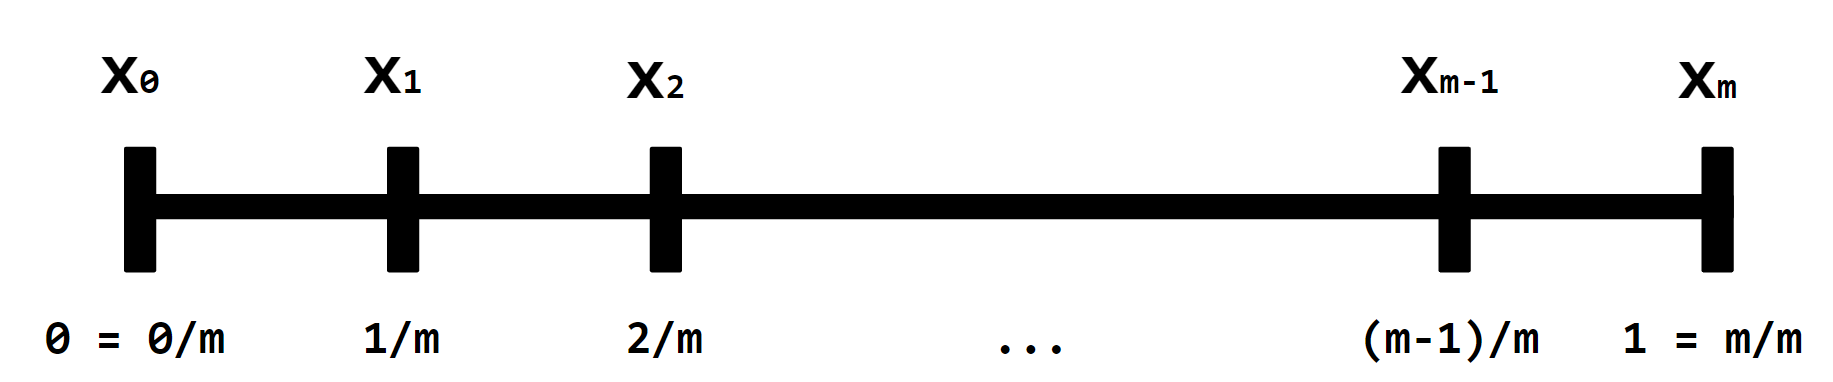
\includegraphics[scale=0.4]{assets/sub_divide.png}
    \end{center}
    
    The subdivision points of the intervals would be $x_i = \frac{i}{m}$ for $i = 0, 1, 2, \hdots, m$. That way, we can find $u$ on those points; that is, we can find \[u\left(x_i = \frac{i}{m}\right).\] 
    With this in mind, the approximation formula from (\ref{1-14:5}) can be rewritten as such:
    \[u'(x_i) \approx \frac{u(x_i + h) - u(x_i)}{h} \approx \frac{u(x_i) - u(x_i - h)}{h} \approx \frac{u(x_i + h) - u(x_i - h)}{2h},\]
    or just 
    \[u'(x_i) \approx \frac{u(x_{i + 1}) - u(x_{i})}{h} \approx \frac{u(x_i) - u(x_{i - 1})}{h} \approx \frac{u(x_{i + 1}) - u(x_{i - 1})}{2h}.\] 
    The approximation used depends on the information you are given.
    \item Now, we can set up a linear system. We want to find $u(x_i)$ for all $i \in [0, m]$. 
    \begin{itemize}
        \item For $i = 0$, it's clear that 
        \[u(x_i) = u(x_0) = u(0) = 0\]
        from the given condition.

        \item For $i = 1$, we can use the approximation 
        \[u'(x_i) \approx \frac{u(x_i) - u(x_{i - 1})}{h}\]
        to get 
        \begin{equation*}
            \begin{aligned}
                &\frac{u(x_1) - u(x_0)}{h} + au(x_1) = f(x_1) \\ 
                    &\implies \frac{u(x_1) - u(0)}{\frac{1}{m}} + au(x_1) = f(x_1) \\ 
                    &\implies mu(x_1) + au(x_1) = f(x_1) \\ 
                    &\implies mu\left(\frac{1}{m}\right) + au\left(\frac{1}{m}\right) = f\left(\frac{1}{m}\right) \\ 
                    &\implies u\left(\frac{1}{m}\right) (m + a) = f\left(\frac{1}{m}\right) \\ 
                    &\implies u\left(\frac{1}{m}\right) = \frac{f\left(\frac{1}{m}\right)}{m + a}
            \end{aligned}
        \end{equation*}

        \item For $i = 2$, we can use the approximation
        \[u'(x_i) \approx \frac{u(x_i) - u(x_{i - 1})}{h}\]
        to get 
        \begin{equation*}
            \begin{aligned}
                &\frac{u(x_2) - u(x_1)}{h} + au(x_2) = f(x_2) \\ 
                    &\implies \frac{u(x_2) - u(x_1)}{\frac{1}{m}} + au(x_2) = f(x_2) \\ 
                    &\implies m\left(u(x_2) - u(x_1)\right) + au(x_2) = f(x_2) \\ 
                    &\implies mu(x_2) - mu(x_1) + au(x_2) = f(x_2) \\ 
                    &\implies u(x_2)(m + a) - mu(x_1) = f(x_2) \\ 
                    &\implies u(x_2)(m + a) = mu(x_1) + f(x_2) \\ 
                    &\implies u(x_2) = \frac{mu(x_1) + f(x_2)}{m + a} \\ 
                    &\implies u\left(\frac{2}{m}\right) = \frac{mu\left(\frac{1}{m}\right) + f\left(\frac{2}{m}\right)}{m + a}.
            \end{aligned}
        \end{equation*}
        Note that we found $u\left(\frac{1}{m}\right)$ in the previous step.

        \item For $i = m$, we have 
        \begin{equation*}
            \begin{aligned}
                &\frac{u(x_m) - u(x_{m - 1})}{h} + au(x_m) = f(x_m) \\ 
                    &\implies \frac{u(1) - u(x_{m - 1})}{\frac{1}{m}} + au(1) = f(1) \\ 
                    &\implies m(u(1) - u(x_{m - 1})) + au(1) = f(1) \\ 
                    &\implies mu(1) - mu(x_{m - 1}) + au(1) = f(1) \\ 
                    &\implies u(1)(m + a) - mu(x_{m - 1}) = f(1) \\ 
                    &\implies u(1)(m + a) = mu(x_{m - 1}) + f(1) \\ 
                    &\implies u(1) = \frac{mu(x_{m - 1}) + f(1)}{m + a} \\ 
                    &\implies u(1) = \frac{mu(\frac{m - 1}{m}) + f(1)}{m + a}.
            \end{aligned}
        \end{equation*}
    \end{itemize}
\end{enumerate}

With this all in mind, we want to be able to generate a linear system of the form 
\begin{equation*}
    \begin{aligned}
        &\begin{cases}
            u\left(\frac{1}{m}\right) = \frac{f\left(\frac{1}{m}\right)}{m + a} \\ 
            u\left(\frac{2}{m}\right) = \frac{mu\left(\frac{1}{m}\right) + f\left(\frac{2}{m}\right)}{m + a} \\ 
            \vdots \\ 
            u(1) = \frac{mu(\frac{m - 1}{m}) + f(1)}{m + a}
        \end{cases} \\ 
        &\implies \begin{cases}
            (m + a) u\left(\frac{1}{m}\right) = f\left(\frac{1}{m}\right) \\ 
            (m + a) u\left(\frac{2}{m}\right) = mu\left(\frac{1}{m}\right) + f\left(\frac{2}{m}\right) \\ 
            \vdots \\ 
            (m + a) u(1) = mu(\frac{m - 1}{m}) + f(1)
        \end{cases} \\ 
        &\implies \begin{cases}
            (m + a) u\left(\frac{1}{m}\right) = f\left(\frac{1}{m}\right) \\ 
            -mu\left(\frac{1}{m}\right) + (m + a) u\left(\frac{2}{m}\right) = f\left(\frac{2}{m}\right) \\ 
            \vdots \\ 
            -mu(\frac{m - 1}{m}) + (m + a) u(1) = f(1)
        \end{cases}.
    \end{aligned}
\end{equation*}
Representing it with matrices, we have 
\begin{equation*}
    \begin{aligned}
        \begin{bmatrix}
            m + a & 0 & 0 & \hdots & 0 \\ 
            -m & m + a & 0 & \hdots & 0 \\ 
            0 & -m & m + a & \hdots & 0 \\ 
            \vdots & \vdots & \vdots & & \vdots \\ 
            0 & 0 & 0 & \hdots & m + a
        \end{bmatrix} \begin{bmatrix}
            u(x_1) \\ u(x_2) \\ u(x_3) \\ \vdots \\ u(x_m)
        \end{bmatrix} = \begin{bmatrix}
            f\left(\frac{1}{m}\right) \\ 
            f\left(\frac{2}{m}\right) \\ 
            f\left(\frac{3}{m}\right) \\ 
            \vdots \\ 
            f\left(\frac{m}{m}\right)
        \end{bmatrix}.
    \end{aligned}
\end{equation*}
\textbf{Remarks:}
\begin{itemize}
    \item Note that if you choose a different approximation, you will get a different left-hand and right-hand side.
    \item A larger $m$ gives a better approximation, but the resulting linear system is larger as well. 
\end{itemize}
Ultimately, the goal here is to solve the linear system $A\x = \b$ to find $u(x_1), u(x_2), \hdots, u(x_m)$. This is the approximation to $u$.

\subsection{Solving Diagonal Systems}
Let's start with the simplest kind of linear system to solve.
\[\begin{bmatrix}
    a_{11} & 0 & 0 & \hdots & 0 \\ 
    0 & a_{22} & 0 & \hdots & 0 \\ 
    0 & 0 & a_{33} & \hdots & 0 \\ 
    \vdots & \vdots & \vdots & & \vdots  \\ 
    0 & 0 & 0 & \hdots & a_{nn}
\end{bmatrix} \begin{bmatrix}
    x_1 \\ x_2 \\ x_3 \\ \vdots \\ x_n
\end{bmatrix} = \begin{bmatrix}
    b_1 \\ b_2 \\ b_3 \\ \vdots \\ b_n
\end{bmatrix}.\]
Writing this as a system of linear equations gives 
\[\begin{cases}
    a_{11}x_1 + 0x_2 + \hdots + 0x_n = b_1 \\ 
    0x_1 + a_{22}x_2 + \hdots + 0x_n = b_2 \\ 
    \vdots \\ 
    0x_1 + 0x_2 + \hdots + a_{nn}x_n = b_n 
\end{cases} \implies \begin{cases}
    a_{11}x_1 = b_1 \\ 
    a_{22}x_2 = b_2 \\ 
    \vdots \\ 
    a_{nn}x_n = b_n 
\end{cases}.\]
The solution is just 
\[x_1 = \frac{b_1}{a_{11}} \qquad x_2 = \frac{b_2}{a_{22}} \qquad \hdots \qquad x_n = \frac{b_n}{a_{nn}}.\]
We can write an algorithm to solve this as well. 
\begin{algorithmic}
    \State $\x \gets \mathbf{0}$
    \For{$i = 1, \hdots, n$}
        \State $x_i \gets \frac{\b_i}{A_{ii}}$
    \EndFor
\end{algorithmic}
From this, it follows that the flop count is just $n$, and its Big-O is $\BigO(n)$. 


\section{Triangular Systems (Section 1.3)}
Generally, it's common practice to reduce general systems down to a triangular form, generally through a process known as Gaussian elimination. They are also easy to solve, and can be solved inexpensively. 

\subsection{Lower and Upper Triangular Matrices}
We say that $L \in \R^{n \times n}$ is a \textbf{lower triangular} matrix if $\ell_{ij} = 0$ whenever $i < j$. Thus, a lower triangular matrix has the form 
\[A = \begin{bmatrix}
    \ell_{11} & 0 & 0 & 0 & 0 & \hdots & 0 \\ 
    \ell_{21} & \ell_{22} & 0 & 0 & 0 & \hdots & 0 \\ 
    \ell_{31} & \ell_{32} & \ell_{33} & 0 & 0 & \hdots & 0 \\ 
    \ell_{41} & \ell_{42} & \ell_{43} & \ell_{44} & 0 & \hdots & 0 \\ 
    \ell_{51} & \ell_{52} & \ell_{53} & \ell_{54} & \ell_{55} & \hdots & 0 \\
    \vdots & \vdots & \vdots & \vdots & \vdots & \ddots & \vdots \\  
    \ell_{n1} & \ell_{n2} & \ell_{n3} & \ell_{n4} & \ell_{n5} & \hdots & \ell_{nn}
\end{bmatrix}.\]
Similarly, we say that $U \in \R^{n \times n}$ is an \textbf{upper triangular} matrix if $u_{ij} = 0$ whenever $i > j$; they have the form 
\[A = \begin{bmatrix}
    u_{11} & u_{12} & u_{13} & u_{14} & u_{15} & \hdots & u_{1n} \\ 
    0 & u_{22} & u_{23} & u_{24} & u_{25} & \hdots & u_{2n} \\ 
    0 & 0 & u_{33} & u_{34} & u_{35} & \hdots & u_{3n} \\ 
    0 & 0 & 0 & u_{44} & u_{45} & \hdots & u_{4n} \\ 
    0 & 0 & 0 & 0 & u_{55} & \hdots & u_{5n} \\
    \vdots & \vdots & \vdots & \vdots & \vdots & \ddots & \vdots \\  
    0 & 0 & 0 & 0 & 0 & \hdots & u_{nn}
\end{bmatrix}.\]
A \textbf{triangular matrix} is one that is either upper or lower triangular.

\begin{mdframed}
    (Example.) Consider the following matrix \[\begin{bmatrix}
        2 & 0 & 0 \\ 
        4 & -1 & 0 \\ 
        -2 & 0 & 3
    \end{bmatrix}.\]
    This is a \textbf{lower triangular matrix}. 
\end{mdframed}
\textbf{Remarks:} 
\begin{itemize}
    \item We can have 0's in the places where there are normally nonzero numbers. This does not violate the definition of a lower- or upper-triangular matrix. 
    \item Because of this, we can say that a diagonal matrix is both a lower- and upper-triangular matrix.
\end{itemize} 

\subsection{Uniqueness of Solution}
When is there a unique system to $L\x = \b$ or $U\x = \b$? 

\begin{mdframed}
    A triangular system (lower or upper) has a unique solution if and only if \emph{all \underline{diagonal} entries} are non-zero.
\end{mdframed}

In fact, as long as the \emph{determinant} of the triangular matrix $A$ is not 0, there will be a unique solution. With triangular matrices, computing the determinant is easy: we just need to multiply all the elements on the \emph{diagonal} together. More technically, as long as 
\[\det(A) = a_{11} \cdot a_{22} \cdot a_{33} \cdot \hdots \cdot a_{nn} \neq 0,\]
then $A\x = \b$ will be a unique solution.

\subsection{Solving Lower Triangular Systems: Forward Substitution}
Suppose we want to solve the following system 
\[\begin{bmatrix}
    \ell_{11} & 0 & 0 & \hdots & 0  \\ 
    \ell_{21} & \ell_{22} & 0 & \hdots & 0  \\ 
    \ell_{31} & \ell_{32} & \ell_{33} & \hdots & 0  \\ 
    \vdots & \vdots & \vdots & \ddots & \vdots \\ 
    \ell_{n1} & \ell_{n2} & \ell_{n3} & \hdots & \ell_{nn}
\end{bmatrix} \begin{bmatrix}
    x_1 \\ x_2 \\ x_3 \\ \vdots \\ x_n
\end{bmatrix} = \begin{bmatrix}
    b_1 \\ b_2 \\ b_3 \\ \vdots \\ b_n
\end{bmatrix}.\]
Notice that \[\ell_{11} x_1 = b_1 \implies x_1 = \frac{b_1}{\ell_{11}}.\]
Also notice that \[\ell_{21} x_1 + \ell_{22}x_2 = b_2 \implies \ell_{22}x_2 = b_2 - \ell_{21}x_1 \implies x_2 = \frac{b_2 - \ell_{21} x_1}{\ell_{22}}.\]
And then notice that \[\ell_{31} x_1 + \ell_{32} x_2 + \ell_{33} x_3 = b_3 \implies \ell_{33}x_3 = b_3 - \ell_{31}x_1 - \ell_{32}x_2 \implies x_3 = \frac{b_3 - \ell_{31}x_1 - \ell_{32}x_2}{\ell_{33}}.\]
Notice how we started off with a simple linear equation, which gave us the answer for $x_1$, and then we can use $x_1$ to find $x_2$ easily in the next equation, and so on. This algorithm is known as \textbf{forward substitution}. For $i = 1, \hdots, n$, it makes use of the formula 
\[\boxed{x_i = \frac{b_i - \ell_{i1} x_1 - \ell_{i2} x_2 - \hdots - \ell_{i,i - 1} x_{i - 1}}{\ell_{ii}} = \frac{b_i - \sum_{j = 1}^{i - 1} \ell_{ij} x_j}{\ell_{ii}}.}\]
Roughly speaking, the algorithm looks like the following:
\begin{algorithmic}
    \For{$i = 1, \hdots, n$}
        \For{$j = 1, \hdots, i - 1$}
            \State $x_i \gets x_i - \ell_{ij} x_j$
        \EndFor

        \If{$g_{ii} = 0$}
            \State Set Error Flag, Exit 
        \EndIf

        \State $x_i \gets x_i / \ell_{ii}$
    \EndFor
\end{algorithmic}

\subsection{Solving Upper Triangular Systems: Backwards Substitution}
Suppose we have an upper triangular matrix $U$, vector $\x$, and $\b$ like so: 
\[U = \begin{bmatrix}
    u_{11} & u_{12} & \hdots & u_{1n}  \\ 
    0 & u_{22} & \hdots & u_{2n} \\ 
    0 & 0 & \hdots & u_{3n} \\
    \vdots & \vdots & \ddots & \vdots \\  
    0 & 0 & 0 & u_{nn}
\end{bmatrix}, \qquad \x = \begin{bmatrix}
    x_1 \\ x_2 \\ x_3 \\ \vdots \\ x_n
\end{bmatrix}, \qquad \b = \begin{bmatrix}
    b_1 \\ b_2 \\ b_3 \\ \vdots \\ b_n
\end{bmatrix}.\]
Suppose we want to solve for $\x$ in $U\x = \b$. First, notice how 
\[\begin{cases}
    u_{nn} x_n = b_n \\ 
    u_{n - 1, n - 1} x_{n - 1} + u_{n - 1, n} x_n = b_{n - 1} \\ 
    u_{n - 2, n - 2} x_{n - 2} + u_{n - 2, n - 1} x_{n - 1} + u_{n - 2, n} x_n = b_{n - 2} \\ 
    \vdots 
\end{cases}.\]
Solving the equations above gives
\[\begin{cases}
    x_n = \frac{b_n}{u_{nn}} \\ 
    x_{n - 1} = \frac{b_{n - 1} - u_{n - 1, n}x_n}{u_{n - 1}} \\ 
    x_{n - 2} = \frac{b_{n - 2} - u_{n - 2, n - 1}x_{n - 1} - u_{n - 2, n}x_n}{u_{n - 2}} \\ 
    \vdots 
\end{cases}\]
Generalizing this, we have 
\[u_{ii}x_i + u_{i, i + 1}x_{i + 1} + \hdots + u_{in}x_n = b_i.\]
Solving for $x_i$ yields
\[\boxed{x_i = \frac{b_i - \left(u_{i, i + 1}x_{i + 1} + \hdots + u_{i, n} x_n\right)}{u_{ii}} = \frac{b_i - \sum_{j = i + 1}^{n} u_{ij}x_j}{u_{ii}}},\]
which is known as \textbf{backwards substitution}.



\section{Gaussian Elimination and the LU Decomposition (Section 1.7)}
We'll now consider the problem of \emph{solving} a system of $n$ linear equations in $n$ unknowns \[A\x = \b\] by Gaussian elimination. Here, we'll assume that $A$ is invertible\footnote{There's a unique solution $\x$, go find it!} and, as usual, $n \times n$. No special properties of $A$ are assumed (e.g., not triangular, not symmetric, not positive definite.).

\begin{mdframed}
    \textbf{Strategy:} We want to transform $A\x = \b$ into an \emph{equivalent system} $U\x = \y$ with $U$ being an upper triangular matrix. Then, we can use back substitution to obtain the solution.
\end{mdframed}

\subsection{Elementary Transformations}
The following transformations can be performed on a system of linear equations, which will not change the solution. Note that we'll assume the use of matrices to represent the problem. 
\begin{enumerate}
    \item Add a multiple of one row to another row.
    \[R_i \mapsto R_i + cR_j,\]
    where $c$ is the multiple. 

    \item Interchange two rows (also known as pivoting). 
    \[R_i \leftrightarrow R_j\]

    \item Multiply a row by a non-zero scalar. 
    \[R_i \mapsto cR_i,\]
    where $c$ is the non-zero scalar.
\end{enumerate}
These transformations will be applied to a system of the form $\begin{bmatrix}
    A & \b
\end{bmatrix}$. 

\subsection{Applying Elementary Operations}
For now, we'll talk about Gaussian Elimination (GE) \underline{without} row interchanges (pivoting). For now, we'll assume that $a_{11} \neq 0$. We want to convert all entries under $a_{11}$ to 0. 

\begin{enumerate}
    \item First, let's get rid of $a_{21}$. We can use the operation \[R_2 \mapsto R_2 - \frac{a_{21}}{a_{11}} R_1\] to do just this: 
    \[\underbrace{\begin{bmatrix}
        a_{11} & a_{12} & a_{13} & \hdots & a_{1n} \\ 
        a_{21} & a_{22} & a_{23} & \hdots & a_{2n} \\ 
        a_{31} & a_{32} & a_{33} & \hdots & a_{3n} \\ 
        \vdots & \vdots & \vdots & \ddots & \vdots \\ 
        a_{n1} & a_{n2} & a_{n3} & \hdots & a_{nn}
    \end{bmatrix}}_{A} \underbrace{\begin{bmatrix}
        b_1 \\ b_2 \\ b_3 \\ \vdots \\ b_n
    \end{bmatrix}}_{\b} \xrightarrow[R_2 \mapsto R_2 - \frac{a_{21}}{a_{11}} R_1]{\text{Type (1) operation.}} \begin{bmatrix}
        a_{11} & a_{12} & a_{13} & \hdots & a_{1n} \\ 
        0      & a_{22}^{(1)} & a_{23}^{(1)} & \hdots & a_{2n}^{(1)} \\ 
        a_{31} & a_{32} & a_{33} & \hdots & a_{3n} \\ 
        \vdots & \vdots & \vdots & \ddots & \vdots \\ 
        a_{n1} & a_{n2} & a_{n3} & \hdots & a_{nn}
    \end{bmatrix} \begin{bmatrix}
        b_1 \\ b_2^{(1)} \\ b_3 \\ \vdots \\ b_n
    \end{bmatrix}.\]
    Note that, while we were able to get rid of $a_{21}$, the other entries in row 2 ($a_{22}$, $a_{23}$, and so on) were updated (hence $a_{22}^{(1)}$, $a_{23}^{(1)}$, and so on). We should also note that $b_2$ was updated, since each row operation affects the \emph{entire} row, which means both the $A$ and the $\b$. 

    \item Next, let's get rid of $a_{31}$. Very similarly to the previous step, we can do
    \[\begin{bmatrix}
        a_{11} & a_{12} & a_{13} & \hdots & a_{1n} \\ 
        0      & a_{22}^{(1)} & a_{23}^{(1)} & \hdots & a_{2n}^{(1)} \\ 
        a_{31} & a_{32} & a_{33} & \hdots & a_{3n} \\ 
        \vdots & \vdots & \vdots & \ddots & \vdots \\ 
        a_{n1} & a_{n2} & a_{n3} & \hdots & a_{nn}
    \end{bmatrix} \begin{bmatrix}
        b_1 \\ b_2^{(1)} \\ b_3 \\ \vdots \\ b_n
    \end{bmatrix} \xrightarrow[R_3 \mapsto R_3 - \frac{a_{31}}{a_{11}}R_1]{\text{Type (1) operation.}} \begin{bmatrix}
        a_{11} & a_{12} & a_{13} & \hdots & a_{1n} \\ 
        0      & a_{22}^{(1)} & a_{23}^{(1)} & \hdots & a_{2n}^{(1)} \\ 
        0      & a_{32}^{(1)} & a_{33}^{(1)} & \hdots & a_{3n}^{(1)} \\ 
        \vdots & \vdots & \vdots & \ddots & \vdots \\ 
        a_{n1} & a_{n2} & a_{n3} & \hdots & a_{nn}
    \end{bmatrix} \begin{bmatrix}
        b_1 \\ b_2^{(1)} \\ b_3^{(1)} \\ \vdots \\ b_n
    \end{bmatrix}\]

    \item Suppose we want to get rid of $a_{i1}$. This is just 
    \[R_i \mapsto R_i - \frac{a_{i1}}{a_{11}}R_1\]
    for $i = 3, \hdots, n$. So, this gives us 
    \[\begin{bmatrix}
        a_{11} & a_{12} & a_{13} & \hdots & a_{1n} \\ 
        0      & a_{22}^{(1)} & a_{23}^{(1)} & \hdots & a_{2n}^{(1)} \\ 
        0      & a_{32}^{(1)} & a_{33}^{(1)} & \hdots & a_{3n}^{(1)} \\ 
        \vdots & \vdots & \vdots & \ddots & \vdots \\ 
        0      & a_{n2}^{(1)} & a_{n3}^{(1)} & \hdots & a_{nn}^{(1)}
    \end{bmatrix} \begin{bmatrix}
        b_1 \\ b_2^{(1)} \\ b_3^{(1)} \\ \vdots \\ b_n^{(1)}
    \end{bmatrix}.\]
\end{enumerate}

Next, we want to get rid of $a_{32}^{(1)}$, $a_{42}^{(1)}$, and so on\footnote{We omit $a_{22}^{(1)}$ because, remember, our goal is to make our system into an upper-triangular system.}. Let's assume that $a_{22}^{(1)} \neq 0$.

\begin{enumerate}
    \item Let's get rid of $a_{32}$. To do this, we'll use the operation
    \[R_3 \mapsto R_3 - \frac{a_{32}^{(1)}}{a_{22}^{(1)}} R_2.\]
    This gives us 
    \[\begin{bmatrix}
        a_{11} & a_{12} & a_{13} & \hdots & a_{1n} \\ 
        0      & a_{22}^{(1)} & a_{23}^{(1)} & \hdots & a_{2n}^{(1)} \\ 
        0      & a_{32}^{(1)} & a_{33}^{(1)} & \hdots & a_{3n}^{(1)} \\ 
        \vdots & \vdots & \vdots & \ddots & \vdots \\ 
        0      & a_{n2}^{(1)} & a_{n3}^{(1)} & \hdots & a_{nn}^{(1)}
    \end{bmatrix} \begin{bmatrix}
        b_1 \\ b_2^{(1)} \\ b_3^{(1)} \\ \vdots \\ b_n^{(1)}
    \end{bmatrix} \xrightarrow[R_3 \mapsto R_3 - \frac{a_{32}^{(1)}}{a_{22}^{(1)}} R_2]{\text{Type (1) operation.}} \begin{bmatrix}
        a_{11} & a_{12} & a_{13} & \hdots & a_{1n} \\ 
        0      & a_{22}^{(1)} & a_{23}^{(1)} & \hdots & a_{2n}^{(1)} \\ 
        0      & 0       & a_{33}^{(2)} & \hdots & a_{3n}^{(2)} \\ 
        \vdots & \vdots & \vdots & \ddots & \vdots \\ 
        0      & a_{n2} & a_{n3} & \hdots & a_{nn}
    \end{bmatrix} \begin{bmatrix}
        b_1 \\ b_2^{(1)} \\ b_3^{(2)} \\ \vdots \\ b_n
    \end{bmatrix}.\]

    \item Likewise, we can repeat this for $a_{i2}$ using the operation 
    \[R_i \mapsto R_i - \frac{a_{i2}^{(1)}}{a_{22}^{(1)}} R_2\]
    for $i = 4, \hdots, n$. This gives us 
    \[\begin{bmatrix}
        a_{11} & a_{12} & a_{13} & \hdots & a_{1n} \\ 
        0      & a_{22}^{(1)} & a_{23}^{(1)} & \hdots & a_{2n}^{(1)} \\ 
        0      & 0       & a_{33}^{(2)} & \hdots & a_{3n}^{(2)} \\ 
        \vdots & \vdots & \vdots & \ddots & \vdots \\ 
        0      & 0       & a_{n3}^{(2)} & \hdots & a_{nn}^{(2)}
    \end{bmatrix} \begin{bmatrix}
        b_1 \\ b_2^{(1)} \\ b_3^{(2)} \\ \vdots \\ b_n^{(2)}
    \end{bmatrix}.\]
\end{enumerate}

We can continue this procedure until we produce an upper-triangular matrix. This upper-triangular matrix will look like 
\[\begin{bmatrix}
    a_{11} & a_{12} & a_{13} & \hdots & a_{1n} \\ 
    0      & a_{22}^{(1)} & a_{23}^{(1)} & \hdots & a_{2n}^{(1)} \\ 
    0      & 0       & a_{33}^{(2)} & \hdots & a_{3n}^{(2)} \\ 
    \vdots & \vdots & \vdots & \ddots & \vdots \\ 
    0      & 0       & 0            & \hdots & a_{nn}^{(n - 1)}
\end{bmatrix} \begin{bmatrix}
    b_1 \\ b_2^{(1)} \\ b_3^{(2)} \\ \vdots \\ b_n^{(n - 1)}
\end{bmatrix}.\]
At the very end, we can use back substitution on the upper-triangular matrix. 

\bigskip 

\textbf{Remark:} We are dividing by $a_{11}$, $a_{22}^{(1)}$, $a_{33}^{(2)}$, and so on for a general matrix. In reality, \emph{some of these entries could be 0}. 

\subsection{LU Decomposition}
\begin{theorem}{LU Decomposition}{}
    Let $A$ be an $n \times n$ matrix whose leading principal submatrices are all nonsingular. Then, $A$ can be decomposed in exactly one way into a product 
    \[A = LU,\]
    such that $L$ is unit lower-triangular and $U$ is upper triangular.
\end{theorem}
In other words, 
\[\begin{bmatrix}
    a_{11} & a_{12} & a_{13} & \hdots & a_{1n} \\ 
    a_{21} & a_{22} & a_{23} & \hdots & a_{2n} \\ 
    a_{31} & a_{32} & a_{33} & \hdots & a_{3n} \\ 
    \vdots & \vdots & \vdots & \ddots & \vdots \\ 
    a_{n1} & a_{n2} & a_{n3} & \hdots & a_{nn}
\end{bmatrix} = \begin{bmatrix}
    1 & 0 & 0 & \hdots & 0 \\ 
    \ell_{21} & 1 & 0 & \hdots & 0 \\ 
    \ell_{31} & \ell_{32} & 1 & \hdots & 0 \\ 
    \vdots & \vdots & \vdots & \ddots & \vdots \\ 
    \ell_{n1} & \ell_{n2} & \ell_{n3} & \hdots & 1
\end{bmatrix} \begin{bmatrix}
    u_{11} & u_{12} & u_{13} & \hdots & u_{1n} \\ 
    0 & u_{22} & u_{23} & \hdots & u_{2n} \\ 
    0 & 0 & u_{33} & \hdots & u_{3n} \\
    \vdots & \vdots & \vdots & \ddots & \vdots \\ 
    0 & 0 & 0 & \hdots & u_{nn}
\end{bmatrix}.\]

\begin{mdframed}
    (Exercise: LU Decomposition.) Let \[A = \begin{bmatrix}
        1 & 3 & 4 \\ 1 & 2 & 6 \\ 3 & 5 & 7
    \end{bmatrix}, \b = \begin{bmatrix}
        1 \\ 1 \\ 1
    \end{bmatrix}.\] Solve $A\x = \b$ for $\x$. 

    \begin{mdframed}
        \begin{equation*}
            \begin{aligned}
                \begin{bmatrix}
                    1 & 3 & 4 \\ 
                    1 & 2 & 6 \\ 
                    3 & 5 & 7
                \end{bmatrix} \begin{bmatrix}
                    1 \\ 1 \\ 1 
                \end{bmatrix} &\xrightarrow[R_2 \mapsto R_2 - R_1]{\text{Operation (1)}} \begin{bmatrix}
                    1 & 3 & 4 \\ 
                    0 & -1 & 2 \\ 
                    3 & 5 & 7
                \end{bmatrix} \begin{bmatrix}
                    1 \\ 0 \\ 1 
                \end{bmatrix} \\ 
                    &\xrightarrow[R_3 \mapsto R_3 - 3R_1]{\text{Operation (1)}} \begin{bmatrix}
                        1 & 3 & 4 \\ 
                        0 & -1 & 2 \\ 
                        0 & -4 & -5
                    \end{bmatrix} \begin{bmatrix}
                        1 \\ 0 \\ -2 
                    \end{bmatrix} \\ 
                    &\xrightarrow[R_3 \mapsto R_3 - 4R_2]{\text{Operation (1)}} \begin{bmatrix}
                        1 & 3 & 4 \\ 
                        0 & -1 & 2 \\ 
                        0 & 0 & -13
                    \end{bmatrix} \begin{bmatrix}
                        1 \\ 0 \\ -2 
                    \end{bmatrix}
            \end{aligned}
        \end{equation*}
        Notice that our matrix is in upper-triangular form. From here, we just need to solve 
        \[\begin{cases}
            -13x_3 = -2 \\ 
            -1x_2 + 2x_3 = 0 \\ 
            x_1 + 3x_2 + 4x_3 = 1
        \end{cases},\]
        which can be done via backwards substitution.

        \bigskip 

        We performed three operations to get to the upper-triangular matrix. Each operation corresponds to a lower-triangular matrix. In particular, if we write out 
        \[\tilde{L_1} \tilde{L_2} \tilde{L_3} A = U,\]
        where each of the $L_i$ represents a lower-triangular matrix and corresponds to an operation, then $\tilde{L_3}$ represents the first operation, $R_2 \mapsto R_2 - R_1$, or $\tilde{L_3} = \begin{bmatrix}
            1 & 0 & 0 \\ 
            -1 & 1 & 0 \\ 
            0 & 0 & 1
        \end{bmatrix}$. Likewise, $\tilde{L_2}$ represents the second operation, $R_3 \mapsto R_3 - 3R_1$, or $\tilde{L_2} = \begin{bmatrix}
            1 & 0 & 0 \\ 
            0 & 1 & 0 \\ 
            -3 & 0 & 1
        \end{bmatrix}$. Finally, $\tilde{L_1}$ represents the third operation, $R_3 \mapsto R_3 - 4R_2$, or $\tilde{L_1} = \begin{bmatrix}
            1 & 0 & 0 \\ 
            0 & 1 & 0 \\ 
            0 & -4 & 1
        \end{bmatrix}$. 
        Notice how the positioning of the numbers corresponds to the entry that we tried to eliminate in $A$. For example, in $L_2$, we put $-3$ in position $L_{21}$ because we eliminated the $3$ from position $A_{21}$ in the second operation. Therefore, 
        \[\begin{bmatrix}
            1 & 0 & 0 \\ 
            0 & 1 & 0 \\ 
            0 & -4 & 1
        \end{bmatrix} \begin{bmatrix}
            1 & 0 & 0 \\ 
            0 & 1 & 0 \\ 
            -3 & 0 & 1
        \end{bmatrix} \begin{bmatrix}
            1 & 0 & 0 \\ 
            -1 & 1 & 0 \\ 
            0 & 0 & 1
        \end{bmatrix} \begin{bmatrix}
            1 & 3 & 4 \\ 
            1 & 2 & 6 \\ 
            3 & 5 & 7
        \end{bmatrix} = \begin{bmatrix}
            1 & 3 & 4 \\ 
            0 & -1 & 2 \\ 
            0 & 0 & -13
        \end{bmatrix}\]

        
        In any case, we know that 
        \[\underbrace{\tilde{L_1} \tilde{L_2} \tilde{L_3}}_{\tilde{L}} A = U.\]
        Then,
        \[\tilde{L}A = U \implies A = \tilde{L}^{-1} U = LU\]
        where 
        \[L = \tilde{L}.\]
    \end{mdframed}
\end{mdframed}

\textbf{Remark:} To see how each operation corresponds to a lower-triangular matrix, consider $R_2 \mapsto R_2 + 5R_1$: 
\[\begin{bmatrix}
    1 & 0 & 0 \\ 
    5 & 1 & 0 \\ 
    0 & 0 & 1 
\end{bmatrix} \begin{bmatrix}
    a_{11} & a_{12} & a_{13} \\ 
    a_{21} & a_{22} & a_{23} \\ 
    a_{31} & a_{32} & a_{33}
\end{bmatrix} = \begin{bmatrix}
    a_{11} & a_{12} & a_{13} \\ 
    5a_{11} + a_{21} & 5a_{12} + a_{22} & 5a_{13} + a_{23} \\ 
    a_{31} & a_{32} & a_{33}
\end{bmatrix}.\]
Likewise, consider $R_3 \mapsto R_3 + 10R_2$:
\[\begin{bmatrix}
    1 & 0 & 0 \\ 
    0 & 1 & 0 \\ 
    0 & 10 & 0 
\end{bmatrix} \begin{bmatrix}
    a_{11} & a_{12} & a_{13} \\ 
    a_{21} & a_{22} & a_{23} \\ 
    a_{31} & a_{32} & a_{33}
\end{bmatrix} = \begin{bmatrix}
    a_{11} & a_{12} & a_{13} \\ 
    a_{21} & a_{22} & a_{23} \\ 
    10a_{21} + a_{31} & 10a_{22} + a_{32} & a_{23} + a_{33}
\end{bmatrix}.\]


\section{Gaussian Elimination with Pivoting (Section 1.8)}
In the previous section, we discussed Gaussian Elimination \emph{without} row interchanges (i.e., pivoting). In this section, we will now permit row interchanges. Consider the following system, 
\[\begin{bmatrix}
    0 & 4 & 1 \\ 
    1 & 3 & 4 \\ 
    2 & 2 & 5
\end{bmatrix} \begin{bmatrix}
    1 \\ 3 \\ 4
\end{bmatrix}.\]
Notice that this matrix has several properties: 
\begin{itemize}
    \item It's invertible ($\det(A) \neq 0$), therefore a unique solution exists. 
    \item However, using Gaussian Elimination \emph{without} row interchanges would fail. 
\end{itemize}
However, we can resolve this by switching two rows, e.g., R1 and R3, to get 
\[\begin{bmatrix}
    2 & 2 & 5 \\ 
    1 & 3 & 4 \\ 
    0 & 4 & 1
\end{bmatrix} \begin{bmatrix}
    4 \\ 3 \\ 1
\end{bmatrix}.\]
When deciding which two rows to switch, the rule is to use the row with the \emph{first} entry containing the \textbf{largest absolute value}\footnote{The reason why we choose the largest absolute value is because dividing by small numbers can cause errors, and these errors can accumulate.}. The idea is that we'll divide by first element in next step for Gaussian elimination.

\subsection{Relation to the Permutation Matrix}
Note taht a permutation matrix $P$ is a matrix which only contains 0's and 1's such that each row and each column has exactly one entry equal to 1. 

\begin{center}
    \begin{tabular}{p{3in}|p{3in}}
        \textbf{Example of Permutation Matrix} & \textbf{\underline{Not} a Permutation Matrix} \\ 
        \hline 
        \[\begin{bmatrix}
            0 & 1 & 0 \\ 
            1 & 0 & 0 \\ 
            0 & 0 & 1 
        \end{bmatrix}\] & \[\begin{bmatrix}
            0 & 1 & 1 \\ 
            1 & 0 & 0 \\ 
            0 & 0 & 1
        \end{bmatrix}\]
        This matrix has two 1's in the first row and last column.
    \end{tabular}
\end{center}
How does the permutation matrix work in relation to row interchanges?

\begin{mdframed}[nobreak=true]
    (Example.) Suppose we multiply a permutation matrix, 
    \[P = \begin{bmatrix}
        0 & 0 & 1 \\ 
        0 & 1 & 0 \\ 
        1 & 0 & 0
    \end{bmatrix},\]
    on the left. 
    \[\begin{bmatrix}
        0 & 0 & 1 \\ 
        0 & 1 & 0 \\ 
        1 & 0 & 0
    \end{bmatrix} \begin{bmatrix}
        0 & 4 & 1 \\ 
        1 & 3 & 4 \\ 
        2 & 2 & 5
    \end{bmatrix} = \begin{bmatrix}
        2 & 2 & 5 \\ 
        1 & 3 & 4 \\ 
        0 & 4 & 1
    \end{bmatrix}.\]
    This corresponds to switching R1 and R3. 
\end{mdframed}

\begin{mdframed}
    (Example.) Suppose we multiply the same permutation matrix as in the previous example on the right. Then, 
    \[\begin{bmatrix}
        0 & 4 & 1 \\ 
        1 & 3 & 4 \\ 
        2 & 2 & 5
    \end{bmatrix} \begin{bmatrix}
        0 & 0 & 1 \\ 
        0 & 1 & 0 \\ 
        1 & 0 & 0
    \end{bmatrix} = \begin{bmatrix}
        1 & 4 & 0 \\ 
        4 & 3 & 1 \\ 
        5 & 2 & 2
    \end{bmatrix}.\]
    Here, this corresponds to switching C1 and C3. 
\end{mdframed}

\subsection{PLU Decomposition}
Gaussian Elimination with pivoting leads to a decomposition of the form $PA = LU$, also known as \emph{PLU decomposition}, where 
\begin{itemize}
    \item $P$ is a permutation matrix,
    \item $L$ is a lower-triangular matrix, and 
    \item $U$ is an upper-triangular matrix. The PLU exists if $A$ is invertible. 
\end{itemize}
\textbf{Remarks:}
\begin{itemize}
    \item The PLU exists if $A$ is invertible. 
    \item In MATLAB, we can run \code{[P, L, U] = lu(A)}, where 
    \[P \cdot A = L \cdot U \implies A = P^T \cdot L \cdot U.\]
\end{itemize}

\subsubsection{Finding PLU Decomposition}
We'll find the PLU decomposition through an example. 

\begin{mdframed}
    (Example.) Suppose we want to find the PLU decomposition of 
    \[A = \begin{bmatrix}
        0 & 4 & 1 \\ 
        1 & 3 & 4 \\ 
        2 & 2 & 5
    \end{bmatrix}.\]

    \begin{itemize}
        \item Step 1: First, let's switch R1 and R3. 
        \[P_1 = \begin{bmatrix}
            0 & 0 & 1 \\ 
            0 & 1 & 0 \\ 
            1 & 0 & 0 
        \end{bmatrix}, \qquad P_1 A = \begin{bmatrix}
            2 & 2 & 5 \\ 
            1 & 3 & 4 \\ 
            0 & 4 & 1
        \end{bmatrix}.\]

        \item Step 2: Next, let's perform the operation $R_2 \mapsto R_2 - \frac{1}{2} R_1$.
        \[L_1 = \begin{bmatrix}
            1 & 0 & 0 \\ 
            -\frac{1}{2} & 1 & 0 \\ 
            0 & 0 & 1
        \end{bmatrix}, \qquad L_1 P_1 A = L_1 \begin{bmatrix}
            2 & 2 & 5 \\ 
            1 & 3 & 4 \\ 
            0 & 4 & 1
        \end{bmatrix} = \begin{bmatrix}
            2 & 2 & 5 \\ 
            0 & 2 & \frac{3}{2} \\ 
            0 & 4 & 1
        \end{bmatrix}.\]

        \item Step 3: Next, notice that \textbf{4} is a pivot (the 2 in the second row is smaller than 4). let's switch $R_2$ and $R_3$.
        \[P_2 = \begin{bmatrix}
            1 & 0 & 0 \\ 
            0 & 0 & 1 \\ 
            0 & 1 & 0
        \end{bmatrix}, \qquad P_2 L_1 P_1 A = \begin{bmatrix}
            2 & 2 & 5 \\ 
            0 & 4 & 1 \\ 
            0 & 2 & \frac{3}{2}
        \end{bmatrix}.\]

        \item Step 4: We can now perform the operation $R_3 \mapsto R_3 - \frac{1}{2}R_2$. 
        \[L_2 = \begin{bmatrix}
            1 & 0 & 0 \\ 
            0 & 1 & 0 \\ 
            0 & -\frac{1}{2} & 1
        \end{bmatrix}, \qquad L_2 P_2 L_1 P_1 A = \begin{bmatrix}
            2 & 2 & 5 \\ 
            0 & 4 & 1 \\ 
            0 & 0 & 1
        \end{bmatrix}.\]
    \end{itemize}
    Here, we find our upper-triangular matrix \[U = L_2 P_2 L_1 P_1 A = \begin{bmatrix}
        2 & 2 & 5 \\ 
        0 & 4 & 1 \\ 
        0 & 0 & 1
    \end{bmatrix}.\] Now that we found the upper-triangular matrix $U$, we need to find the decomposition. We don't know what the $P$ or $L$ matrices are. Notice that, with $L_2 P_2 L_1 P_1$, we can do 
    \[P_2 L_1 = \tilde{L_1} P_2.\] Then, 
    \[L_2 P_2 L_1 P_1 = \underbrace{L_2 \tilde{L_1}}_{\tilde{L}} \overbrace{P_2 P_1}^{P}.\]

    Therefore, if \[P_2 L_1 = \begin{bmatrix}
        1 & 0 & 0 \\ 
        0 & 0 & 1 \\ 
        -\frac{1}{2} & 1 & 0
    \end{bmatrix},\] then
    \begin{equation*}
        \begin{aligned}
            P_2 L_1 &= \tilde{L_1} P_2 \\ 
                &\implies \tilde{L_1} = P_2 L_1 P_2^{-1} \\ 
                &\implies \tilde{L_1} = \begin{bmatrix}
                    1 & 0 & 0 \\ 
                    0 & 0 & 1 \\ 
                    -\frac{1}{2} & 1 & 0
                \end{bmatrix} P_2^{-1} \\ 
                &\implies \tilde{L_1} = \begin{bmatrix}
                    1 & 0 & 0 \\ 
                    0 & 0 & 1 \\ 
                    -\frac{1}{2} & 1 & 0
                \end{bmatrix} \begin{bmatrix}
                    1 & 0 & 0 \\ 
                    0 & 0 & 1 \\ 
                    0 & 1 & 0
                \end{bmatrix} \\ 
                &\implies \tilde{L_1} = \begin{bmatrix}
                    1 & 0 & 0 \\ 
                    0 & 1 & 0 \\ 
                    -\frac{1}{2} & 0 & 1
                \end{bmatrix}.
        \end{aligned}
    \end{equation*}
    Therefore, going back to 
    \[L_2 P_2 L_1 P_1 = \underbrace{L_2 \tilde{L_1}}_{\tilde{L}} \overbrace{P_2 P_1}^{P},\]
    we have 
    \[\tilde{L}PA = U \implies PA = \tilde{L}^{-1} U.\]
    From this, we find 
    \[\tilde{L}^{-1} = \begin{bmatrix}
        1 & 0 & 0 \\ 
        0 & 1 & 0 \\ 
        \frac{1}{2} & 0 & 1
    \end{bmatrix}.\]
    Finally, defining $L = \tilde{L}^{-1}$ gives us 
    \[PA = LU.\]
\end{mdframed}


\section{Positive Definite Systems \& Cholesky Decomposition (Section 1.4)}
In the previous section, we learned about Gaussian Elimination with Pivoting (i.e., $A\x = \b \iff PA = LU$), which can be used to solve \emph{any} system with invertible matrix $A$. However, for some matrix $A$ with special properties, we can use a \emph{better} way to solve it, mainly for computational efficiency.  

\bigskip 

One such class of matrices are \textbf{positive definite} ones. In particular, if $A$ is $n \times n$, real, and satisfies the conditions 
\begin{enumerate}
    \item $A = A^T$ (i.e., symmetric), and 
    \item $\x^T A \x = \begin{bmatrix}
        x_1 & x_2 & \hdots & x_n
    \end{bmatrix} \begin{bmatrix}
        a_{11} & a_{12} & \hdots & a_{1n} \\ 
        a_{21} & a_{22} & \hdots & a_{2n} \\ 
        \vdots & \vdots & \ddots & \vdots \\ 
        a_{n1} & a_{n2} & \hdots & a_{nn}
    \end{bmatrix} \begin{bmatrix}
        x_1 \\ x_2 \\ \vdots \\ x_n
    \end{bmatrix} = \cyclic{x^T, Ax} > 0$ for all nonzero $\x \in \R^n$, 
\end{enumerate}
then $A$ is said to be \textbf{positive definite}. 

\subsection{Properties of Positive Definite Matrix}
There are some useful properties of positive definite matrices. 

\begin{lemma}{}{}
    A positive definite matrix is invertible. 
\end{lemma}

\begin{theorem}{}{}
    Let $M$ be an invertible $n \times n$ matrix. Then, $A = M^T M$ is positive definite.  
\end{theorem}

\begin{theorem}{Cholesky Decomposition Theorem}{}
    Let $A$ be positive definite. Then, there exists an upper-triangular matrix $R$ such that \[A = R^T R.\] This is known as the Cholesky decomposition, and $R$ is called the \textbf{Cholesky factor} of $A$. In addition, this decomposition is unique if we choose $r_{ii} > 0$ for $i = 1, 2, \hdots, n$. 
\end{theorem}

\begin{mdframed}
    (Example: Cholesky Algorithm.) Suppose \[A = \begin{bmatrix}
        a_{11} & a_{12} & a_{13} \\ 
        a_{21} & a_{22} & a_{23} \\ 
        a_{31} & a_{32} & a_{33}
    \end{bmatrix}, \quad R = \begin{bmatrix}
        r_{11} & r_{12} & r_{13} \\ 
        0 & r_{22} & r_{23} \\ 
        0 & 0 & r_{33}
    \end{bmatrix},\]
    so that \[R^T = \begin{bmatrix}
        r_{11} & 0 & 0 \\ 
        r_{21} & r_{22} & 0 \\ 
        r_{31} & r_{32} & r_{33}
    \end{bmatrix}.\] Then, 
    \begin{equation*}
        \begin{aligned}
            \begin{bmatrix}
                a_{11} & a_{12} & a_{13} \\ 
                a_{21} & a_{22} & a_{23} \\ 
                a_{31} & a_{32} & a_{33}
            \end{bmatrix} &= \begin{bmatrix}
                r_{11} & 0 & 0 \\ 
                r_{21} & r_{22} & 0 \\ 
                r_{31} & r_{32} & r_{33}
            \end{bmatrix} \begin{bmatrix}
                r_{11} & r_{12} & r_{13} \\ 
                0 & r_{22} & r_{23} \\ 
                0 & 0 & r_{33}
            \end{bmatrix} \\ 
                &= \begin{bmatrix}
                    r_{11}^2 & r_{11}r_{12} & r_{11}r_{13} \\ 
                    r_{11}r_{12} & r_{12}^2 + r_{22}^2 & r_{12}r_{13} + r_{22} r_{23} \\ 
                    r_{11}r_{13} & r_{13}r_{12} + r_{23}r_{22} & r_{13}^2 + r_{23}^2 + r_{33}^2
                \end{bmatrix}
        \end{aligned}
    \end{equation*}
    One thing to notice is that this matrix is symmetric. So, when finding the values of each element, we only need to find the values of specific elements (one side). We can find the value of each element in $R$. Starting with the first row, we have 
    \begin{itemize}
        \item $r_{11}^2 = a_{11} \implies \boxed{r_{11} = \sqrt{a_{11}}}$.
        \item $r_{11}r_{12} = a_{12} \implies \boxed{r_{12} = \frac{a_{12}}{r_{11}}}$. 
        \item $r_{11}r_{13} = a_{13} \implies \boxed{r_{13} = \frac{a_{13}}{r_{11}}}$.
    \end{itemize}
    For the second row, we have 
    \begin{itemize}
        \item $r_{12}^2 + r_{22}^2 = a_{22} \implies \boxed{r_{22} = \sqrt{a_{22} - r_{12}^2}}$. 
        \item $r_{12}r_{13} + r_{22}r_{23} = a_{23} \implies \boxed{r_{23} = \frac{a_{23} - r_{12}r_{13}}{r_{22}}}$. 
    \end{itemize}
    For the third row, we have 
    \begin{itemize}
        \item $r_{13}^2 + r_{23}^2 + r_{33}^2 = a_{33} \implies \boxed{r_{33} = \sqrt{a_{33} - r_{13}^2 - r_{23}^2}}$. 
    \end{itemize}
\end{mdframed}

The above example is the Cholesky Algorithm for a $3 \times 3$ matrix. For the general case, suppose we have 
\[\underbrace{\begin{bmatrix}
    a_{11} & a_{12} & a_{13} & \hdots & a_{1n} \\ 
    a_{21} & a_{22} & a_{23} & \hdots & a_{2n} \\ 
    a_{31} & a_{32} & a_{33} & \hdots & a_{3n} \\ 
    \vdots & \vdots & \vdots & \ddots & \vdots \\ 
    a_{n1} & a_{n2} & a_{n3} & \hdots & a_{nn}
\end{bmatrix}}_{A} = \underbrace{\begin{bmatrix}
    r_{11} & 0 & 0 & \hdots & 0 \\ 
    r_{21} & r_{12} & 0 & \hdots & 0 \\ 
    r_{31} & r_{23} & r_{33} & \hdots & 0 \\ 
    \vdots & \vdots & \vdots & \ddots & \vdots \\ 
    r_{1n} & r_{2n} & r_{3n} & \hdots & r_{nn}
\end{bmatrix}}_{R^T} \underbrace{\begin{bmatrix} 
    r_{11} & r_{12} & r_{13} & \hdots & r_{1n} \\ 
    0 & r_{22} & r_{23} & \hdots & r_{2n} \\ 
    0 & 0 & r_{33} & \hdots & r_{3n} \\ 
    \vdots & \vdots & \vdots & \ddots & \vdots \\ 
    0 & 0 & 0 & \hdots & r_{nn}
\end{bmatrix}}_{R}.\]
Here, 
\begin{equation}
    a_{ij} = \begin{cases}
        \sum_{k = 1}^{i} r_{ki} r_{kj} & i < j \\ 
        \sum_{k = 1}^{i} r_{ki}^2 & i = j \\ 
        \sum_{k = 1}^{j} r_{ki} r_{kj} & i > j
    \end{cases}
\end{equation}
From this, we're able to solve $r_{ii}$: 
\begin{equation}
    r_{ii} = \sqrt{a_{ii} - \sum_{k = 1}^{i - 1} r_{ki}^2}.
\end{equation}
After solving for $r_{ii}$, we can find $r_{ij}$:
\begin{equation}
    r_{ij} = \frac{\left(a_{ij} - \sum_{k = 1}^{i - 1} r_{ki} r_{kj}\right)}{r_{ii}}.
\end{equation}
for $j = i + 1, \hdots, n$, noting that for $j < i$, $r_{ij} = 0$. 

\bigskip 

In general, Cholesky is doing half of the LU decomposition work: $\BigO(n^3)$. 


\begin{mdframed}
    (Exercise.) Determine whether or not the following matrices have a Cholesky factorization; if they do, compute (by hand) the Cholesky factor $R$.

    \begin{itemize}
        \item $A = \begin{bmatrix}
            1 & -2 & 0 \\ 
            -2 & 13 & 6 \\ 
            0 & 6 & 5
        \end{bmatrix}$

        \begin{mdframed}
            We know that if $R = \begin{bmatrix}
                r_{11} & r_{12} & r_{13} \\ 
                0 & r_{22} & r_{23} \\ 
                0 & 0 & r_{33}
            \end{bmatrix}$ is the Cholesky factor of $A$, then 
            \[r_{11} = \sqrt{1} = 1,\]
            \[r_{12} = \frac{-2}{1} = -2,\]
            \[r_{13} = \frac{0}{1} = 0,\]
            \[r_{22} = \sqrt{13 - (-2)^2} = \sqrt{13 - 4} = \sqrt{9} = 3,\]
            \[r_{23} = \frac{6 - (-2)(0)}{3} = \frac{6}{3} = 2,\]
            \[r_{33} = \sqrt{5 - (0)^2 - (2)^2} = \sqrt{5 - 4} = \sqrt{1} = 1.\]
            Therefore, it follows that the Cholesky factorization is 
            \[R = \begin{bmatrix}
                1 & -2 & 0 \\ 
                0 & 3 & 2 \\ 
                0 & 0 & 1
            \end{bmatrix}\]
            as desired.
        \end{mdframed}

        \item $B = \begin{bmatrix}
            4 & -4 & 0 \\ 
            -4 & 4 & 0 \\ 
            0 & 0 & 5
        \end{bmatrix}.$

        \begin{mdframed}
            We note that 
            \[\det(B) = 4(4 \cdot 5 - 0) - (-4)(-4 \cdot 5 - 0) + 0 = 80 - 80 = 0.\]
            From the contrapositive of the above theorem, because $\det(B) = 0$, it follows that $B$ must not be singular and thus is not positive definite. 
        \end{mdframed}
    \end{itemize}
\end{mdframed}

\begin{mdframed}
    (Exercise.) Consider the following matrix, 
    \[A = \begin{bmatrix}
        1 & 3 & -5 \\ 
        2 & 0 & -4 \\ 
        0 & 1 & 0
    \end{bmatrix}.\] Is it positive definite? 

    \begin{mdframed}
        We can run through the Cholesky Algorithm. 
        \[r_{11} = \sqrt{1} = 1,\]
        \[r_{12} = \frac{3}{1} = 3,\]
        \[r_{13} = \frac{-5}{1} = -5,\]
        \[r_{22} = \sqrt{0 - (1)^2}.\]
        However, we cannot get a real number from $r_{22}$, so $A$ is not positive definite. 
    \end{mdframed}
\end{mdframed}


\section{Vectors and Matrix Norms (Section 2.1)}
In numerical analysis, we want to find approximate solutions to problems (e.g., ODEs). Some things we want to know are 
\begin{itemize}
    \item How good the approximate solution is? 
    \item How close is the approximate solution to the exact solution? 
\end{itemize}
So, \textbf{norms} are a measure of length, or the measure of being close or far apart. 

\subsection{Vector Norms}
The vector norm we're most familiar with is the one in $\R^2$, also known as the \emph{2-norm}. These might look something like
\begin{center}
    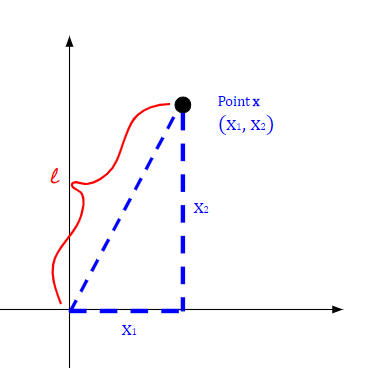
\includegraphics[scale=0.9]{assets/v_norm.png}
\end{center}
For a point \[\x = (x_1, x_2),\] we can define the \emph{2-norm} of a vector to be \[||\x||_2 = \sqrt{x_{1}^{2} + x_{2}^{2}}.\]

\begin{definition}{Vector Norm}{}
    A \textbf{norm} of a vector (i.e., a \textbf{vector norm}) $\x \in \R^n$ is a real number $||\x||$ that is assigned to $\x$. For all $\x, \y \in \R^n$ and all $c \in \R$, the following properties are satisfied: 
    \begin{enumerate}
        \item \underline{Positive Definite Property:} $||\x|| > 0$ for $\x \neq 0$ and $||\0|| = 0$. 
        \item \underline{Absolute Homogeneity:} $||c\x|| = |c| \cdot ||\x||$. 
        \item \underline{Triangle Inequality:} $||\x + \y|| \leq ||\x|| + ||\y||$. 
    \end{enumerate}
\end{definition}
\textbf{Remark:} With regards to the third property, consider \begin{center}
    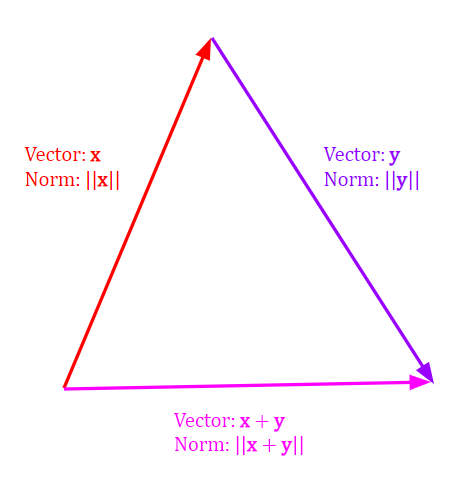
\includegraphics[scale=0.6]{assets/tri_inequality.png}
\end{center}
Note that $||\x + \y|| = ||\x|| + ||\y||$ if $\x$ and $\y$ points at the same direction.

\subsubsection{Common Norms}
There are some common norms that we've seen before. As implied, they all satisfy the properties above. 
\begin{itemize}
    \item For $p \geq 1$, we define 
    \[||\x||_p = \sqrt[p]{|x_1|^p + |x_2|^p + \hdots + |x_n|^p}.\]
    Note that some special cases are 
    \[||\x||_2 = \sqrt{x_1^2 + x_2^2 + \hdots + x_n^2}\]
    and 
    \[||\x||_1 = |x_1| + |x_2| + \hdots + |x_n| = \sum_{i = 1}^{n} |x_i|.\]

    \item The infinite norm is defined to be \[||\x||_{\infty} = \max_{i = 1, 2, \hdots, n} |x_i|.\] It should be noted that \[\lim_{p \mapsto \infty} ||\x||_p = ||\x||_{\infty}.\]
\end{itemize}

\begin{mdframed}
    (Exercise.) Consider the vector, \[\vv = \begin{bmatrix}
        4 \\ 8 \\ 6
    \end{bmatrix}.\]

    \begin{itemize}
        \item Compute $||\vv||_1$.
        \begin{mdframed}
            \[||\vv||_1 = |4| + |8| + |6| = 18.\]
        \end{mdframed}

        \item Compute $||\vv||_2$.
        \begin{mdframed}
            \[||\vv||_2 = \sqrt{4^2 + 8^2 + 6^2} = \sqrt{116}.\]
        \end{mdframed}

        \item Compute $||\vv||_\infty$. 
        \begin{mdframed}
            \[||\vv||_\infty = \max_{i = 1, 2, 3} |v_i| = \max\{|4|, |8|, |6|\} = 8.\]
        \end{mdframed}
    \end{itemize}
\end{mdframed}

\subsection{Matrix Norms}
We now want to consider norms for a matrix $A \in \R^{n \times n}$. There are two ways we can interpret matrix norms.
\begin{enumerate}
    \item Interpret matrix as a vector. For example, suppose we have \[A = \begin{bmatrix}
        -1 & 0 & 5 \\ 8 & 2 & 7 \\ -3 & 1 & 0
    \end{bmatrix}.\] Then, we can ``convert'' this matrix to a vector like so: \[\vv = \begin{bmatrix}
        -1 \\ 0 \\ 5 \\ 8 \\ 2 \\ 7 \\ -3 \\ 1 \\ 0
    \end{bmatrix}.\] Here, $\vv \in \R^9$. Notice how the first column of $A$ is the top three elements in $\vv$, the second column of $A$ is the middle three elements of $\vv$, and the last column of $A$ is the bottom three elements of $\vv$. 

    \item We can also define the matrix as a linear operator. That is, for a function $L: \R^n \mapsto \R^n$, we have \[L(\x) = A\x.\]
\end{enumerate}

\subsubsection{General Definition of Matrix Norms}
\begin{definition}{Matrix Norm}{}
    A \textbf{matrix norm} assigns a real number $||A||$ to a matrix $A$. This should satisfy the following conditions for all $A, B \in \R^{n \times n}$ and $c \in \R$. 
    \begin{enumerate}
        \item $||A|| > 0$ if $A \neq 0$, and $||0|| = 0$. 
        \item $||cA|| = |c| \cdot ||A||$. 
        \item $||A + B|| \leq ||A|| + ||B||$.
        \item Submultiplicity: $||AB|| \leq ||A|| \cdot ||B||$.  
    \end{enumerate}
\end{definition}
\textbf{Remark:} Regarding submultiplicity, for any $\x, \y \in \R^n$, we have \[|\cyclic{x, y}| \leq ||\x||_2 ||y||_2,\] known as the Cauchy Schwarz inequality. 

\subsubsection{Vector Viewpoint}
Going back to the vector viewpoint, let's suppose we have \[A = \begin{bmatrix}
    a_{11} & a_{12} & \hdots & a_{1n} \\ 
    a_{21} & a_{22} & \hdots & a_{2n} \\ 
    \vdots & \vdots & \ddots & \vdots \\ 
    a_{n1} & a_{n2} & \hdots & a_{nn}
\end{bmatrix}.\] Then, 
\[\vv = \begin{bmatrix}
    a_{11} \\ a_{21} \\ \vdots \\ a_{n1} \\ a_{12} \\ a_{22} \\ \vdots \\ a_{n2} \\ \vdots \\ a_{1n} \\ a_{2n} \\ \vdots \\ a_{nn}
\end{bmatrix}.\]

The Frobenius norm of $A$ is defined by 
\[||A||_F = ||\vv||_2 = \left(\sum_{i = 1}^{n} \sum_{j = 1}^{n} |a_{ij}|^2\right)^{\frac{1}{2}}.\]

\subsubsection{Matrix Norm}
Matrix $p$-norms are defined as follows: 
\[||A||_p = \max_{\substack{\x \in \R^n \\ \x \neq \0}} \frac{||A\x||_p}{||\x||_p}.\]
This measures the \emph{maximum stretch} the linear function $L(\x) = A\x$ can do to a vector (normalized by the length of the vector).

\bigskip 

Some of the most important matrix $p$-norms are 
\begin{itemize}
    \item For $p = 1$, \[||A||_1 = \max_{\x \neq \0} \frac{||A\x||_1}{||\x||_1} = \max_{j = 1, 2, \hdots, n} \sum_{i = 1}^{n} |a_{ij}|,\] the maximum $L_1$-norm of each column.
    \item For $p = \infty$, \[||A||_\infty = \max_{\x \neq \0} \frac{||A\x||_\infty}{||\x||_\infty} = \max_{i = 1, 2, \hdots, n} \sum_{j = 1}^{n} |a_{ij}|,\] the maximum $L_1$-norm of each row.
    \item For $p = 2$: \[||A||_2 = \max_{\x \neq \0} \frac{||A\x||_2}{||\x||_2} = \sigma_1,\] the largest\footnote{This is related to SVD, which we will learn later.} singular value of matrix $A$.
\end{itemize}
\textbf{Remark:} Don't confuse $||A||_2$ and $||A||_F$. They are very different! Specifically, 
\[||A||_2 = \max_{\x \neq \0} \frac{||A\x||_2}{||\x||_2}\]
while 
\[||A||_F = ||\vv||_2 = \left(\sum_{i, j} (a_{ij})^2\right)^{\frac{1}{2}}.\]

\begin{mdframed}
    (Exercise.) Consider the following matrix 
    \[A = \begin{bmatrix}
        4 & 8 & 6 \\ 
        8 & 17 & 10 \\ 
        6 & 10 & 29
    \end{bmatrix}.\]

    \begin{itemize}
        \item Compute $||A||_F$.
        \begin{mdframed}
            \[||A||_F = \sqrt{4^2 + 8^2 + 6^2 + 8^2 + 17^2 + 10^2 + 6^2 + 10^2 + 29^2} = \sqrt{1546}.\]
        \end{mdframed}

        \item Compute $||A||_1$.
        \begin{mdframed}
            We consider the sum of the absolute value of the entries in each column. 
            \begin{itemize}
                \item For the first column, we know that 
                \[\sum_{i = 1}^{3} |a_{i1}| = |4| + |8| + |6| = 18.\]
                \item For the second column, 
                \[\sum_{i = 1}^{3} |a_{i2}| = |8| + |17| + |10| = 35.\]
                \item For the third column, 
                \[\sum_{i = 1}^{3} |a_{i3}| = |6| + |10| + |29| = 45.\]
            \end{itemize}
            Therefore, \[||A||_1 = \max\{18, 35, 45\} = 45.\]
        \end{mdframed}

        \item Compute $||A||_\infty$. 
        \begin{mdframed}
            We consider the sum of the absolute value of the entries in each row. 
            \begin{itemize}
                \item For the first row, 
                \[\sum_{j = 1}^{3} |a_{1j}| = |4| + |8| + |6| = 18.\]
                \item For the second row, 
                \[\sum_{j = 1}^{3} |a_{2j}| = |8| + |17| + |10| = 35.\]
                \item For the third row, 
                \[\sum_{j = 1}^{3} |a_{3j}| = |6| + |10| + |29| = 45.\]
            \end{itemize}
            Therefore, \[||A||_\infty = \max\{18, 35, 45\} = 45.\]
        \end{mdframed}
    \end{itemize}
\end{mdframed}

\section{The Discrete Least Squares Problem (Section 3.1)}
Given points $(t_1, y_1), (t_2, y_2), \hdots, (t_n, y_n)$, we want to find an \emph{approximate function} to fit those points; that is, \[p(t_i) = y_i\] for $i = 1, 2, \hdots, n$. For example, suppose we want to find \[p(t) = a_0 + a_1 t\] or \[p(t) = a_0 + a_1 t + a_2 t^2.\] The idea is that we're just trying to find the \emph{line of best fit} (a line with the smallest margin of error). We're not trying to find a line that passes through all the points, just the one of best fit.
\begin{center}
    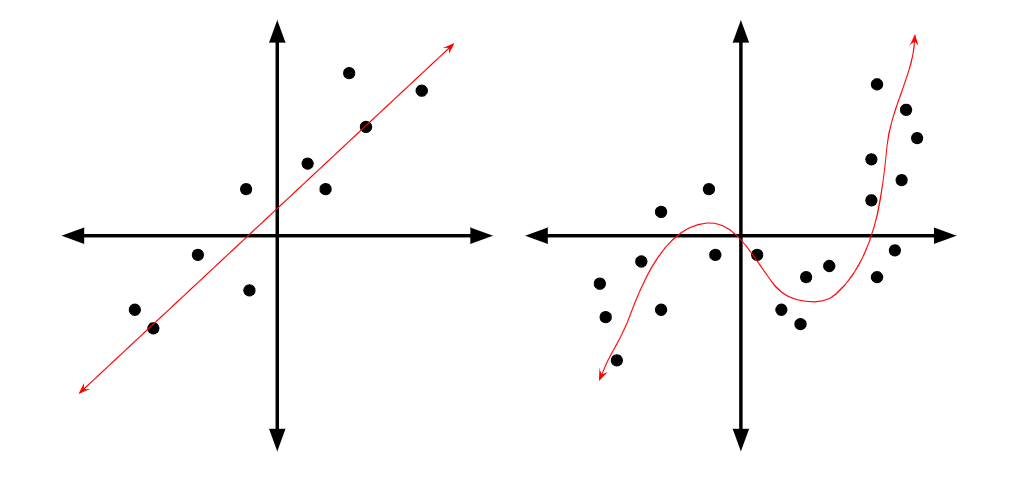
\includegraphics[scale=0.7]{assets/line_best_fit.png}
\end{center}
The error, as mentioned, is defined by $r_i = y_i - p(t_i)$, where $y_i$ is the exact value and $p(t_i)$ is the value of the function (the estimate). Then, the $r_i$'s generate a vector known as the \textbf{residual} vector.

\subsection{Problem Statement}
Our goal is to find a $p(t) = a_0 + a_1 t$ such that $r \in \R^a$ is as small as possible. Hence, it turns into finding $a_0, a_1$ to minimize $||r||_2$. 

\subsubsection{Matrix Notation}
Let's begin by converting 
\[r_i = y_i - p(t_i) = y_i - (a_0 + a_1 t_i) = y_i - a_0 - a_1 t_i \quad i = 1, 2, \hdots, n\]
into matrix notation. This gives us 
\[\underbrace{\begin{bmatrix}
    r_1 \\ r_2 \\ \vdots \\ r_n
\end{bmatrix}}_{\rr \in \R^n} = \begin{bmatrix}
    y_1 - a_0 - a_1 t_1 \\ 
    y_2 - a_0 - a_1 t_2 \\ 
    \vdots \\ 
    y_n - a_0 - a_1 t_n
\end{bmatrix} = \begin{bmatrix}
    y_1 \\ y_2 \\ \vdots \\ y_n
\end{bmatrix} \begin{bmatrix}
    a_0 + a_1 t_1 \\ 
    a_0 + a_1 t_2 \\
    \vdots \\ 
    a_0 + a_1 t_n
\end{bmatrix} = \underbrace{\begin{bmatrix}
    y_1 \\ y_2 \\ \vdots \\ y_n
\end{bmatrix}}_{\y \in \R^n} - \underbrace{\begin{bmatrix}
    1 & t_1 \\ 
    1 & t_2 \\ 
    \vdots & \vdots \\ 
    1 & t_n
\end{bmatrix}}_{A \in \R^{n \times m}} \underbrace{\begin{bmatrix}
    a_0 \\ a_1
\end{bmatrix}}_{\x \in \R^{m}}\]
So, with the above matrix notation, also represented by 
\[\rr = \y - A\x,\]
the goal is to find an $\x \in \R^m$ such that $||\rr||_2$ is minimized. Essentially, 
\[\min_{x \in \R^m} ||\rr||_2 = \min_{x \in \R^m} ||\y - A\x||_2.\] Here, 
\begin{itemize}
    \item $n$ is the number of datapoints, and
    \item $m$ is the number of unknowns from the function. 
\end{itemize} 
\textbf{Remarks:}
\begin{itemize}
    \item $A$ is not squared.
    \item $n > m$.
\end{itemize} 
There will be no solutions\footnote{$A$ has more rows than columns.} to $A\x = \y$. Instead, we want to find $\x$ that minimizes the overall error.

\subsection{Other Basis Functions}
Instead of linear functions $p(t) = a_0 + a_1 t$, we an try other types of functions. For example, consider polynomials, or \[p(t) = a_0 + a_1 t + a_2 t^2 + \hdots + a_k t^k = \sum_{i = 0}^{k} a_i t^i.\] Here, $t^0 = 1$ and we have $(k + 1)$ unknowns. The matrix formulation is given by

\[\underbrace{\begin{bmatrix}
    r_1 \\ r_2 \\ \vdots \\ r_n
\end{bmatrix}}_{r \in \R^n} = \begin{bmatrix}
    y_1 - p(t_1) \\ 
    y_2 - p(t_2) \\ 
    \vdots \\ 
    y_n - p(t_n)
\end{bmatrix} = \begin{bmatrix}
    y_1 \\ y_2 \\ \vdots \\ y_n
\end{bmatrix} - \begin{bmatrix}
    p(t_1) \\ p(t_2) \\ \vdots \\ p(t_n)
\end{bmatrix} = \underbrace{\begin{bmatrix}
    y_1 \\ y_2 \\ \vdots \\ y_n
\end{bmatrix}}_{\y \in \R^n} - \underbrace{\begin{bmatrix}
    1 & t_1 & t_1^2 & \hdots & t_1^k \\ 
    1 & t_2 & t_2^2 & \hdots & t_2^k \\ 
    \vdots & \vdots & \vdots & \ddots & \vdots \\ 
    1 & t_n & t_n^2 & \hdots & t_n^k
\end{bmatrix}}_{A \in \R^{nn \times (k + 1)}} \underbrace{\begin{bmatrix}
    a_0 \\ a_1 \\ \vdots \\ a_k
\end{bmatrix}}_{\x \in \R^{k + 1}}.\]

Here, $\rr = \y - A\x$ is called the \emph{residual}. To solve this, we will use the QR decomposition. 

\subsection{QR Decomposition}
In essence, QR decomposition states that we can decompose a matrix $A$ into two matrices, $Q$ and $R$, such that 
\[A = QR,\]
where $Q$ is orthogonal and $R$ is upper-triangular. 

\subsubsection{A Brief Review}
\begin{definition}{Orthogonal Matrix}{}
    $Q \in \R^{n \times n}$ is called \textbf{orthogonal} if $Q^T = Q^{-1}$, i.e., $Q^T Q = QQ^T = I$. 
\end{definition}

\begin{mdframed}
    (Example.) Consider the rotations in $\R^n$. Note that 
    \[Q = \begin{bmatrix}
        \cos\theta & -\sin\theta \\ 
        \sin\theta & \cos\theta
    \end{bmatrix} \quad Q^T = \begin{bmatrix}
        \cos\theta & \sin\theta \\ 
        -\sin\theta & \cos\theta 
    \end{bmatrix}.\]
    It follows that \[QQ^T = \begin{bmatrix}
        1 & 0 \\ 0 & 1
    \end{bmatrix} = I.\]
\end{mdframed}

\begin{theorem}{}{}
    If $Q \in \R^{n \times n}$ is an orthogonal matrix, then 
    \begin{enumerate}
        \item $\cyclic{Q\x, Q\y} = \cyclic{\x, \y}$. 
        \item $||Q\x||_2 = ||\x||_2$.
    \end{enumerate}    
\end{theorem}
It might be useful to consider this visualization: 
\begin{center}
    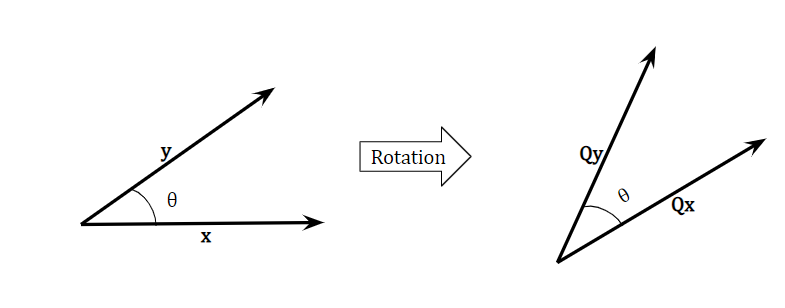
\includegraphics[scale=0.8]{assets/angle_orth.png}
\end{center}

\begin{proof}
    We'll prove each part. 
    \begin{enumerate}
        \item $\cyclic{Q\x, Q\y} = (Q\x)^T Q\y = \x^T Q^T Q \y = \x^T \y = \cyclic{\x, \y}$. 
        \item $||Q\x||_2 = \sqrt{\cyclic{Q\x, Q\y}} = \sqrt{\cyclic{\x, \x}} = ||\x||_2$. 
    \end{enumerate}
    Thus, we're done.
\end{proof}


\section{Solutions to the Discrete Least Squares Problem (Section 3.3)}
In the previous section, we learned how to construct a Least Squares Problem given a set of points. The idea was to find a function such that the residual was minimized. We talked briefly about using QR decomposition and how it could be used to solve this problem. Now, we'll talk more about using QR decomposition. 

\begin{theorem}{Full QR Decomposition}{}
    Let $A \in \R^{n \times m}$ such that $n \geq m$. Then, there exists an orthogonal $Q \in \R^{n \times n}$ and $R \in \R^{n \times m}$ with 
    \[R = \begin{bmatrix}
        r_{11} & r_{12} & \hdots & r_{1m} \\ 
        0 & r_{22} & \hdots & r_{2m} \\
        0 & 0 & \hdots & r_{3m} \\ 
        \vdots & \vdots & \ddots & \vdots \\ 
        0 & 0 & \hdots & r_{nm} \\ 
        0 & 0 & \hdots & 0 \\ 
        0 & 0 & \hdots & 0 \\ 
        0 & 0 & \hdots & 0 \\ 
        \vdots & \vdots & \ddots & 0 \\ 
        0 & 0 & \hdots & 0
    \end{bmatrix} = \begin{bmatrix}
        \hat{R} \\ 0
    \end{bmatrix},\]
    with $\hat{R} \in \R^{m \times m}$ being an upper-triangular matrix and the 0 being the zero-matrix, such that \[A = QR.\]
\end{theorem}
\textbf{Remark:} If $A$ has full rank ($\text{rank}(A) = \min\{n, m\} = m$) and we choose $n_i > 0$, then the reduced QR is unique. 

\subsection{Purpose of QR}
One of the main purposes of the QR decomposition is to solve the Least Squares Problem. Note that methods like LU and PLU decompositions are not useful because the matrix we're working with is a tall matrix ($n \geq m$). 

\bigskip 

Now, that being said, there are two cases to consider. 
\begin{enumerate}
    \item If $A$ is a square matrix and invertible, then it still has a QR decomposition. Note that 
    \begin{equation*}
        \begin{aligned}
            A\x = \y &\implies QR\x = \y \\ 
                &\implies Q^T Q R \x = Q^T \y \\ 
                &\implies R\x = Q^T \y. 
        \end{aligned}
    \end{equation*}

    \item Otherwise, recall that \[\min_{\x \in \R^m} ||\y - A\x||_{2}^{2}\] with $A \in \R^{n \times m}$ and $n \geq m$. Assume that $A$ has a QR decomposition such that \[A = QR,\] we want to compute \[||\y - A\x||_{2}^{2}.\] Notice that
    \begin{equation*}
        \begin{aligned}
            ||\y - A\x||_2^2 &= ||\y - QR\x||_2^2 \\ 
                &= ||I\y - QR\x||_2^2 \\ 
                &= ||QQ^T \y - QR\x||_2^2 \\ 
                &= ||Q(Q^T \y - R\x)||_2^2 \\ 
                &= ||Q^T \y - R\x||_2^2 && Q \text{ is orthogonal, so} ||Q\x||_2^2 = ||\x||_2^2 \\ 
                &= \left|\left| \begin{bmatrix}
                    \hat{c} \\ d
                \end{bmatrix} - \begin{bmatrix}
                    \hat{R} \\ 0
                \end{bmatrix} \x \right|\right|_2^2 \\ 
                &= \left|\left| \begin{bmatrix}
                    \hat{c} - \hat{R}\x \\ 
                    d 
                \end{bmatrix} \right|\right|_2^2 \\ 
                &= ||\hat{c} - \hat{R}\x||_2^2 + ||d||_2^2
        \end{aligned}
    \end{equation*}

    Recall that we rewrote $R$ so that \[R = \begin{bmatrix}
        \hat{R} \\ \0
    \end{bmatrix}.\] We can rewrite $Q^T \y$ so that \[Q^T \y = \begin{bmatrix}
        \hat{c} \\ d
    \end{bmatrix},\] where $\hat{c}$ and $d$ are vectors of length $m$.  
\end{enumerate}
With this in mind, we have 
\[\min_{\x \in \R^m} ||\y - A\x||_2^2 = \min_{\x \in \R^m} ||\hat{c} - \hat{R}\x||_2^2 + ||d||_2^2.\]
Here, $\min_{\x \in \R^m} ||\hat{c} - \hat{R}\x||_2^2$ is the solution to $\hat{R}\x = \hat{c}$, with $\hat{c} = Q^T \y(1 : m)$ and $\hat{R} = R(1:m, 1:m)$ and $A = QR$ is a QR decomposition. Additionally, $\hat{R}\x = \hat{c}$ has a unique solution $\x$, assuming $\text{rank}(A) = m$ and $\hat{c} - \hat{R}\x = \0$. The norm of the residual is $||d||_2$. 


\begin{mdframed}
    (Example.) Suppose we have $\min_{\x \in \R^m} ||\y - A\x||_2^2$ with \[A = \begin{bmatrix}
        -1 & -1 & 1 \\ 
        1 & 3 & 3 \\ 
        -1 & -1 & 5 \\ 
        1 & 3 & 7
    \end{bmatrix}\] and \[\y = \begin{bmatrix}
        1 \\ 0 \\ -1 \\ 2
    \end{bmatrix}\] and want to find $\x$ by using QR. Because we haven't talked about how to do the QR decomposition, we'll give $Q$ and $R$ now: 
    \begin{equation*}
        \begin{aligned}
            \underbrace{\begin{bmatrix}
                -1 & -1 & 1 \\ 
                1 & 3 & 3 \\ 
                -1 & -1 & 5 \\ 
                1 & 3 & 7
            \end{bmatrix}}_{A \in \R^{4 \times 4}} &= \frac{1}{2} \underbrace{\begin{bmatrix}
                -1 & 1 & -1 & 1 \\ 
                1 & 1 & -1 & -1 \\ 
                -1 & 1 & 1 & -1 \\ 
                1 & 1 & 1 & 1
            \end{bmatrix}}_{Q \in \R^{4 \times 4}} \underbrace{\begin{bmatrix}
                2 & 4 & 2 \\ 
                0 & 2 & 8 \\ 
                0 & 0 & 4 \\ 
                0 & 0 & 0
            \end{bmatrix}}_{R \in \R^{4 \times 3}} \\ 
                &= \begin{bmatrix}
                    -\frac{1}{2} & \frac{1}{2} & -\frac{1}{2} & \frac{1}{2} \\ 
                    \frac{1}{2} & \frac{1}{2} & -\frac{1}{2} & -\frac{1}{2} \\ 
                    -\frac{1}{2} & \frac{1}{2} & \frac{1}{2} & -\frac{1}{2} \\ 
                    \frac{1}{2} & \frac{1}{2} & \frac{1}{2} & \frac{1}{2}
                \end{bmatrix} \begin{bmatrix}
                    2 & 4 & 2 \\ 
                    0 & 2 & 8 \\ 
                    0 & 0 & 4 \\ 
                    0 & 0 & 0
                \end{bmatrix}
        \end{aligned}
    \end{equation*}
    Note that\footnote{Recall that $\hat{R} = R(1:m, 1:m)$. In other words, we take the first $m$ rows and columns from $R$.} \[\hat{R} = \begin{bmatrix}
        2 & 4 & 2 \\ 
        0 & 2 & 8 \\ 
        0 & 0 & 4
    \end{bmatrix}.\] Additionally, note that \[Q^T \y = \begin{bmatrix}
        1 \\ 1 \\ 0 \\ 2
    \end{bmatrix}\] so it follows that \[\hat{c} = \begin{bmatrix}
        1 \\ 1 \\ 0
    \end{bmatrix}.\] Finally, $d = \begin{bmatrix}
        2
    \end{bmatrix} = 2$ (note that $d$ is a vector of the remaining entries after $\hat{c}$). Now, we can solve \[\hat{R}\x = \hat{c}.\] In particular,
    \[\begin{bmatrix}
        2 & 4 & 2 \\ 
        0 & 2 & 8 \\ 
        0 & 0 & 4
    \end{bmatrix} \begin{bmatrix}
        x_1 \\ x_2 \\ x_3
    \end{bmatrix} = \begin{bmatrix}
        1 \\ 1 \\ 0
    \end{bmatrix}.\] This gives us \[\x = \begin{bmatrix}
        -\frac{1}{2} \\ \frac{1}{2} \\ 0
    \end{bmatrix}.\]
    The norm of the residual is $||d||_2 = |2| = 2$. 
\end{mdframed}



\section{Projectors \& Reflectors (Section 3.2)}
In this section, we'll talk about projectors and reflectors, something that's important for QR decomposition.

\subsection{Projectors}
\begin{definition}{Projector}{}
    A \textbf{projector} is a matrix $P$ with \[P^2 = P.\] 
\end{definition}

\begin{definition}{Orthoprojector}{}
    If $P$ is a projector and also symmetric (i.e., $P = P^T$), then $P$ is called an \textbf{orthoprojector}.
\end{definition}

\begin{mdframed}
    (Example.) Suppose $\u \in \R^n$ is a unit vector (i.e., $||\u||_2 = 1$). Then, $P = \u \cdot \u^T$ is an orthoprojector. That is, 
    \[P = \begin{bmatrix}
        u_1 \\ u_2 \\ \vdots \\ u_n
    \end{bmatrix} \begin{bmatrix}
        u_1 & u_2 & \hdots & u_n
    \end{bmatrix} = \begin{bmatrix}
        u_1^2 & u_1 u_2 & \hdots & u_1 u_n \\ 
        u_2 u_1 & u_2^2 & \hdots & u_2 u_n \\ 
        \vdots & \vdots & \ddots & \vdots \\ 
        u_n u_1 & u_n u_1 & \hdots & u_n^2 
    \end{bmatrix}.\]
    To see why $P$ here is an orthoprojector, we'll show that it satisfies some properties. 
    \begin{enumerate}
        \item Definition of a projector.
        \[P^2 = P \cdot P = (\u \cdot \u^T) (\u \cdot \u^T) = \u (\underbrace{\u^T \u}_{1}) \u^T = \u \u^T = P.\]

        \item Definition of an orthoprojector.
        \[P^T = (\u \u^T)^T = (\u^T)^T \u^T = \u\u^T = P.\]
    \end{enumerate}
    There are some additional properties to know for this case. 
    \begin{itemize}
        \item $P\u = \u$:
        \[P\u = (\u\u^T)\u = \u(\underbrace{\u^T \u}_{1}) = \u.\]

        \item If $\vv \perp \u$ (i.e., $\cyclic{\vv, \u} = 0$), then $P\vv = \0$. 
        \[P\vv = (\u\u^T)\vv = \u(\underbrace{\u^T\vv}_{0}) = \0.\]
    \end{itemize}
\end{mdframed}
\textbf{Remarks:} 
\begin{itemize}
    \item Note that if $\u \in \R^{n \times 1}$, then $\u^T \in \R^{1 \times n}$ and so $P$ will be an $n \times n$ matrix.
    \item Note that $\u \u^T \neq \u^T \u$. In particular, $\u \u^T$ is an $n \times n$ matrix while $\u^T \u = \cyclic{\u, \u} = ||\u||_{2}^{2}$. 
\end{itemize}

\subsection{Reflectors}
Reflectors are built by \emph{projectors}.

\begin{definition}{Reflector}{}
    For a unit vector $\u \in \R^n$ (i.e., $||\u||_2 = 1$), $Q = I - 2\u \u^T$ is called a (householder) \textbf{reflector}. 
\end{definition}
\textbf{Remarks:} 
\begin{itemize}
    \item We can rewrite the above with $Q = I - 2P$, where $P = \u \u^T$ is a projector. 
    \item If $\u$ doesn't have unit norm, we can normalize it,
    \[\frac{\u}{||\u||_2},\]
    so that $\left|\left| \frac{\u}{||\u||_2} \right|\right|_2 = \frac{1}{||\u||_2} ||\u||_2 = 1$ (note that $||\u||_2$ is a scalar.) In this sense, we can write 
    \[Q = I - 2 \frac{\u}{||\u||_2} \frac{\u^T}{||\u||_2} = I - 2 \frac{\u\u^T}{||\u||_2^2}.\]
\end{itemize}
There are some properties of $Q = I - 2 \u\u^T$ (where $\u$ is a unit vector) to know.
\begin{enumerate}
    \item $Q\u = -\u$. 
    \[Q\u = (I - 2\u\u^T)\u = \u - 2\u\u^T\u = \u - 2\u = -\u.\]

    \item $Q\vv = \vv$ such that $\vv \perp \u$.
    \[Q\vv = (I - 2\u\u^T)\vv = \vv - 2\u\underbrace{\u^T\vv}_{\0} = \vv.\]

    \item $Q^T = Q$. 
    \[Q^T = (I - 2\u\u^T)^T = (I - 2P)^T = I - 2P^T = I - 2P = Q.\]
    Here, note that $I^T = I$. Additionally, note that $P^T = P$.

    \item $\underbrace{Q^T = Q^{-1}}_{\text{Orthogonal}}$ and $Q = Q^{-1}$ and $Q^T Q = Q^2 = I$. 
    \[Q^2 = QQ = (I - 2P)(I - 2P) = I - 2P - 2P + 4P^2 = I - 4P - 4P^2 = I - 4P + 4P = I.\]
\end{enumerate}

\begin{lemma}{}{}
    For any $\x \in \R^n$ and $\y \in \R^n$ such that \[\y = \begin{bmatrix}
        ||\x||_2 & 0 & 0 & \hdots & 0
    \end{bmatrix}^T,\]
    define $\vv = \x - \y$ and $\u = \frac{\vv}{||\vv||_2}$. Then, 
    \[Q = I - 2\u\u^T\] is a reflector satisfying $Q\x = \y$. 
\end{lemma}
\textbf{Remarks:} 
\begin{itemize}
    \item If $\x = \y$, then $Q = I$.
    \item Alternatively, if $\e_1 = \begin{bmatrix}
        1 & 0 & 0 & \hdots & 0
    \end{bmatrix}^T$, then 
    \[\y = ||\x||_2 \e_1.\] It should be noted that $\e_2 = \begin{bmatrix}
        0 & 1 & 0 & \hdots & 0
    \end{bmatrix}$ and $\e_n = \begin{bmatrix}
        0 & 0 & 0 & \hdots & 1
    \end{bmatrix}$. 
\end{itemize} 

\subsection{QR Decomposition (For the 3rd Time)}
We will talk about reduced QR later; for now, we will focus on full QR. The idea is that, with QR, we'll do something like 
\[Q_n \hdots Q_2 Q_1 A \mapsto R.\]
The idea is that, starting from $A$, we can multiply the reflectors multiple times until we end up with $R$, which is an upper-triangular matrix. This is analogous to LU decomposition, where we did 
\[L_n \hdots L_2 L_1 A \mapsto U.\]

Now, for QR decomposition, given $A \in \R^{n \times m}$ (our ``tall'' matrix), we want to find $QR$. We can rewrite $A$ in column form,
\[A = \begin{bmatrix}
    c_1 & c_2 & c_3 & \hdots & c_i & \hdots & c_m
\end{bmatrix},\] 
where $c_i$ is the $i$th column for $i = 1, 2, \hdots, m$. Recall that we want to derive $R$; that is, we want an upper-triangular matrix. So, starting from the first column, we want to make all the entries under $a_{11}$ 0. We can use a reflector mapping $Q_1$ to map the column,
\[c_1 \mapsto ||c_1|| \e_1\]
where $\e_1 \in \R^n$, so that we end up with
\[Q_1 A = \begin{bmatrix}
    ||c_1|| & * & * & \hdots & * \\ 
    0 & * & * & \hdots & * \\ 
    \vdots & \vdots & \vdots & \ddots & \vdots \\ 
    0 & * & * & \hdots & *
\end{bmatrix} = \begin{bmatrix}
    ||c_1|| & * & * & \hdots & * \\ 
    0 & \underline{*} & \underline{*} & \hdots & \underline{*} \\ 
    \vdots & \vdots & \vdots & \ddots & \vdots \\ 
    0 & \underline{*} & \underline{*} & \hdots & \underline{*}
\end{bmatrix}.\]
From the above matrix, we can represent the underlined stars as a new matrix: \[\tilde{A} = \begin{bmatrix}
    \underline{*} & \underline{*} & \hdots & \underline{*} \\ 
    \vdots & \vdots & \ddots & \vdots \\ 
    \underline{*} & \underline{*} & \hdots & \underline{*}
\end{bmatrix} \in \R^{(n - 1) \times (m - 1)}.\]
So, if we have 
\[\tilde{A} = \begin{bmatrix}
    \tilde{c_2} & \tilde{c_3} & \hdots & \tilde{c_m}
\end{bmatrix},\] we want to define a reflector mapping \[\tilde{Q_2}: \tilde{c_2} \mapsto ||\tilde{c_2}|| \tilde{e_1}\] where $\tilde{e_1} \in \R^{n - 1}$. Now, define \[Q_2 = \begin{bmatrix}
    1 & 0 \\ 
    0 & \tilde{Q_2}
\end{bmatrix}\] so that \[Q_2 Q_1 A = \begin{bmatrix}
    ||c_1|| & * & * & \hdots & * \\ 
    0 & ||\tilde{c_2}|| & * & \hdots & * \\ 
    0 & 0 & * & \hdots & * \\
    \vdots & \vdots & \vdots & \ddots & \vdots \\ 
    0 & 0 & * & \hdots & *
\end{bmatrix} = \begin{bmatrix}
    ||c_1|| & * & * & \hdots & * \\ 
    0 & ||\tilde{c_2}|| & * & \hdots & * \\ 
    0 & 0 & \underline{*} & \hdots & \underline{*} \\
    \vdots & \vdots & \vdots & \ddots & \vdots \\ 
    0 & 0 & \underline{*} & \hdots & \underline{*}
\end{bmatrix}.\] From this, we can define \[B = \begin{bmatrix}
    \underline{*} & \hdots & \underline{*} \\ 
    \vdots & \ddots & \vdots \\ 
    \underline{*} & \hdots & \underline{*}
\end{bmatrix}.\] Continuing this process, we should eventually end up with \[Q_m \hdots Q_1 A = \begin{bmatrix}
    ||c_1|| & * & * & \hdots & * \\ 
    0       & ||\tilde{c_2}|| & * & \hdots & * \\ 
    0       & 0               & ||\tilde{c_3}|| & \hdots & * \\ 
    \vdots  & \vdots          & \vdots          & \ddots & * \\ 
    0       & 0               & 0               & \hdots & ||\tilde{c_m}|| \\ 
    \vdots  & \vdots          & \vdots          & \vdots & \vdots \\ 
    0 & 0 & 0 & 0 & 0
\end{bmatrix} = R.\]
Note that $\tilde{Q}A = R \implies A = QR$. Then, the question becomes: how do we define $Q$? We can define $Q$ as\footnote{Recall that $\tilde{Q}$ is orthogonal.} \[Q = \tilde{Q}^{-1} = \tilde{Q}^{T}.\] 
\textbf{Remarks:}
\begin{itemize}
    \item The product of orthogonal matrices is \textbf{orthogonal}.
    \item The inverse of orthogonal matrices is \textbf{orthogonal}.
    \item Note that full QR is not unique.
\end{itemize}
Now, if $A$ has full rank and $r_{ii} > 0$ (the diagonal on the $R$), then the QR decomposition is unique. Note that 
\begin{itemize}
    \item If $A$ has full rank, then $A$ has $m$ linearly independent columns and $\text{rank}(A) = \min\{n, m\} = m$.
\end{itemize}


\section{Reduced QR (Section 3.4)}
Let's begin with an example from a few sections ago. Suppose we have the following \textbf{full QR decomposition}
\begin{equation*}
    \begin{aligned}
        \underbrace{\begin{bmatrix}
            -1 & -1 & 1 \\ 
            1 & 3 & 3 \\ 
            -1 & -1 & 5 \\ 
            1 & 3 & 7
        \end{bmatrix}}_{A \in \R^{4 \times 4}} &= \begin{bmatrix}
            -\frac{1}{2} & \frac{1}{2} & -\frac{1}{2} & \frac{1}{2} \\ 
            \frac{1}{2} & \frac{1}{2} & -\frac{1}{2} & -\frac{1}{2} \\ 
            -\frac{1}{2} & \frac{1}{2} & \frac{1}{2} & -\frac{1}{2} \\ 
            \frac{1}{2} & \frac{1}{2} & \frac{1}{2} & \frac{1}{2}
        \end{bmatrix} \begin{bmatrix}
            2 & 4 & 2 \\ 
            0 & 2 & 8 \\ 
            0 & 0 & 4 \\ 
            0 & 0 & 0
        \end{bmatrix} \\ 
            &= \frac{1}{2} \underbrace{\begin{bmatrix}
                -1 & 1 & -1 & 1 \\ 
                1 & 1 & -1 & -1 \\ 
                -1 & 1 & 1 & -1 \\ 
                1 & 1 & 1 & 1
            \end{bmatrix}}_{Q \in \R^{4 \times 4}} \underbrace{\begin{bmatrix}
                2 & 4 & 2 \\ 
                0 & 2 & 8 \\ 
                0 & 0 & 4 \\ 
                0 & 0 & 0
            \end{bmatrix}}_{R \in \R^{4 \times 3}}.
    \end{aligned}
\end{equation*}
Here, $Q$ is orthogonal and $R$ is a tall matrix. Let's look at $R$. Notice how the last row of $R$ are just 0's. In particular, the last column of the matrix $Q$ and the last row of $R$ yields 0's everywhere; it's not helpful. So, what if we throw away the last row of $R$ and corresponding columns of $Q$? This brings us to the topic of \textbf{reduced QR}. In particular,
\[\underbrace{\begin{bmatrix}
    -1 & -1 & 1 \\ 
    1 & 3 & 3 \\ 
    -1 & -1 & 5 \\ 
    1 & 3 & 7
\end{bmatrix}}_{A \in \R^{4 \times 4}} = \frac{1}{2} \underbrace{\begin{bmatrix}
    -1 & 1 & -1 \\ 
    1 & 1 & -1 \\ 
    -1 & 1 & 1 \\ 
    1 & 1 & 1
\end{bmatrix}}_{\hat{Q} \in \R^{4 \times 3}} \underbrace{\begin{bmatrix}
    2 & 4 & 2 \\ 
    0 & 2 & 8 \\ 
    0 & 0 & 4
\end{bmatrix}}_{\hat{R} \in \R^{3 \times 3}}.\]
\textbf{Remark:} $\hat{Q}$ is not a square matrix anymore; it's a tall matrix. The concept of orthogonal matrices does not make sense here anymore. Instead, note that $\hat{Q}$ is an \textbf{isometry}; 
\[\underbrace{\hat{Q}^T}_{3 \times 4} \underbrace{\hat{Q}}_{4 \times 3} = \underbrace{I}_{3 \times 3}.\]
(Compare this to orthogonal, where we have $Q^T Q = QQ^T = I$.)

\begin{theorem}{Reduced QR}{}
    Suppose $A \in \R^{n \times m}$ such that $n \geq m$. Then, there exists a $\hat{Q} \in \R^{n \times m}$ isometry and $\hat{R} \in \R^{m \times m}$ upper-triangular such that \[A = \hat{Q}\hat{R}.\]
\end{theorem}
\textbf{Remark:} The reduced QR decomposition is unique if $\text{rank}(A) = m$ and we choose $r_{ii} > 0$ (entry on diagonal of $\hat{R}$). 


\subsection{Orthonormal Set}
Before we talk about how to obtain the reduced QR decomposition, we first introduce orthonormal sets. 
\begin{definition}{Orthonormal Set}{}
    We say that\footnote{Note that $q_i$ is a \emph{vector}.}
    \[\{q_1, q_2, \hdots, q_m\}\]
    is called \textbf{orthonormal} if $\cyclic{q_i, q_j} = 0$ whenever $i \neq j$ and $\cyclic{q_i, q_i} = 1$.
\end{definition}
\textbf{Remark:} If $Q$ is orthogonal (isometry), then the columns are orthonormal. For example, if the set $\{e_1, e_2\}$ is orthonormal, then this might visually look like 
\begin{center}
    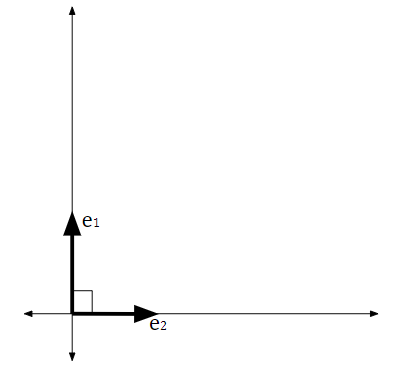
\includegraphics[scale=0.7]{assets/orthonormal.png}
\end{center}

\subsection{Gram-Schmidt}
With the idea of orthonormal sets in mind, the idea is to use the \textbf{Gram-Schmidt} algorithm to make the columns of $A$ into an orthonormal set $\{q_1, q_2, \hdots, q_m\}$. This represents $\hat{Q}$. 

\bigskip 

Notationally, assuming $A$ has full rank (i.e., linearly independent), we can say that \[\{a_1, a_2, \hdots, a_m\}\] represents the columns of $A$. 


\subsubsection{Classical Algorithm}
Given $A$, we want to find $\hat{Q}$ and $\hat{R}$ such that $A = \hat{Q}\hat{R}$. As mentioned above, we can write $A$ as a set of linearly independent columns, 
\[\begin{bmatrix}
    a_1, a_2, \hdots, a_m
\end{bmatrix}.\]
We can also write $\hat{Q}$ in the same way:
\[\begin{bmatrix}
    q_1, q_2, \hdots, q_m
\end{bmatrix}.\]
We can write $\hat{R}$ like so: 
\[\begin{bmatrix}
    r_{11} & r_{12} & \hdots & r_{1m} \\ 
    0 & r_{22} & \hdots & r_{2m} \\ 
    \vdots & \vdots & \ddots & \vdots \\ 
    0 & 0 & \hdots & r_{mm}
\end{bmatrix}.\]
Combining this, we end up with 
\[\begin{bmatrix}
    a_1, a_2, \hdots, a_m
\end{bmatrix} = \begin{bmatrix}
    q_1, q_2, \hdots, q_m
\end{bmatrix} \begin{bmatrix}
    r_{11} & r_{12} & \hdots & r_{1m} \\ 
    0 & r_{22} & \hdots & r_{2m} \\ 
    \vdots & \vdots & \ddots & \vdots \\ 
    0 & 0 & \hdots & r_{mm}
\end{bmatrix}.\]
Then, we note that 
\[a_1 = q_1 r_{11} \implies q_1 = \frac{a_1}{r_{11}} \implies r_{11} = ||a_1||_2.\]
\[a_2 = q_1 r_{12} + q_2 r_{22}.\]
\[a_3 = q_1 r_{13} + q_2 r_{23} + q_3 r_{33}.\]
Eventually, we'll end up with 
\[a_m = q_1 r_{1m} + q_2 r_{2m} + \hdots + q_m r_{mm}.\]
So, this is the basic idea: processing each column one at a time. Writing this out as steps, we have: 
\begin{enumerate}
    \item $r_{11} = ||a_1||_2$, $q_1 = \frac{a_1}{r_{11}} = \frac{a_1}{||a_1||_2}$. It follows that \[||q_1||_2 = 1.\]
    \item $a_2 = r_{12}q_1 + r_{22}q_2$. Then, we can multiply $q_1$ on both sides: 
    \begin{equation*}
        \begin{aligned}
            \cyclic{a_2, q_1} &= \cyclic{r_{12}q_1 + r_{22}q_2, q_1} \\ 
                &= r_{12}\underbrace{\cyclic{q_1, q_1}}_{1} + r_{22} \underbrace{\cyclic{q_2, q_1}}_{0} \\ 
                &= r_{12}.
        \end{aligned}
    \end{equation*}
    Note that we got the 0 and 1 from the properties of orthonormal sets. In any case, it follows that \[q_2 = \frac{a_2 - r_{12}q_1}{r_{22}}.\]
    Setting $r_{22} = ||a_2 - r_{12}q_1||_2$, it follows that $||q_2||_2 = 1$. 

    \item We start from $a_3$ and determine $q_3$ and $r_{13}$, $r_{23}$, and $r_{33}$. 
\end{enumerate}
Notice that we essentially keep going like this. Let's try to generalize this. The formula for $\hat{R}$ is given by 
\[\hat{R} = (r_{ji})\]
for $j < i$. Then, \[\hat{Q} = \begin{bmatrix}
    q_1 & q_2 & \hdots & q_m
\end{bmatrix}\] and we can get $A = \hat{Q} \hat{R}$. Remember that 
\[r_{12} = \cyclic{a_2, q_1}.\] Note that the 1 in $r$ index corresponds to the 1 in $q_1$ and the 2 in the $r$ index corresponds to the 2 in $a_2$. We also know that 
\[r_{22} = ||a_2 - r_{12}q_1||_2\] and 
\[q_2 = \frac{a_2 - r_{12}q_1}{r_{22}}.\]
Analogously, notice that 
\[r_{13} = \cyclic{a_3, q_1}\] and \[r_{23} = \cyclic{a_3, q_2}.\] We also know that \[a_{33} = ||a_3 - r_{13}q_1 - r_{23}q_2||_2\] and \[q_3 = \frac{a_3 - \sum_{j = 1}^{2} r_{j3} q_j}{r_{33}}.\] 
\underline{So, to conclude, we can generalize the formula:}
\[r_{ii} = \left|\left| a_{i} - \sum_{j = 1}^{i - 1} r_{ji} q_j \right|\right|_2.\]
\[r_{ji} = \cyclic{a_i, q_j} \qquad j < i.\]
\[q_i = \frac{a_i - \sum_{j = 1}^{i - 1} r_{ji} q_j}{r_{ii}}.\]
To reiterate the whole process, given $A$, we want to find $\hat{Q}$ and $\hat{R}$ such that 
\begin{equation}{\label{2-6:1}}
    A = \hat{Q}\hat{R}.
\end{equation} Note that we can rewrite ({\ref{2-6:1}}) in the form 
\[\begin{bmatrix}
    a_1 & a_2 & \hdots & a_m
\end{bmatrix} = \begin{bmatrix}
    q_1 & q_2 & \hdots & q_m
\end{bmatrix} \begin{bmatrix}
    r_{11} & r_{12} & \hdots & r_{1m} \\ 
    0      & r_{22} & \hdots & r_{2m} \\ 
    \vdots & \vdots & \ddots & \vdots \\ 
    0      & 0      & 0      & r_{mm} 
\end{bmatrix}.\] 
The formula to finding these entries are 
\[a_m = q_1 r_{1m} + q_2 r_{2m} + \hdots + q_m r_{mm}.\]
\[r_{ji} = \begin{cases}
    \cyclic{a_{i}, q_{j}} & j < i \\ 
    \left|\left| a_i - \sum_{k = 1}^{i - 1} r_{ki} q_k \right|\right|_2 & j = i \\ 
    0 & j > i
\end{cases}.\]
\[q_{i} = \frac{a_i - \sum_{j = 1}^{i - 1} r_{ji} q_j}{r_{ii}}.\]
$a_i$ is a vector and $r_{ij}$ is a scalar. 

\subsubsection{Worked Example}
\begin{mdframed}
    (Example.) Suppose we have \[A = \begin{bmatrix}
        -1 & -1 & 1 \\ 
        1 & 3 & 3 \\ 
        -1 & -1 & 5 \\ 
        1 & 3 & 7
    \end{bmatrix}.\]
    We can define 
    \[\vec{a_1} = \begin{bmatrix}
        -1 \\ 1 \\ -1 \\ 1
    \end{bmatrix} \quad \vec{a_2} = \begin{bmatrix}
        -1 \\ 3 \\ -1 \\ 3
    \end{bmatrix} \quad \vec{a_3} = \begin{bmatrix}
        1 \\ 3 \\ 5 \\ 7
    \end{bmatrix}.\]
    In other words, our goal is to get something like 
    \[A = \begin{bmatrix}
        a_1 & a_2 & a_3
    \end{bmatrix} = \begin{bmatrix}
        q_1 & q_2 & q_3
    \end{bmatrix} \begin{bmatrix}
        r_{11} & r_{12} & r_{13} \\ 
        0 & r_{22} & r_{23} \\ 
        0 & 0 & r_{33}
    \end{bmatrix}.\]
    Then, we can find the elements of $\hat{Q}$ and $\hat{R}$. 
    \begin{mdframed}
        \[a_1 = q_1 r_{11} \implies q_1 = \frac{a_1}{r_{11}}.\]
        Since $q_1$ is a unit vector (remember that the $q_i$'s are in an orthonormal set), it follows that $||q_1||_2 = 1$. Then, 
        \[r_{11} = ||a_{1}||_2 = \sqrt{(-1)^2 + 1^2 + (-1)^2 + 1^2} = 2.\]
        Notice that 
        \[q_1 = \frac{a_1}{2} = \frac{1}{2} \begin{bmatrix}
            -1 \\ 1 \\ -1 \\ 1 
        \end{bmatrix} = \begin{bmatrix}
            -\frac{1}{2} \\ \frac{1}{2} \\ -\frac{1}{2} \\ \frac{1}{2}
        \end{bmatrix}.\]
        \[a_2 = q_1 r_{12} + q_2 r_{22}.\]
        Because $q_1$ and $q_2$ are orthonormal, we know that $\cyclic{q_2, q_2} = 1$ and $\cyclic{q_1, q_2} = 0$. So, \[\cyclic{a_2, q_1} = \cyclic{q_1 r_{12} + q_2 r_{22}, q_1} = r_{12} \underbrace{\cyclic{q_1, q_1}}_{1} + r_{22} \underbrace{\cyclic{q_2, q_1}}_{0} = r_{12}\]
        Then, 
        \begin{equation*}
            \begin{aligned}
                r_{12} &= \cyclic{a_{2}, q_{1}}= \begin{bmatrix}
                        -1 & 3 & -1 & 3
                    \end{bmatrix} \begin{bmatrix}
                        -\frac{1}{2} \\ \frac{1}{2} \\ -\frac{1}{2} \\ \frac{1}{2}
                    \end{bmatrix} \\ 
                    &= (-1) \left(-\frac{1}{2}\right) + (3) \left(\frac{1}{2}\right) + (-1)\left(-\frac{1}{2}\right) + (3)\left(\frac{1}{2}\right) \\ 
                    &= 4.
            \end{aligned}
        \end{equation*}
        Now, we need to find 
        \[q_2 = \frac{a_2 - \sum_{j = 1}^{1} r_{ji}q_j}{r_{22}}.\]
    \end{mdframed}

    \begin{mdframed}
        \begin{itemize}
            \item Note that 
            \begin{equation*}
                \begin{aligned}
                    r_{22} &= \left|\left| a_2 - \sum_{k = 1}^{1} r_{k2} q_k \right|\right|_2 = \left|\left| a_2 - r_{12} q_1 \right|\right|_2 \\ 
                        &= \left|\left| \begin{bmatrix}
                            -1 \\ 3 \\ -1 \\ 3
                        \end{bmatrix} - 4 \begin{bmatrix}
                            -\frac{1}{2} \\ \frac{1}{2} \\ -\frac{1}{2} \\ \frac{1}{2}
                        \end{bmatrix} \right|\right|_2 = \left|\left| \begin{bmatrix}
                            -1 \\ 3 \\ -1 \\ 3
                        \end{bmatrix} - \begin{bmatrix}
                            -2 \\ 2 \\ -2 \\ 2
                        \end{bmatrix} \right|\right|_2 \\ 
                        &= \left|\left| \begin{bmatrix}
                            1 \\ 1 \\ 1 \\ 1
                        \end{bmatrix} \right|\right|_2 = \sqrt{1^2 + 1^2 + 1^2 + 1^2} = \sqrt{4} = 2.
                \end{aligned}
            \end{equation*}
            \item From this, it follows that 
            \[q_2 = \frac{a_2 - r_{12} q_1}{r_{22}} = \frac{1}{r_{22}}(a_2 - r_{12} q_1) = \frac{1}{2}\left(\begin{bmatrix}
                -1 \\ 3 \\ -1 \\ 3
            \end{bmatrix} - 4 \begin{bmatrix}
                -\frac{1}{2} \\ \frac{1}{2} \\ -\frac{1}{2} \\ \frac{1}{2}
            \end{bmatrix}\right) = \frac{1}{2}\begin{bmatrix}
                1 \\ 1 \\ 1 \\ 1
            \end{bmatrix} = \begin{bmatrix}
                \frac{1}{2} \\ \frac{1}{2} \\ \frac{1}{2} \\ \frac{1}{2}
            \end{bmatrix}.\]
        \end{itemize}

        \[a_3 = r_{13} q_1 + r_{23}q_2 + r_{33}q_3.\]
        At this point, we know that 
        \[q_1 = \begin{bmatrix}
            -\frac{1}{2} \\ \frac{1}{2} \\ -\frac{1}{2} \\ \frac{1}{2}
        \end{bmatrix} \quad q_2 = \begin{bmatrix}
            \frac{1}{2} \\ \frac{1}{2} \\ \frac{1}{2} \\ \frac{1}{2}
        \end{bmatrix} \quad a_3 = \begin{bmatrix}
            1 \\ 3 \\ 5 \\ 7
        \end{bmatrix}.\]
        Additionally, $\cyclic{q_1, q_3} = \cyclic{q_2, q_3} = 0$ while $\cyclic{q_3, q_3} = 1$. From there, we have
        \[r_{13} = \cyclic{a_3, q_1} = \begin{bmatrix}
            1 & 3 & 5 & 7
        \end{bmatrix} \begin{bmatrix}
            -\frac{1}{2} \\ \frac{1}{2} \\ -\frac{1}{2} \\ \frac{1}{2}
        \end{bmatrix} = 1\left(-\frac{1}{2}\right) + 3\left(\frac{1}{2}\right) + 5\left(-\frac{1}{2}\right) + 7\left(\frac{1}{2}\right) = 2\]
        and 
        \[r_{23} = \cyclic{a_3, q_2} = \begin{bmatrix}
            1 & 3 & 5 & 7
        \end{bmatrix} \begin{bmatrix}
            \frac{1}{2} \\ \frac{1}{2} \\ \frac{1}{2} \\ \frac{1}{2}
        \end{bmatrix} = 8\]
    \end{mdframed}

    \begin{mdframed}
        and 
        \begin{equation*}
            \begin{aligned}
                r_{33} &= \left|\left| a_3 - \sum_{k = 1}^{2} r_{k3} q_k \right|\right|_2 \\ 
                    &= \left|\left| a_3 - (r_{13} q_1 + r_{23} q_2) \right|\right|_2 \\ 
                    &= \left|\left| \begin{bmatrix}
                        1 \\ 3 \\ 5 \\ 7
                    \end{bmatrix} - \left(2 \begin{bmatrix}
                        -\frac{1}{2} \\ \frac{1}{2} \\ -\frac{1}{2} \\ \frac{1}{2}
                    \end{bmatrix} + 8 \begin{bmatrix}
                        \frac{1}{2} \\ \frac{1}{2} \\ \frac{1}{2} \\ \frac{1}{2}
                    \end{bmatrix}\right) \right|\right|_2 \\ 
                    &= \left|\left| \begin{bmatrix}
                        -2 \\ -2 \\ 2 \\ 2
                    \end{bmatrix} \right|\right|_2 \\ 
                    &= \sqrt{(-2)^2 + (-2)^2 + 2^2 + 2^2} \\ 
                    &= \sqrt{4 + 4 + 4 + 4} \\ 
                    &= 4.
            \end{aligned}
        \end{equation*}
        Finally,
        \begin{equation*}
            \begin{aligned}
                q_3 &= \frac{a_3 - \sum_{j = 1}^{2} r_{j3}q_j}{r_{33}} = \frac{a_3 - (r_{13}q_1 + r_{23}q_2)}{r_{33}} = \frac{1}{r_{33}} (a_3 - (r_{13}q_1 + r_{23}q_2)) \\ 
                    &= \frac{1}{4} \begin{bmatrix}
                        -2 \\ -2 \\ 2 \\ 2
                    \end{bmatrix} = \begin{bmatrix}
                        -\frac{1}{2} \\ -\frac{1}{2} \\ \frac{1}{2} \\ \frac{1}{2}
                    \end{bmatrix}.
            \end{aligned}
        \end{equation*}
    \end{mdframed}

    Notice that we're now done with the algorithm. In particular, we have 
    \[q_1 = \begin{bmatrix}
        -\frac{1}{2} \\ \frac{1}{2} \\ -\frac{1}{2} \\ \frac{1}{2}
    \end{bmatrix} \quad q_2 = \begin{bmatrix}
        \frac{1}{2} \\ \frac{1}{2} \\ \frac{1}{2} \\ \frac{1}{2}
    \end{bmatrix} \quad q_3 = \begin{bmatrix}
        -\frac{1}{2} \\ -\frac{1}{2} \\ \frac{1}{2} \\ \frac{1}{2}
    \end{bmatrix},\]
    and 
    \[r_{11} = 2 \quad r_{12} = 4 \quad r_{13} = 2 \quad r_{22} = 2 \quad r_{23} = 8 \quad r_{33} = 4.\]
    This gives us the decomposition of 
    \[\underbrace{\begin{bmatrix}
        -1 & -1 & 1 \\ 
        1 & 3 & 3 \\ 
        -1 & -1 & 5 \\ 
        1 & 3 & 7
    \end{bmatrix}}_{A} = \underbrace{\begin{bmatrix}
        -\frac{1}{2} & \frac{1}{2} & -\frac{1}{2} \\ 
        \frac{1}{2} & \frac{1}{2} & -\frac{1}{2} \\ 
        -\frac{1}{2} & \frac{1}{2} & \frac{1}{2} \\ 
        \frac{1}{2} & \frac{1}{2} & \frac{1}{2}
    \end{bmatrix}}_{\hat{Q}} \underbrace{\begin{bmatrix}
        2 & 4 & 2 \\ 
        0 & 2 & 8 \\ 
        0 & 0 & 4
    \end{bmatrix}}_{\hat{R}}.\]
\end{mdframed}

\subsubsection{Summary}
This is effectively how the \textbf{classical Gram-Schmidt} algorithm works. Notice how we went through each $\vec{a_i}$ entry (column by column) and found all the desired values of $\vec{q_i}$ and $r_{ij}$. 

\bigskip 

Sadly, the classical Gram-Schmidt is \textbf{unstable}\footnote{A very small change of some entry in $A$ can yield a significant difference in the resulting $QR$ decomposition.}. For this reason, we'll introduce a \emph{modified} Gram-Schmidt algorithm, which is \textbf{stable}. One notable difference is that 
\begin{itemize}
    \item The classical algorithm builds $R$ one \emph{column} at a time. 
    \item The modified algorithm builds $R$ one \emph{row} at a time.
\end{itemize}
\begin{center}
    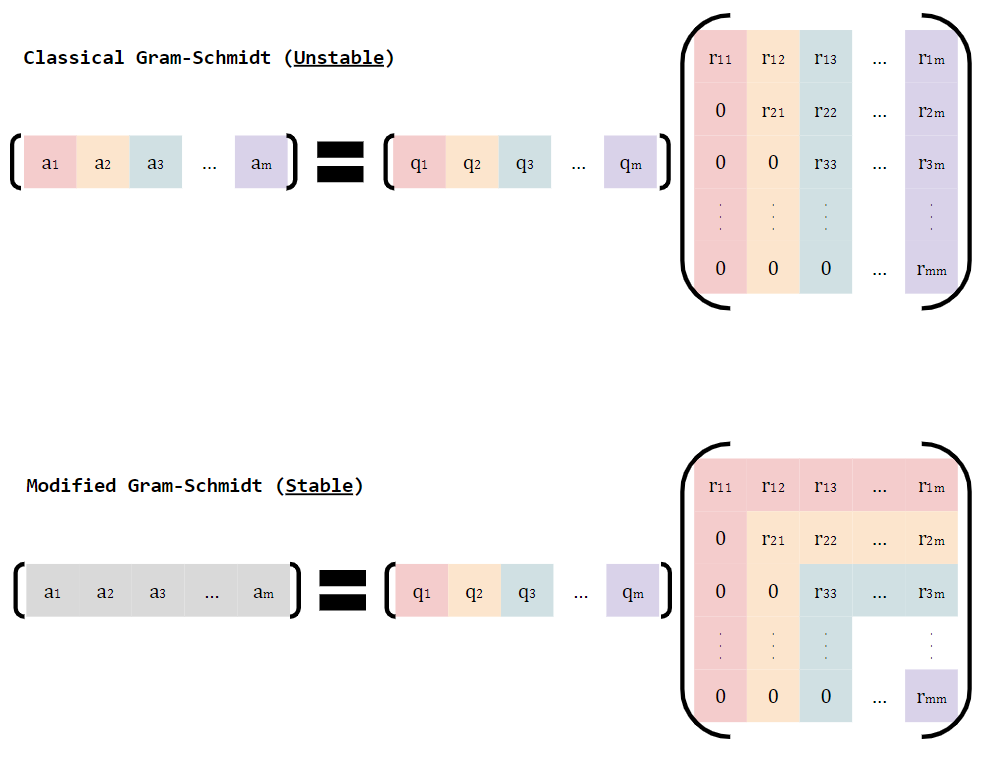
\includegraphics[scale=0.75]{assets/gram.png}
\end{center}

\subsubsection{MATLAB Code}
\begin{mdframed}
    \begin{verbatim}
function [Q,R]=classicalGS(A)         % classical Gram-Schmidt

n = size(A,2);                        % number of columns; this formulation
                                      % does not need the number of rows
for i=1:n                             
Q(:,i) = A(:,i);                      % initialization
   
    for j=1:(i-1)
        R(j,i)=(A(:,i))'*Q(:,j);      % computing R(j,i) by going down the column
        Q(:,i)=Q(:,i)-R(j,i)*Q(:,j);  % updating Q(:,j)
    end
   
    R(i,i) = norm(Q(:,i));            % computing R(i,i) 
    Q(:,i)=Q(:,i)/R(i,i);             % making Q(:,i) a unit vector
end
    \end{verbatim}
\end{mdframed}


\subsection{Modified Gram-Schmidt}
As mentioned earlier, the modified Gram-Schmidt is a stable algorithm that builds $R$ one row at a time. 

\subsubsection{MATLAB Code}
\begin{mdframed}
    \begin{verbatim}
function [Q,R]=modifiedGS(A)          % modified Gram-Schmidt

n = size(A,2);                        % number of columns; this formulation
                                      % does not need the number of rows
for i=1:n                             
    Q(:,i) = A(:,i);                  % initialization
end

for i=1:n
    R(i,i) = norm(Q(:,i));            % computing R(i,i) 
    Q(:,i)=Q(:,i)/R(i,i);             % making Q(:,i) a unit vector

    for j=(i+1):n
        R(i,j)=(Q(:,i))'*Q(:,j);      % computing R(i,j) by going right on ith row
        Q(:,j)=Q(:,j)-R(i,j)*Q(:,i);  % updating Q(:,j)
    end

end
    \end{verbatim}
\end{mdframed}

\subsubsection{Worked Example}
We'll base our algorithm on the MATLAB code above. 
\begin{mdframed}
    (Example.) We'll solve the same problem as in the previous example, \emph{except} we'll use the modified algorithm instead. To reiterate, suppose we have \[A = \begin{bmatrix}
        -1 & -1 & 1 \\ 
        1 & 3 & 3 \\ 
        -1 & -1 & 5 \\ 
        1 & 3 & 7
    \end{bmatrix}.\]
    We can define 
    \[\vec{a_1} = \begin{bmatrix}
        -1 \\ 1 \\ -1 \\ 1
    \end{bmatrix} \quad \vec{a_2} = \begin{bmatrix}
        -1 \\ 3 \\ -1 \\ 3
    \end{bmatrix} \quad \vec{a_3} = \begin{bmatrix}
        1 \\ 3 \\ 5 \\ 7
    \end{bmatrix}.\]
    In other words, our goal is to get something like 
    \[A = \begin{bmatrix}
        a_1 & a_2 & a_3
    \end{bmatrix} = \begin{bmatrix}
        q_1 & q_2 & q_3
    \end{bmatrix} \begin{bmatrix}
        r_{11} & r_{12} & r_{13} \\ 
        0 & r_{22} & r_{23} \\ 
        0 & 0 & r_{33}
    \end{bmatrix}.\]
    \textbf{Keep this in mind}, since we'll be assuming this. Then, we can find the elements of $\hat{Q}$ and $\hat{R}$. We'll run through the algorithm described in code above. 
    \begin{enumerate}
        \item First, we define $q_1 = a_1$, $q_2 = a_2$, and $q_3 = a_3$. 
        
        \item Next, for we want to find $r_{11}$, $r_{12}$, $r_{13}$ and then determine $q_1$. We can also update $q_2$ and $q_3$. 
        
        \begin{itemize}
            \item (Outer Loop: $i = 1$.) Note that 
            \[r_{11} = ||q_1||_2 = ||a_1||_2 = \sqrt{(-1)^2 + 1^2 + (-1)^2 + 1^2} = 2.\]
            Here, $r_{11} = ||q_1||_2$ comes from the algorithm (since we \emph{initially} set $q_1 = a_1$.)
            \[q_1 = \frac{q_1}{r_{11}} = \frac{q_1}{||a_1||_2} = \begin{bmatrix}
                -1/2 \\ 1/2 \\ -1/2 \\ 1/2
            \end{bmatrix}.\]
            Here, we've updated the value of $q_1$. 
    
            \item In the \emph{inner loop}, we do the following for $j = 2$ to $3$:
            \begin{itemize}
                \item (Inner Loop: $j = 2$.) Next, note that 
                \[r_{12} = \cyclic{q_1, q_2} = q_1^T q_2 = q_1^T a_2 = \left(-\frac{1}{2}\right)(-1) + \frac{1}{2}(3) + \left(-\frac{1}{2}\right)(-1) + \frac{1}{2}(3) = 4.\]
                From there, it follows that 
                \[q_2 = q_2 - r_{12}q_1 = \begin{bmatrix}
                    -1 \\ 3 \\ -1 \\ 3
                \end{bmatrix} - 4 \begin{bmatrix}
                    -1/2 \\ 1/2 \\ -1/2 \\ 1/2
                \end{bmatrix} = \begin{bmatrix}
                    1 \\ 1 \\ 1 \\ 1
                \end{bmatrix}.\]
        
                \item (Inner Loop: $j = 3$.) Next, we have 
                \[r_{13} = \cyclic{q_1, q_3} = q_1^T q_3 = q_1^T a_3 = \left(-\frac{1}{2}\right)(1) + \frac{1}{2}(3) + \left(-\frac{1}{2}\right)(5) + \frac{1}{2}7 = 2.\]
                From there, it follows that 
                \[q_3 = q_3 - r_{13}q_1 = \begin{bmatrix}
                    1\\3\\5\\7
                \end{bmatrix} - 2\begin{bmatrix}
                    -1/2 \\ 1/2 \\ -1/2 \\ 1/2
                \end{bmatrix} = \begin{bmatrix}
                    2 \\ 2 \\ 6 \\ 6
                \end{bmatrix}.\]
            \end{itemize}
        \end{itemize}
        
        \item After running through the first iteration of the outer loop discussed in the algorithm, we have 
        \[q_2 = \begin{bmatrix}
            1\\1\\1\\1
        \end{bmatrix} \quad q_3 = \begin{bmatrix}
            2\\2\\6\\6
        \end{bmatrix}.\] 
        Now, we want to find $r_{22}$, $r_{23}$, and determine $q_2$. We also update $q_3$. 
        \begin{itemize}
            \item (Outer Loop: $i = 2$.) We have 
            \[r_{22} = ||q_2||_2 = \sqrt{1^2 + 1^2 + 1^2 + 1^2} = 2.\]
            So, updating $q_2$ gives us 
            \[q_2 = \frac{q_2}{r_{22}} = \begin{bmatrix}
                1/2 \\ 1/2 \\ 1/2 \\ 1/2
            \end{bmatrix}.\] 

            \item In the \emph{inner loop}, we do the following for $j = 3$ to $3$:
            \begin{itemize}
                \item (Inner Loop: $j = 3$.) We have 
                \[r_{23} = \cyclic{q_2, q_3} = q_2^T = q_3 = \frac{1}{2}(2) + \frac{1}{2}(2) + \frac{1}{2}(6) + \frac{1}{2}(6) = 8.\]
                From there, 
                \[q_3 = q_3 - r_{23}q_2 = \begin{bmatrix}
                    2\\2\\6\\6
                \end{bmatrix} - 8\begin{bmatrix}
                    1/2 \\ 1/2 \\ 1/2 \\ 1/2
                \end{bmatrix} = \begin{bmatrix}
                    -2 \\ -2 \\ 2 \\ 2
                \end{bmatrix}.\]
            \end{itemize}
        \end{itemize}

        \item After running through the second iteration of the outer loop discussed in the algorithm, we have 
        \[q_3 = \begin{bmatrix}
            -2 \\ -2 \\ 2 \\ 2
        \end{bmatrix}.\]
        Now, we can find $r_{33}$ and determine the value of $q_3$. 
        \begin{itemize}
            \item (Outer Loop: $i = 3$.) We have 
            \[r_{33} = ||q_3||_2 = \sqrt{(-2)^2 + (-2)^2 + 2^2 + 2^2} = 4.\]
            So, 
            \[q_3 = \frac{q_3}{r_{33}} = \begin{bmatrix}
                -1/2 \\ -1/2 \\ 1/2 \\ 1/2
            \end{bmatrix}.\]

            \item Notice that the inner loop is not executed since $j = 4$ is greater than $3$.
        \end{itemize}
    \end{enumerate}
\end{mdframed}


\section{Condition Numbers \& Perturbation (Section 2.2, 2.3)}
We are now interested in the \emph{sensitivity} of $A\x = \b$ with respect to perturbations (i.e., error). In other words, does noise in $A$ or $\b$ strongly affect the solution $\x$? Here, we'll deal with two types of perturbations: in $\b$, and in $A$. Eventually, we'll talk about the case when there's noise in both. 

\subsection{Motivating Example}
To see what we mean, consider the following two examples.
\begin{mdframed}
    (Example.) Consider the system 
    \[\underbrace{\begin{bmatrix}
        1 & 1 \\ 0 & 1 
    \end{bmatrix}}_A \underbrace{\begin{bmatrix}
        x_1 \\ x_2
    \end{bmatrix}}_{\x} = \underbrace{\begin{bmatrix}
        2 \\ 0
    \end{bmatrix}}_{\b}.\]

    \begin{enumerate}
        \item Solve for $\x$. 
        \begin{mdframed}
            Note that \[\x = \begin{bmatrix}
                2 \\ 0
            \end{bmatrix}\] by backwards substitution.
        \end{mdframed}

        \item Suppose we introduce a very small error to the entries of $\b$ such that $\hat{\b} = \begin{bmatrix}
            2 \\ 0.001
        \end{bmatrix}.$ Our system now becomes \[\underbrace{\begin{bmatrix}
            1 & 1 \\ 0 & 1 
        \end{bmatrix}}_A \underbrace{\begin{bmatrix}
            \hat{x_1} \\ \hat{x_2}
        \end{bmatrix}}_{\hat{\x}} = \underbrace{\begin{bmatrix}
            2 \\ 0.001
        \end{bmatrix}}_{\hat{\b}}.\] Solve for $\hat{\x}$. In other words, what happens to $\x$ if we perturb $\b$?  

        \begin{mdframed}
            Here, we have \[\hat{\x} = \begin{bmatrix}
                1.999 \\ 0.001
            \end{bmatrix}.\]
            Here, $\hat{\x}$ is known as a perturbed solution. Notice how the difference between the solution and the perturbed solution is very small, to the point that both $\x$ and $\hat{x}$ are \emph{similar}.
        \end{mdframed}

        \item Compute the error in $\b$ and in $\x$.
        \begin{mdframed}
            The error in $\b$ can be found by using the $L_2$-norm. So, for $\b$, we have 
            \[||\b - \hat{\b}||_2 = \left|\left| \begin{bmatrix}
                2 \\ 0
            \end{bmatrix} - \begin{bmatrix}
                2 \\ 0.001
            \end{bmatrix} \right|\right|_2 = \left|\left| \begin{bmatrix}
                0 \\ -0.001
            \end{bmatrix} \right|\right|_2 = 0.001\]
            Likewise, for $\x$, we have 
            \[||\x - \hat{\x}||_2 = \left|\left| \begin{bmatrix}
                2 \\ 0
            \end{bmatrix} - \begin{bmatrix}
                1.999 \\ 0.001
            \end{bmatrix} \right|\right|_2 = \left|\left| \begin{bmatrix}
                0.001 \\ -0.001
            \end{bmatrix} \right|\right|_2 = \sqrt{2} \cdot 0.001 \approx 0.0014.\]
        \end{mdframed}
    \end{enumerate}
\end{mdframed}


\begin{mdframed}[nobreak=true]
    (Example.) Consider a similar system 
    \[\underbrace{\begin{bmatrix}
        1 & 1 \\ 0 & 0.001 
    \end{bmatrix}}_A \underbrace{\begin{bmatrix}
        x_1 \\ x_2
    \end{bmatrix}}_{\x} = \underbrace{\begin{bmatrix}
        2 \\ 0
    \end{bmatrix}}_{\b}.\]

    \begin{enumerate}
        \item Solve for $\x$. 
        \begin{mdframed}
            We have 
            \[\x = \begin{bmatrix}
                2 \\ 0
            \end{bmatrix},\] which we found by backwards substitution. 
        \end{mdframed}

        \item Suppose we introduce a very small error to the entries of $\b$ such that $\hat{\b} = \begin{bmatrix}
            2 \\ 0.001
        \end{bmatrix}.$ Our system now becomes \[\underbrace{\begin{bmatrix}
            1 & 1 \\ 0 & 0.001 
        \end{bmatrix}}_A \underbrace{\begin{bmatrix}
            \hat{x_1} \\ \hat{x_2}
        \end{bmatrix}}_{\hat{\x}} = \underbrace{\begin{bmatrix}
            2 \\ 0.001
        \end{bmatrix}}_{\hat{\b}}.\] Solve for $\hat{\x}$.

        \begin{mdframed}
            Here, we have \[\hat{x} = \begin{bmatrix}
                1 \\ 1
            \end{bmatrix}.\]
            One important thing to notice is that the perturbed solution is \emph{quite different} from the actual solution. So, unlike the previous example, $\x$ and $\hat{x}$ are \emph{different}. 
        \end{mdframed}

        \item Compute the error in $\b$ and in $\x$.
        \begin{mdframed}
            The error in $\b$ is the same as in the previous example; therefore,  
            \[||\b - \hat{\b}||_2 = 0.001\]
            But, for $\x$, notice how 
            \[||\x - \hat{\x}||_2 = \left|\left| \begin{bmatrix}
                2 \\ 0
            \end{bmatrix} - \begin{bmatrix}
                1 \\ 1
            \end{bmatrix} \right|\right|_2 = \left|\left| \begin{bmatrix}
                1 \\ -1
            \end{bmatrix} \right|\right|_2 = \sqrt{2} \approx 1.41.\]
            In particular, $0.001$ is $10^3$ larger than 1.41. So, in this linear system, when we perturb $\b$ a little, we can cause a \emph{large} error. 
        \end{mdframed}
    \end{enumerate}
\end{mdframed}

\textbf{Remark:} From this, it follows that the error in $\x$ depends on the matrix $A$ as well. 


\subsection{Condition Number}
How do we measure the dependence on the matrix $A$? This is related to the \textbf{condition number}, known as \code{cond(A)} in MATLAB. The condition number is a simple but useful measure of the sensitivity of the linear system $A\x = \b$. Although we haven't defined the condition number yet, consider the following examples, which showcase the difference in condition number: 
\begin{itemize}
    \item $\cond\left(\begin{bmatrix}
        1 & 1 \\ 0 & 1
    \end{bmatrix}\right) \approx 2.1618$, which is a small condition number. 
    
    \item $\cond\left(\begin{bmatrix}
        1 & 1 \\ 0 & 0.001
    \end{bmatrix}\right) \approx 2 \cdot 10^3$, which is a large condition number, and the error is amplified by this large condition number. 
\end{itemize}

\subsection{Perturbation of \texorpdfstring{$\b$}{b}}
Now, we want to solve $A\x = \b$, where $A$ is invertible. Instead of $\b$, we only have access to \[\hat{\b} = \b + \delta\b,\] where $\delta\b$ is the (very small) error, known as the perturbation in $\b$. Then, we can consider the linear system \[A\hat{\x} = \hat{\b}.\] If $\hat{\b}$ is close to $\hat{\b}$, is it true that $\hat{\x}$ is close to $\hat{\x}$ as well? \textbf{This depends} on the condition number of $A$. In particular, we'll later see that \begin{equation}{\label{2-13:1}}
    \boxed{\frac{||\x - \hat{\x}||}{||\x||} \leq \kappa(A) \frac{||\b - \hat{\b}||}{||\b||}}.
\end{equation} Here, 
\begin{itemize}
    \item $\frac{||\x - \hat{\x}||}{||\x||}$ is the \emph{relative error} of $\x$, 
    \item $\frac{||\b - \hat{\b}||}{||\b||}$ is the \emph{relative error} of $\b$. 
    \item $\kappa(A)$ is the condition number of the invertible matrix $A$.
\end{itemize}
The relative error of $\x$ is bounded by the condition number of matrix $A$ multiplifed by the relative error of $\b$. 

\bigskip 

What is $\kappa(A)$? We can define it like so:  
\[\kappa(A) = ||A|| \cdot ||A^{-1}||,\] where $||\cdot||$ can be any vector norm. We will use the notation 
\begin{itemize}
    \item $\kappa_p$ for the $p$-norm; that is, \[\kappa_{p}(A) = ||A||_p \cdot ||A^{-1}||_p.\]
    \item $\kappa_\infty$ for the $\infty$-norm; that is, \[\kappa_\infty(A) = ||A||_\infty \cdot ||A^{-1}||_\infty.\]
\end{itemize}

With this in mind, let's prove the inequality in (\ref{2-13:1}).
\begin{proof}
    We can break this down into two steps. 
    \begin{itemize}
        \item Let $\hat{\b} = \b + \delta\b$ (the perturbed $\b$) and $\hat{\x} = \x + \delta\x$ (the perturbed $\x$). So, 
        \begin{equation*}
            \begin{aligned}
                A\hat{\x} = \hat{\b} &\implies A(\x + \delta\x) = \b + \delta\b \\ 
                    &\implies A\x + A\delta\x = \b + \delta\b \\ 
                    &\implies A\delta\x = \delta\b && \text{Recall that } A\x = \b \\ 
                    &\implies \delta\x = A^{-1}\delta\b && A \text{ is invertible} \\ 
                    &\implies ||\delta\x|| = ||A^{-1} \delta\b||.
            \end{aligned}
        \end{equation*}
        Recall that $||A|| = \max_{\x \neq \0} \frac{||A\x||}{||\x||}$ is the matrix norm induced by the vector norm. Additionally, note that $||A^{-1}|| = \max_{\x \neq \0} \frac{||A^{-1}\x||}{||\x||}$. Then,
        \[||A^{-1}|| = \max_{\x \neq \0} \frac{||A^{-1}\x||}{||\x||} \geq \frac{||A^{-1}\delta\b||}{||\delta\b||} \implies ||A^{-1}|| \cdot ||\delta\b|| \geq ||A^{-1}\delta\b||.\]
        So, 
        \[||\delta\x|| = ||A^{-1} \delta\b|| \leq ||A^{-1}|| \cdot ||\delta\b|| \implies ||\delta\x|| \leq ||A^{-1}|| \cdot ||\delta\b||.\]

        \item Recall that $\b = A\x$. So, 
        \[\b = A\x \implies ||\b|| = ||A\x|| \leq ||A|| \cdot ||\x||.\]
        Then, we can divide both sides by $||\b|| \cdot ||\x||$ to get 
        \[\frac{1}{||\x||} \leq ||A||\frac{1}{||\b||}.\]
    \end{itemize}
    With all this, we can combine the inequalities
    \[||\delta\x|| \leq ||A^{-1}|| \cdot ||\delta\b||\]
    \[\frac{1}{||\x||} \leq ||A||\frac{1}{||\b||}\]
    to get 
    \[\underbrace{\frac{||\delta\x||}{||\x||}}_{\substack{\text{Relative error} \\ \text{in } \x}} \leq \underbrace{||A^{-1}|| \cdot ||A||}_{\substack{\kappa(A) \\ \text{Condition number.}}} \cdot \underbrace{\frac{||\delta\b||}{||\b||}}_{\substack{\text{Relative error} \\ \text{in } \b}}.\]
   This simplifies to $\frac{||\delta\x||}{||\x||} \leq \kappa(A)\frac{||\delta\b||}{||\b||}$, as desired.  
\end{proof}
\textbf{Remarks:}
\begin{itemize}
    \item The matrix norm is the induced matrix norm, e.g., if the vector norm is 2-norm, then the matrix norm is 2-norm. That is, 
    \[||A||_p = \max_{\x \neq \0} \frac{||A\x||_p}{||\x||_p}\]
    \[||A||_\infty = \max_{\x \neq \0} \frac{||A\x||_\infty}{||\x||_\infty}\]
    This means that we can use whatever vector norm we want for (\ref{2-13:1}) as long as all vectors use the same norm. Additionally, the induced matrix norm for $A$ should be the same as the one used for the vector norm. \textbf{The norms must be consistent in the inequality.}
    \item When interpreting $\kappa(A)$, 
    \begin{itemize}
        \item If $\kappa(A)$ is small (close to 1), then $A$ is called ``well-conditioned.''
        \item If $\kappa(A)$ is large, then $A$ is called ``ill-conditioned.''
    \end{itemize}
    \item A tall matrix does not have a condition matrix because it's not invertible. 
\end{itemize} 

\subsection{Properties of the Induced Matrix Norm}
\begin{proposition}
    Let $||\cdot||$ be an induced matrix norm \[||A|| = \max_{\x \neq \0} \frac{||A\x||}{||\x||}.\] Then, 
    \begin{enumerate}
        \item $||I|| = 1$. Here, $I$ is the identity matrix; the condition number of the identity matrix is 1. 
        \item $\kappa(A) \geq 1$. In particular, the condition number of some matrix will be \emph{at least} 1. 
    \end{enumerate}
\end{proposition}
\begin{proof}
    Note that 
    \[||I|| = \max_{\x \neq \0} \frac{||I\x||}{||\x||} = 1.\]
    Also, 
    \[I = AA^{-1} \implies 1 = ||I|| = ||AA^{-1}|| \leq ||A|| \cdot ||A^{-1}|| = \kappa(A),\]
    so we're done.
\end{proof}

\textbf{Remarks:}
\begin{itemize}
    \item For \#2 of the proposition, if we introduce an error in $\b$, the condition number will not make the error smaller.
    \item $\kappa(I) = 1$. In particular, 
    \[\kappa(I) = ||I|| \cdot ||I^{-1}|| = 1 \cdot 1 = 1.\]
    \item The Feobenius norm is not an induced matrix norm. In particular, the above results do not hold for the Feobenius norm $||I||_F$ as $||I||_F \neq 1$. Recall that 
    \[||A||_F = \sqrt{\sum_{i = 1}^{n} \sum_{j = 1}^{n} (a_{ij})^2}.\]
    However, for $I \in \R^{n \times n}$, 
    \[||I_n||_F = \sqrt{n} \neq 1.\]
\end{itemize}

\subsection{Perturbation of \texorpdfstring{$A$}{A}}
\begin{theorem}{}{}
    Let $A$ be nonsingular, $\b \neq 0$, and let $\x$ and $\hat{\x} = \x + \delta \x$ be solutions to $A\x = \b$ and $(A + \delta A) \hat{\x} = \b$, respectively. Then, 
    \[\frac{||\delta \x||}{||\hat{\x}||} \leq \kappa(A) \frac{||\delta A||}{||A||}.\]
\end{theorem}

\begin{proof}
    We have 
    \begin{equation*}
        \begin{aligned}
            (A + \delta A) \hat{\x} = \b &\implies (A + \delta A) (\x + \delta\x) = \b && \text{We defined } \hat{\x} = \x = \delta\x \\ 
                &\implies A\x + A\delta\x + \delta A\x + \delta A \delta \x = \b \\ 
                &\implies A\x + A\delta\x + \delta A (\x + \delta \x) = \b \\ 
                &\implies A\x + A\delta\x + \delta A \hat{\x} = \b \\ 
                &\implies A\delta\x + \delta A \hat{\x} = \0 && \text{Recall that } A\x = \b \\ 
                &\implies A\delta \x = -\delta A \hat{\x} \\ 
                &\implies \delta\x = -\underbrace{A^{-1}}_{\text{Matrix}} \underbrace{\delta A}_{\text{Matrix}} \underbrace{\hat{\x}}_{\text{Vector}}.
        \end{aligned}
    \end{equation*}
    From here, it follows that
    \begin{equation*}
        \begin{aligned}
            ||\delta\x|| &= ||-A^{-1} \delta A\hat{\x}|| \\ 
                &\leq ||A^{-1}|| \cdot ||\delta A \hat{\x}|| \\ 
                &\leq ||A^{-1}|| \cdot ||\delta A|| \cdot ||\hat{\x}||
        \end{aligned}
    \end{equation*}
    Dividing through by $||\hat{\x}||$, we have 
    \[\frac{||\delta\x||}{||\hat{\x}||} \leq ||A^{-1}|| \cdot ||\delta A||.\]
    Recall that $\kappa(A) = ||A|| \cdot ||A^{-1}|| \implies ||A^{-1}|| = \frac{\kappa(A)}{||A||}$, so 
    \[\frac{||\delta\x||}{||\hat{\x}||} \leq \kappa(A) \frac{||\delta A||}{||A||}\] 
    as desired.
\end{proof}
\textbf{Remark:} $\delta$, in this case, is not a scalar. We can think of $\delta\x$ as $\x$ with a very tiny (and arbitrary) error introduced. Analogously, we can think of $\delta A$ as $A$ with a very tiny (and arbitrary) error. 

\subsection{Perturbation of \texorpdfstring{$A$}{A} and \texorpdfstring{$\b$}{b}}
\begin{theorem}{}{}
    Instead of $A\x = \b$, we now consider $\hat{A}\hat{\x} = \hat{\b}$ with $\hat{A} = A + \delta A$ and $\hat{\b} = \b + \delta\b$. Then, 
    \[\frac{||\delta \x||}{||\hat{\hat{x}}||} \leq \kappa(A) \left(\frac{||\delta A||}{||A||} + \frac{||\delta \b||}{||\hat{\b}||} \cdot \frac{||\delta A||}{||A||} + \frac{||\delta \b||}{||\hat{\b}||}\right)\]
\end{theorem}

\begin{proof}
    We can break this down into two steps.
    \begin{itemize}
        \item For $\hat{A}\hat{\x} = \hat{\b}$, we have 
        \begin{equation*}
            \begin{aligned}
                \hat{A}\hat{\x} = \hat{\b} &\implies (A + \delta A)(\x + \delta \x) = \b + \delta \b \\ 
                    &\implies A\x + A\delta\x + \delta A \x + \delta A \delta \x = \b + \delta \b \\ 
                    &\implies A\delta\x + \delta A \x + \delta A \delta \x = \delta \b && \text{Recall that } A\x = \b \\ 
                    &\implies A\delta\x + \delta A(\x + \delta \x) = \delta \b \\ 
                    &\implies A\delta\x + \delta A\hat{\x} = \delta\b \\ 
                    &\implies A\delta\x = \delta\b - \delta A \hat{\x} \\ 
                    &\implies \delta\x = A^{-1}(\delta \b - \delta A \hat{\x}).
            \end{aligned}
        \end{equation*}
        Now, 
        \begin{equation*}
            \begin{aligned}
                ||\delta\x|| &= ||A^{-1}(\delta \b - \delta A \hat{\x})|| \\
                    &\leq ||A^{-1}|| \cdot ||\delta \b - \delta A \hat{\x}|| \\ 
                    &\leq ||A^{-1}|| (||\delta\b|| + ||\delta A|| \cdot ||\hat{\x}||) && \text{See remark below}.
            \end{aligned}
        \end{equation*}
        Thus, 
        \begin{equation*}
            \begin{aligned}
                ||\delta\x|| &\leq ||A^{-1}|| (||\delta\b|| + ||\delta A|| \cdot ||\hat{\x}||) \\ 
                    &= \frac{||A^{-1}||}{||\hat{\x}||} (||\delta\b|| + ||\delta A|| \cdot ||\hat{\x}||) \\ 
                    &= ||A^{-1}|| \left(\frac{||\delta\b||}{||\hat{\x}||} + \frac{||\delta A|| \cdot ||\hat{\x}||}{||\hat{\x}||}\right) \\ 
                    &= ||A^{-1}|| \left(\frac{||\delta\b||}{||\hat{\x}||} + ||\delta A||\right) \\ 
                    &= \frac{\kappa(A)}{||A||} \left(\frac{||\delta\b||}{||\hat{\x}||} + ||\delta A||\right) && \kappa(A) = ||A|| \cdot ||A^{-1}|| \implies ||A^{-1}|| = \frac{\kappa(A)}{||A||} \\ 
                    &= \kappa(A) \left(\frac{||\delta\b||}{||A|| \cdot ||\hat{\x}||} + \frac{||\delta A||}{||A||}\right).
            \end{aligned}
        \end{equation*}

        \item Again, from $\hat{A}\hat{\x} = \hat{\b}$, we have 
        \[\hat{A}\hat{\x} = \hat{\b} \implies (A + \delta A) \hat{\x} = \hat{\b}.\]
        Then, 
        \[||\hat{\b}|| = ||(A + \delta A) \hat{\x}|| \leq ||A + \delta A|| \cdot ||\hat{\x}||.\]
        Therefore, dividing by $||\hat{\x}|| \cdot ||\hat{\b}||$ we get 
        \[\frac{1}{||\hat{\x}||} \leq \frac{||A + \delta A||}{||\b||} \leq \frac{||A|| + ||\delta A||}{||\delta \b||}.\]
    \end{itemize}
    Combining the results of the previous two steps yields the desired result.
\end{proof}

% \begin{equation*}
%     \begin{aligned}
%         ||\delta\x|| \frac{1}{||\hat{\x}||} &\leq \kappa(A) \left(\frac{||\delta\b||}{||A|| \cdot ||\hat{\x}||} + \frac{||\delta A||}{||A||}\right) \frac{||A|| + ||\delta A||}{||\delta \b||} \\ 
%             &= \kappa(A) \left(\frac{||\delta\b||}{||A|| \cdot ||\hat{\x}||} \frac{||A|| + ||\delta A||}{||\delta \b||} + \frac{||\delta A||}{||A||} \frac{||A|| + ||\delta A||}{||\delta \b||}\right) \\ 
%             &= \kappa(A) \left(\frac{||\delta \b||(||A|| + ||\delta A||)}{||A|| \cdot ||\hat{\x}|| \cdot ||\delta \b||} + \frac{||\delta A||(||A|| + ||\delta A||)}{||A|| \cdot ||\delta \b||}\right) \\
%             &= \kappa(A) \left(\frac{||\delta \b|| \cdot ||A|| + ||\delta \b|| \cdot ||\delta A||}{||A|| \cdot ||\hat{\x}|| \cdot ||\delta \b||} + \frac{||\delta A|| \cdot ||A|| + ||\delta A|| \cdot ||\delta A||}{||A|| \cdot ||\delta \b||}\right) \\
%             &= \kappa(A) \left(\frac{||\delta \b|| \cdot ||A||}{||A|| \cdot ||\hat{\x}|| \cdot ||\delta \b||} + \frac{||\delta \b|| \cdot ||\delta A||}{||A|| \cdot ||\hat{\x}|| \cdot ||\delta \b||} + \frac{||\delta A|| \cdot ||A||}{||A|| \cdot ||\delta \b||} + \frac{||\delta A|| \cdot ||\delta A||}{||A|| \cdot ||\delta \b||}\right) \\
%             &= \kappa(A) \left(\frac{1}{||\hat{\x}||} + \frac{||\delta A||}{||A|| \cdot ||\hat{\x}||} + \frac{||\delta A||}{||\delta \b||} + \frac{||\delta A|| \cdot ||\delta A||}{||A|| \cdot ||\delta \b||}\right) \\
%     \end{aligned}
% \end{equation*}

\textbf{Remark:} To see why this equality works, consider the following diagram:
\begin{center}
    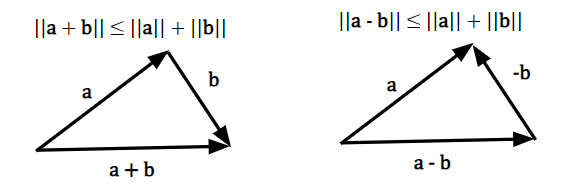
\includegraphics[scale=0.8]{assets/triangle_min_plu.png}
\end{center}

\section{Singular Value Decomposition \& Basic Applications (Section 4.1, 4.2)}
The singular value decomposition, known as \textbf{SVD}, is a matrix decomposition (similar to eigenvector, eigenvalues, but less restrictive). SVD is used for 
\begin{itemize}
    \item low rank approximation (imaging).
    \item least squares when rank is not full. 
\end{itemize}

\begin{theorem}{SVD Theorem}{}
    Let $A \in \R^{n \times m}$, with $A \neq 0$ and assume $n \geq m$ with $\text{rank}(A) = r \leq m$. Then, there exists orthogonal matrices $U \in \R^{n \times n}$ and $V \in \R^{m \times m}$ and positive numbers $\sigma_1 \geq \sigma_2 \geq \hdots \geq \sigma_r > 0$ such that \[A = U \Sigma V^T\] with \[\Sigma = \begin{bmatrix}
        \sigma_1 & 0 & 0 & 0 & 0 & \hdots & 0 \\ 
        0 & \sigma_2 & 0 & 0 & 0 & \hdots & 0 \\ 
        0 & 0 & \ddots & 0 & 0 & \hdots & 0 \\ 
        0 & 0 & 0 & \sigma_r & 0 & \hdots & 0 \\ 
        0 & 0 & 0 & 0 & 0 & \hdots & 0 \\ 
        \vdots & \vdots & \vdots & \vdots & \vdots & \ddots & \vdots \\ 
        0 & 0 & 0 & 0 & 0 & \hdots & 0
    \end{bmatrix} \in \R^{n \times m}.\]
    (Note that $\Sigma$ is a rectangular ``diagonal'' matrix.)
\end{theorem}
This is called a full SVD\footnote{Later, we will introduced a reduced SVD.} Here, $\sigma_1, \sigma_2, \hdots, \sigma_r$ are called the \emph{singular values}.

\textbf{Remarks:}
\begin{itemize}
    \item Notice that $A = U\Sigma V^T \implies AV = U\Sigma V^T V = U\Sigma$. If you compare this to eigenvectors and eigenvalues, you will notice that $AV = V\Lambda$. 
    
    \item The SVD is not unique. Instead of $U$, we can try $-U$; likewise, instead of $V$, we can use $-V$. 
\end{itemize}

\subsection{Other Forms of the SVD Theorem}

\begin{theorem}{Geometric Singular Value Decomposition Theorem}{}
    Let $A \in \R^{n \times m}$ be a nonzero matrix with rank $r$. Then, $\R^m$ has an orthonormal basis $v_1, v_2, \hdots, v_m$, $\R^n$ has an orthonormal basis $u_1, u_2, \hdots, u_n$, and there exists $\sigma_1 \geq \sigma_2 \geq \hdots \geq \sigma_r > 0$ such that 
    \[Av_i = \begin{cases}
        \sigma_i u_i & i = 1, \hdots, r \\ 
        \0 & i = r + 1, \hdots, m
    \end{cases} \qquad A^T u_i = \begin{cases}
        \sigma_i v_i & i = 1, \hdots, r \\ 
        \0 & i = r + 1, \hdots, n
    \end{cases}.\]
    For SVD, there exists orthogonal matrices $U \in \R^{n \times n}$ and $V \in \R^{m \times m}$ such that \[A = U \Sigma V^T\] with \[\Sigma = \begin{bmatrix}
        \sigma_1 & 0 & 0 & 0 & 0 & \hdots & 0 \\ 
        0 & \sigma_2 & 0 & 0 & 0 & \hdots & 0 \\ 
        0 & 0 & \ddots & 0 & 0 & \hdots & 0 \\ 
        0 & 0 & 0 & \sigma_r & 0 & \hdots & 0 \\ 
        0 & 0 & 0 & 0 & 0 & \hdots & 0 \\ 
        \vdots & \vdots & \vdots & \vdots & \vdots & \ddots & \vdots \\ 
        0 & 0 & 0 & 0 & 0 & \hdots & 0
    \end{bmatrix} \in \R^{n \times m}.\]
\end{theorem}
\textbf{Remarks:}
\begin{itemize}
    \item This is called a full SVD\footnote{Later, we will introduced a reduced SVD.} Here, $\sigma_1, \sigma_2, \hdots, \sigma_r$ are called the \emph{singular values}.
    \item Note that we can write $U$ and $V$ as a vector of vectors, 
    \[U = \begin{bmatrix}
        u_1, u_2, \hdots, u_n
    \end{bmatrix}, u_i \in \R^{n}\]
    and \[V = \begin{bmatrix}
        v_1, v_2, \hdots, v_m
    \end{bmatrix}, v_m \in \R^m.\]
\end{itemize}

\subsection{Intuition}
To get some intuition, let's suppose we start with $A = U\Sigma V^T$. Then, we know that \[AV = U\Sigma V^T V \implies AV = U\Sigma.\] Rewriting $V$ and $U$ as columns, we have 
\begin{equation}{\label{lec15:1}}
    A\begin{bmatrix}
        v_1 & v_2 & \hdots & v_m
    \end{bmatrix} = \begin{bmatrix}
        u_1 & u_2 & \hdots & u_n
    \end{bmatrix} \begin{bmatrix}
        \sigma_1 & 0 & 0 & 0 & 0 & \hdots & 0 \\ 
        0 & \sigma_2 & 0 & 0 & 0 & \hdots & 0 \\ 
        0 & 0 & \ddots & 0 & 0 & \hdots & 0 \\ 
        0 & 0 & 0 & \sigma_r & 0 & \hdots & 0 \\ 
        0 & 0 & 0 & 0 & 0 & \hdots & 0 \\ 
        \vdots & \vdots & \vdots & \vdots & \vdots & \ddots & \vdots \\ 
        0 & 0 & 0 & 0 & 0 & \hdots & 0
    \end{bmatrix}.
\end{equation}
For some matrix 
\[B = \begin{bmatrix}
    b_1 & b_2 & \hdots & b_m
\end{bmatrix},\] then \[B \begin{bmatrix}
    \sigma_1 & 0 & 0 & \hdots & 0 \\ 
    0 & 0 & 0 & \hdots & 0 \\ 
    0 & 0 & 0 & \hdots & 0 \\ 
    \vdots & \vdots & \vdots & \ddots & \vdots \\
    0 & 0 & 0 & \hdots & 0
\end{bmatrix} = \begin{bmatrix}
    b_1 & b_2 & \hdots & b_m
\end{bmatrix}\begin{bmatrix}
    \sigma_1 & 0 & 0 & \hdots & 0 \\ 
    0 & 0 & 0 & \hdots & 0 \\ 
    0 & 0 & 0 & \hdots & 0 \\ 
    \vdots & \vdots & \vdots & \ddots & \vdots \\
    0 & 0 & 0 & \hdots & 0
\end{bmatrix} = \begin{bmatrix}
    \sigma_1 b_1 & \0 & \hdots & \0
\end{bmatrix}.\]
Likewise, \[B \begin{bmatrix}
    0 & 0 & 0 & \hdots & 0 \\ 
    0 & \sigma_2 & 0 & \hdots & 0 \\ 
    0 & 0 & 0 & \hdots & 0 \\ 
    \vdots & \vdots & \vdots & \ddots & \vdots \\
    0 & 0 & 0 & \hdots & 0
\end{bmatrix} = \begin{bmatrix}
    b_1 & b_2 & \hdots & b_m
\end{bmatrix}\begin{bmatrix}
    0 & 0 & 0 & \hdots & 0 \\ 
    0 & \sigma_2 & 0 & \hdots & 0 \\ 
    0 & 0 & 0 & \hdots & 0 \\ 
    \vdots & \vdots & \vdots & \ddots & \vdots \\
    0 & 0 & 0 & \hdots & 0
\end{bmatrix} = \begin{bmatrix}
    \0 & \sigma_2 b_2 & \hdots & \0
\end{bmatrix}.\] 
Notice how $\sigma_i$ scales the $i$th column of $B$. Now, let's suppose we combine the operations above into one matrix: 
\[B \begin{bmatrix}
    \sigma_1 & 0 & 0 & \hdots & 0 \\ 
    0 & \sigma_2 & 0 & \hdots & 0 \\ 
    0 & 0 & 0 & \hdots & 0 \\ 
    \vdots & \vdots & \vdots & \ddots & \vdots \\
    0 & 0 & 0 & \hdots & 0
\end{bmatrix} = \begin{bmatrix}
    0 & b_2 & \hdots & 0
\end{bmatrix}\begin{bmatrix}
    \sigma_1 & 0 & 0 & \hdots & 0 \\ 
    0 & \sigma_2 & 0 & \hdots & 0 \\ 
    0 & 0 & 0 & \hdots & 0 \\ 
    \vdots & \vdots & \vdots & \ddots & \vdots \\
    0 & 0 & 0 & \hdots & 0
\end{bmatrix} = \begin{bmatrix}
    \sigma_1 b_1 & \sigma_2 b_2 & \hdots & \0
\end{bmatrix}.\] 
Here, both column 1 and 2 are scaled. So, going back to equation (\ref{lec15:1}), we have 
\[\begin{bmatrix}
    \sigma_1 u_1 & \sigma_2 u_2 & \hdots & \sigma_r u_r & \0 & \hdots & \0
\end{bmatrix}.\]
This gives us the formula,
\[Av_i = \begin{cases}
    \sigma_i u_i & i = 1, \hdots, r \\ 
    \0 & i = r + 1, \hdots, m
\end{cases}.\]

Likewise, let's consider $A^T$; 
\begin{equation*}
    \begin{aligned}
        A^T &= (U\Sigma V^T)^T \\ 
            &= (V^T) \Sigma^T U^T \\ 
            &= V\Sigma U^T.
    \end{aligned}
\end{equation*}
From there, we have $A^T U = V\Sigma^T U^T U = V\Sigma^T.$ Expanding out the matrices, we have 
\[A^T \begin{bmatrix}
    u_1 & u_2 & \hdots & u_n
\end{bmatrix} = \begin{bmatrix}
    v_1 & v_2 & \hdots & v_m
\end{bmatrix} \begin{bmatrix}
    \sigma_1 & 0 & 0 & \hdots & 0 \\ 
    0 & \sigma_2 & 0 & \hdots & 0 \\ 
    0 & 0 & \sigma_r & \hdots & 0 \\ 
    \vdots & \vdots & \vdots & \ddots & \vdots \\
    0 & 0 & 0 & \hdots & 0
\end{bmatrix} = \begin{bmatrix}
    \sigma_1 v_1 & \sigma_2 v_2 & \hdots & \sigma_r v_r & \0 & \hdots
\end{bmatrix}.\]
Note that $\Sigma^T$ is not a tall matrix, but a wide one; instead of being $n \times m$, it's $m \times n$. This gives us the formula
\[A^T u_i = \begin{cases}
    \sigma_i v_i & i = 1, \hdots, r \\ 
    \0 & i = r + 1, \hdots, m
\end{cases}.\] In particular, we can see that 
\begin{center}
    \begin{tabular}{p{2in} p{2in}}
        \[v_1 \xrightarrow[\sigma_1]{A} u_1\]
        \[v_2 \xrightarrow[\sigma_2]{} u_2\]
        \[v_3 \xrightarrow[\sigma_3]{} u_3\]
        \[\vdots\]
        \[v_r \xrightarrow[\sigma_r]{} u_r\]
        \[v_{r + 1} \xrightarrow{} \0\]
        \[\vdots\]
        \[v_{m} \xrightarrow{} \0\] &  
        \[u_1 \xrightarrow[\sigma_1]{A^T} v_1\]
        \[u_2 \xrightarrow[\sigma_2]{} v_2\]
        \[u_3 \xrightarrow[\sigma_3]{} v_3\]
        \[\vdots\]
        \[u_r \xrightarrow[\sigma_r]{} v_r\]
        \[u_{r + 1} \xrightarrow{} \0\]
        \[\vdots\]
        \[u_{n} \xrightarrow{} \0\]
    \end{tabular}
\end{center}
So, in particular, the range of matrix A, $\mathcal{R}(A)$, is spanned by 
\[v_1 \xrightarrow[\sigma_1]{A} u_1\]
\[v_2 \xrightarrow[\sigma_2]{} u_2\]
\[v_3 \xrightarrow[\sigma_3]{} u_3\]
\[\vdots\]
\[v_r \xrightarrow[\sigma_r]{} u_r.\]
The null space of $A$, $\mathcal{N}(A)$, is spanned by 
\[v_{r + 1} \xrightarrow{} \0\]
\[\vdots\]
\[v_{m} \xrightarrow{} \0.\]
For $A^T$, this is analogous.

\subsection{Fundamental Subspaces}
The SVD displays orthogonal bases for the four Fundamental subspaces, $\mathcal{R}(A)$, $\mathcal{N}(A)$, $\mathcal{R}(A^T)$, and $\mathcal{N}(A^T)$, where $\mathcal{R}$ is the \emph{range} and $\mathcal{N}$ is the null space. 
\[\mathcal{R}(A) = \text{span}\{u_1, u_2, \hdots, u_r\}.\]
\[\mathcal{N}(A) = \text{span}\{v_{r + 1}, v_{r + 2}, \hdots, v_m\}.\]
\[\mathcal{R}(A^T) = \text{span}\{v_1, v_2, \hdots, v_r\}.\]
\[\mathcal{N}(A^T) = \text{span}\{u_{r + 1}, u_{r + 2}, \hdots, u_n\}.\]
In particular, 
\[\mathcal{R}(A) + \mathcal{N}(A^T) = \text{span}\{u_1, u_2, \hdots, u_n\}.\]
\[\mathcal{R}(A^T) + \mathcal{N}(A) = \text{span}\{v_1, v_2, \hdots, v_m\}.\]
We can see that $\mathcal{R}(A^T) = \mathcal{N}(A)^{\perp}$ and $\mathcal{R}(A) = \mathcal{N}(A^T)^{\perp}.$

\begin{corollary}{}{}
    Let $A \in \R^{n \times m}$. Then, $\dim(\mathcal{R}(A)) + \dim(\mathcal{N}(A)) = m$ and $\dim(\mathcal{R}(A^T)) + \dim(\mathcal{N}(A^T)) = n$.
\end{corollary}

\subsection{Reduced SVD}
We'll introduce this section with an example. 

\begin{mdframed}
    (Example.) Suppose we have a $3 \times 3$ matrix of rank\footnote{It has 3 rows but only has 2 non-zero singular values, $\sigma_1$ and $\sigma_2$} 2. Then, 
    \begin{equation*}
        \begin{aligned}
            A &= \underbrace{\begin{bmatrix}
                u_{11} & u_{12} & u_{13} \\ 
                u_{21} & u_{22} & u_{23} \\ 
                u_{31} & u_{32} & u_{33} 
            \end{bmatrix}}_{U} \underbrace{\begin{bmatrix}
                \sigma_1 & 0 & 0 \\ 
                0 & \sigma_2 & 0 \\ 
                0 & 0 & 0 
            \end{bmatrix}}_{\Sigma} \underbrace{\begin{bmatrix}
                v_{11} & v_{21} & v_{31} \\ 
                v_{12} & v_{22} & v_{32} \\ 
                v_{13} & v_{23} & v_{33} 
            \end{bmatrix}}_{V^T} \\ 
                &= \begin{bmatrix}
                    \sigma_1 u_{11} & \sigma_2 u_{12} & 0 \\ 
                    \sigma_1 u_{21} & \sigma_2 u_{22} & 0 \\ 
                    \sigma_1 u_{31} & \sigma_2 u_{32} & 0 
                \end{bmatrix} \begin{bmatrix}
                    v_{11} & v_{21} & v_{31} \\ 
                    v_{12} & v_{22} & v_{32} \\ 
                    v_{13} & v_{23} & v_{33} 
                \end{bmatrix}.
        \end{aligned}
    \end{equation*} 
    As a result, we'll end up multiplying $v_{13}$, $v_{23}$, $v_{33}$ by 0. So, instead, what if we have: 
    \[A = \underbrace{\begin{bmatrix}
        u_{11} & u_{12} \\ 
        u_{21} & u_{22} \\ 
        u_{31} & u_{32} 
    \end{bmatrix}}_{\hat{U}} \underbrace{\begin{bmatrix}
        \sigma_1 & 0 \\ 
        0 & \sigma_2
    \end{bmatrix}}_{\hat{\Sigma}} \underbrace{\begin{bmatrix}
        v_{11} & v_{21} & v_{31} \\ 
        v_{12} & v_{22} & v_{32}
    \end{bmatrix}}_{\hat{V^T}}.\]
    This is known as the reduced SVD. 
\end{mdframed}

\begin{theorem}{Condensed SVD Theorem}{}
    Let $A \in \R^{n \times m}$ be a nonzero matrix of rank $r$. Then, there exists $\hat{U} \in \R^{n \times r}$, $\hat{\Sigma} \in \R^{r \times r}$, and $\hat{V} \in \R^{m \times r}$, such that $\hat{U}$ and $\hat{V}$ are isometries, and $\hat{\Sigma}$ is a diagonal matrix with main-diagonal entries $\sigma_1 \geq \sigma_2 \geq \hdots \geq \sigma_r > 0$ and \[A = \hat{U}\hat{\Sigma}\hat{V^T}.\]
\end{theorem}


\subsection{Relationship to Norm and Condition Number}
Recall that we defined the matrix 2-norm as  
\[||A|| = \max_{\x \neq \0} \frac{||A\x||_2}{||\x||} = \sigma_1,\] where $\sigma_1$ is the largest singular value. Note that this definition also makes sense for $A \in \R^{n \times m}$. 

\begin{theorem}{}{}
    \[||A||_2 = \sigma_1.\]
\end{theorem}

Since $A$ and $A^T$ have the same singular values, we have the following corollary. 
\begin{corollary}{}{}
    \[||A||_2 = ||A^T||_2.\]
\end{corollary}
Since $A$ is nonsingular, $A$ has full rank, i.e., rank $n$. $A$ has $n$ strictly positive singualr values, $\sigma_1 \geq \sigma_2 \geq \hdots \geq \sigma_n > 0$. Now, 
\[A^{-1} Av_i = A^{-1}(\sigma_i u-i) \implies v_i = \sigma_i A^{-1} u_i \implies A^{-1} u_i = \frac{1}{\sigma_i} v_i,\] so in particular we can map each $\sigma$ like so: 
\begin{center}
    \begin{tabular}{p{2in} p{2in}}
        \[A\] & \[A^{-1}\] \\ 
        \[v_1 \xrightarrow[\sigma_1]{} u_1\]
        \[v_2 \xrightarrow[\sigma_2]{} u_2\]
        \[v_3 \xrightarrow[\sigma_3]{} u_3\]
        \[\vdots\]
        \[v_n \xrightarrow[\sigma_n]{} u_n\] &
        \[u_1 \xrightarrow[\sigma_1^{-1}]{} v_1\]
        \[u_2 \xrightarrow[\sigma_2^{-1}]{} v_2\]
        \[u_3 \xrightarrow[\sigma_3^{-1}]{} v_3\]
        \[\vdots\]
        \[u_{n} \xrightarrow[\sigma_n^{-1}]{} v_n\]
    \end{tabular}
\end{center}
This tells us that the singular values of $A^{-1}$ must be \[\frac{1}{\sigma_n} \geq \frac{1}{\sigma_{n - 1}} \geq \hdots \geq \frac{1}{\sigma_2} \geq \frac{1}{\sigma_1} > 0\]
such that 
\[\Sigma^{-1} = \begin{bmatrix}
    \frac{1}{\sigma_1} & 0 & 0 & 0 \\ 
    0 & \frac{1}{\sigma_2} & 0 & 0 \\ 
    0 & 0 & \ddots & 0 \\ 
    0 & 0 & 0 & \frac{1}{\sigma_n} 
\end{bmatrix}.\]
And, in particular, \[||A^{-1}||_2 = \frac{1}{\sigma_n} \qquad ||A||_2 = \sigma_1.\]

\begin{theorem}{}{}
    Let $A \in \R^{n \times n}$ be a nonsingular matrix with singular values $\sigma_1 \geq \hdots \geq \sigma_n > 0$. Then, 
    \[\kappa_{2}(A) = \frac{\sigma_1}{\sigma_n}.\]
\end{theorem}

\subsection{More on SVD}
Remember that there are two types of SVD: 
\begin{itemize}
    \item Full SVD.
    \[A = U\Sigma V^T,\]
    where $A$ is $n \times m$, $U$ is $n \times n$, $\Sigma$ is $n \times m$, and $V^T$ is $m \times m$. Here, $\text{rank}(A) = r \leq m$ and $n \geq m$. 

    \item Reduced SVD 
    \[A = \hat{U}\hat{\Sigma}\hat{V^T},\]
    where $A$ is $n \times m$, $\hat{U}$ is $n \times r$, $\hat{\Sigma}$ is $r \times r$, and $\hat{V}^T$ is $r \times m$.
\end{itemize}
In any case, we now know that \[||A||_2 = \sigma_1 \qquad \kappa_{2}(A) = \frac{\sigma_1}{\sigma_n}.\]

\subsection{Rank-1 Decomposition}
\begin{theorem}{}{}
    Let $A \in \R^{n \times m}$ be a nonzero matrix with rank $r$. Let $\sigma_1, \hdots, \sigma_r$ be the singular values of $A$, with associated right and left singular vectors $v_1, \hdots, v_r$ and $u_1, \hdots, u_r$, respectively. Then, 
    \[A = \sum_{j = 1}^{r} \sigma_j u_j v_j^T,\]
    where $u_j \in \R^{n}$, $v_j \in \R^{m}$, and $u_j v_j^T \in \R^{n \times m}$. 
\end{theorem}
To see why this theorem works, 
\begin{equation*}
    \begin{aligned}
        A &= \hat{U}\hat{\Sigma}\hat{V^T} \\ 
            &= \underbrace{\begin{bmatrix}
                u_1 & v_2 & \hdots & u_r
            \end{bmatrix}}_{\hat{U}} \underbrace{\begin{bmatrix}
                \sigma_1 & 0 & 0 & 0 \\ 
                0 & \sigma_2 & 0 & 0 \\ 
                0 & 0 & \ddots & 0 \\ 
                0 & 0 & 0 & \sigma_r
            \end{bmatrix}}_{\hat{\Sigma}} \underbrace{\begin{bmatrix}
                v_1^T \\ v_2^T \\ \vdots \\ v_r^T
            \end{bmatrix}}_{\hat{V}} \\ 
            &= \begin{bmatrix}
                \sigma_1 u_1 & \sigma_2 u_2 & \hdots & \sigma_r u_r
            \end{bmatrix} \begin{bmatrix}
                v_1^T \\ v_2^T \\ \vdots \\ v_r^T
            \end{bmatrix} \\ 
            &= \sigma_1 u_1 v_1^T + \sigma_2 u_2 v_2^T + \hdots + \sigma_r u_r v_r^T \\ 
            &= \sum_{i = 1}^{r} \sigma_i u_i v_{i}^T.
    \end{aligned}
\end{equation*}
This is called the \textbf{rank-1 decomposition} because $A$ is written as a sum of rank-1 matrices ($u_i v_i^T$ is a rank-1 matrix.)

\subsubsection{Low Rank Approximation}
We know that \[A = \sum_{i = 1}^{r} \sigma_i u_i v_i^T = \sigma_1 u_1 v_1^T + \sigma_2 u_2 v_2^T + \hdots + \sigma_r u_r v_r^T.\] We also know that $\sigma_1 \geq \sigma_2 \geq \hdots \geq \sigma_r$. So, we can choose some $k \leq r$ and define \[A_k = \sum_{i = 1}^{k} \sigma_i u_i v_i^T.\] Then, $A_k$ is called the rank-$k$ approximation of $A$ (it's of type ``low-rank'' when $k < r$). 

\bigskip 

Essentially, we cut-off parts of the sum belonging to small singular values, producing an approximation ($A_k$) to the original matrix ($A$). It should, then, be noted that $\text{rank}(A_k) = k$, with each $u_i v_i^T$ having rank 1. 

\begin{theorem}{}{}
    \[||A - A_k||_2 = \sigma_{k + 1}.\]
\end{theorem}

\begin{proof}
    We know that $A = \hat{U}\hat{\Sigma}\hat{V}^T$ and $A_k = \hat{U}\hat{\Sigma}_k \hat{V}^T$. So, \[\hat{\Sigma} = \begin{bmatrix}
        \sigma_1 & & &  \\ 
        & \sigma_2 & & \\ 
        & & \ddots & \\ 
        & & & \sigma_r
    \end{bmatrix} \qquad \hat{\Sigma}_k = \begin{bmatrix}
        \sigma_1 & & &  \\ 
        & \ddots & & \\ 
        & & \sigma_k & \\ 
        & & & 0 
    \end{bmatrix}.\]
    From this, \[\begin{aligned}
        A - A_k &= \hat{U}(\hat{\Sigma} - \hat{\Sigma}_k) \hat{V}^T \\ 
            &= \hat{U}\begin{bmatrix}
                0 & & & & & & \\ 
                & 0 & & & & & \\ 
                & & \ddots & & & & \\ 
                & & & 0 & & & \\ 
                & & & & \sigma_{k + 1} & & \\ 
                & & & & & \ddots & \\ 
                & & & & & & \sigma_r
            \end{bmatrix} \hat{V}^T
    \end{aligned},\]
    as desired.
\end{proof}
In addition, $A_k$ is the matrix of rank $k$ that is closest to $A$ (in the 2-norm). In other words, $\min||A - B||_2$ with minimum over all matrix $B$ of rank $k$ is $A_k$. 


\section{Pseudoinverse (Section 4.3)}
We will solve the least squares with the SVD with full rank matrix $A$. Using SVD also works when the rank of $A$ is not full. Recall that 
\[A \in \R^{n \times m} \qquad n \geq m \qquad \min_{\x \in \R^m} ||\b - A\x||_2^2.\]

\subsection{Brief Review}
Recall that, for a full rank $A$, i.e., $\text{rank}(A) = m$, we can use full QR decomposition ($A = QR$) or reduced QR decomposition ($A = \hat{Q}\hat{R}$). In particular, for reduced QR, $A = \hat{Q}\hat{R}$ where $\hat{Q} \in \R^{n \times m}$ and $\hat{R} \in \R^{m \times m}$. Recall that $A\x = \b$ as well, so 
\begin{equation*}
    \begin{aligned}
        A\x &= \b \\ 
            &\implies \hat{Q}\hat{R}\x = \b \\ 
            &\implies \hat{Q}^{T}\hat{Q}\hat{R}\x = \hat{Q}^{T}\b \\ 
            &\implies \hat{R}\x = \hat{Q}^{T}\b && \text{Since } Q^T Q = I.
    \end{aligned}
\end{equation*}
Remember that, because $\hat{Q}$ is orthogonal, $\hat{Q} \hat{Q}^T = I_{n \times n}$ and $\hat{Q}^T \hat{Q} = I_{m \times m}$. Now, remember that if $\hat{R}$ has full rank, then it'll look like 
\[\hat{R} = \begin{bmatrix}
    * & * & * & * & \hdots & * \\ 
    0 & * & * & * & \hdots & * \\ 
    0 & 0 & * & * & \hdots & * \\ 
    0 & 0 & 0 & * & \hdots & * \\ 
    \vdots & \vdots & \vdots & \vdots & \ddots & \vdots \\ 
    0 & 0 & 0 & 0 & \hdots & * \\ 
\end{bmatrix}.\]
Then, the associated equation will have a unique solution since it has $m$ equations and $m$ unknowns. \textbf{Now}, what if $\text{rank}(R) = r < m$? Then, it is not full rank and it'll look like 
\[\hat{R} = \begin{bmatrix}
    * & * & * & * & \hdots & * \\ 
    0 & * & * & * & \hdots & * \\ 
    0 & 0 & * & * & \hdots & * \\ 
    0 & 0 & 0 & 0 & \hdots & 0 \\ 
    \vdots & \vdots & \vdots & \vdots & \ddots & \vdots \\ 
    0 & 0 & 0 & 0 & \hdots & 0 \\ 
\end{bmatrix}.\]
In particular, some of the diagonal entries are 0's. So, $\hat{R}\x = \hat{Q}^T \b$. We have $m$ unknowns, but we only have $r$ independent equations. Those equations are not helpful since we can't use them to solve for the unknowns -- we'll end up with infinitely many solutions. So, we'll have to choose one of these infinitely many solutions based on $||\x||_2$. 

\subsection{A New Problem}
We now have a new problem to solve. 
\begin{itemize}
    \item Find $\min||\b - A\x||_2^2$ (infinitely many solutions.)
    \item Pick $\x$ with minimal $||\x||_2$. 
\end{itemize}
With the above two minimizers, there \emph{will} be a unique solution $\x$. We will see that the unique $\x$ can be written as $\x = A^+ \b$, where $A^+$ is known as the \textbf{pseudoinverse}\footnote{Note that if $A$ is invertible, then $\x = A^{-1}\b$, so in some sense $A^+$ is mimicking $A^{-1}$.}.

\bigskip 

With this in mind, how do we find the least squares solution of the minimal 2-norm? With $A = U\Sigma V^T$, we have 
\begin{equation*}
    \begin{aligned}
        ||\b - A\x||_2^2 &= ||\b - U\Sigma V^T \x||_2^2 \\ 
            &= ||U(U^T \b) - U(\Sigma V^T \x)||_2^2 && \text{Recall that } UU^T = U^T U = I \\ 
            &= ||U(U^T \b - \Sigma V^T \x)||_2^2 \\ 
            &= ||U^T \b - \Sigma V^T \x||_2^2 \\ 
            &= \left|\left| \underbrace{\begin{bmatrix}
                \hat{c} \\ 
                d
            \end{bmatrix}}_{U^T \b \in \R^{n \times 1}} - \left[
                \begin{array}{c|c}
                    \hat{\Sigma} & \makebox{0} \\ 
                    \hline 
                    \makebox{0} & \makebox{0}
                \end{array}
            \right] \underbrace{\begin{bmatrix}
                \hat{y} \\ z
            \end{bmatrix}}_{V^T \x \in \R^{m \times 1}} \right|\right|_2^2 && \text{See remark.} \\ 
            &= \left|\left| \begin{bmatrix}
                \hat{c} \\ 
                d
            \end{bmatrix} - \begin{bmatrix}
                \hat{\Sigma} \hat{y} \\ 
                \0
            \end{bmatrix} \right|\right|_2^2  \\ 
            &= \left|\left| \begin{bmatrix}
                \hat{c} - \hat{\Sigma} \hat{y} \\ 
                d
            \end{bmatrix} \right|\right|_2^2 \\ 
            &= ||\hat{c} - \hat{\Sigma} \hat{y}||_2^2 + ||d||_2^2
    \end{aligned}
\end{equation*}
\textbf{Remarks:}
\begin{itemize}
    \item Note that $\hat{c} \in \R^r$ and $d \in \R^{n - r}$ and $\hat{y} \in \R^r$ and $z \in \R^{m - r}$.
    \item Additionally, \[\Sigma = \left[
        \begin{array}{c|c}
            \hat{\Sigma} & \makebox{0} \\ 
            \hline 
            \makebox{0} & \makebox{0}
        \end{array}
    \right]\] where $\hat{\Sigma}$ is an $r \times r$ matrix. 

    \item $d$ is independent of $\x$ when minimizing over $\x$. 
\end{itemize}
In any case, we want to minimize $||\hat{c} - \hat{\Sigma} \hat{y}||_2^2$. This can be done by solving \[\hat{c} = \hat{\Sigma}\hat{y}.\] This yields \[\begin{bmatrix}
    \sigma_1 & & & & \\ 
    & \sigma_2 & & & \\ 
    & & \sigma_3 & & \\ 
    & & & \ddots & \\ 
    & & & & \sigma_r
\end{bmatrix} \begin{bmatrix}
    \hat{y}_1 \\ \hat{y}_2 \\ \vdots \\ \hat{y}_r
\end{bmatrix} = \begin{bmatrix}
    \hat{c}_1 \\ \hat{c}_2 \\ \vdots \\ \hat{c}_r
\end{bmatrix}.\]
And this gives us 
\[\hat{y}_i = \frac{\hat{c}_i}{\sigma_i}, i = 1, \hdots, r.\] To find $\x$, we do \[V^T \x = \begin{bmatrix}
    \hat{y} \\ z
\end{bmatrix} \implies \x = V\begin{bmatrix}
    \hat{y} \\ z 
\end{bmatrix}.\]
No matter the value of $z$, it won't affect the value of $\hat{y}$. We can define many $\x$ values such that the least square problems has the minimum. However, we want to define the unique solution $\x$, so how do we choose $z$ so we can find the minimized $||\x||_2$? 
\[||\x||_2^2 = \left|\left|V \begin{bmatrix}
    \hat{y} \\ z
\end{bmatrix}\right|\right|_2^2 = \left|\left|\begin{bmatrix}
    \hat{y} \\ 
    z
\end{bmatrix}\right|\right|_2^2 = ||\hat{y}||_2^2 + ||z||_2^2,\] where recall that $V$ is orthogonal. So, $||\x||_2^2$ is minimized when $z = \0$. So, in summary, $\boxed{\x = V\begin{bmatrix}
    \hat{y} \\ \0
\end{bmatrix}}$ is the unique solution.







\section{Eigenvector and Eigenvalues (Section 5.1, 5.2)}
Fundamentally, we want to solve \begin{equation}{\label{eq:2-27:1}}
    Av = \lambda v,
\end{equation} where
\begin{itemize}
    \item $A$ is a matrix either in $\R^{n \times n}$ or $\C^{n \times n}$, and 
    \item $\lambda \in \C$ (the \emph{eigenvalue}), and 
    \item $v \in \C^n$ (the \emph{eigenvector}).
\end{itemize}
The pair $(\lambda, v)$ is called an \textbf{eigenpair} of $A$. Whereas each eigenvector has a unique eigenvalue associated with it, each eigenvalue is associated with many eigenvectors. For example, if $v$ is an eigenvector of $A$ associated with the eigenvalue $\lambda$, then every nonzero multiple of $v$ is also an eigenvector of $A$ associated with $\lambda$. Now, note that 
\[Av = \lambda v \implies Av = \lambda I v \implies \0 = Av - \lambda I v \implies  \0 = (A - \lambda I)v,\]
where $I$ is the $n \times n$ identity matrix. In any case, if $v$ is an eigenvector with eigenvalue $\lambda$, then $v$ is a nonzero solution of the homogeneous matrix equation \[(A - \lambda I)v = \0.\] Therefore, the matrix is singular\footnote{Not invertible.} and $\det(A - \lambda I) = 0$. This establishes the following theorem. 

\begin{theorem}{}{2-27:2}
    $\lambda$ is an eigenvalue of $A$ if and only if 
    \[\det(A - \lambda I) = 0.\]
    This equation is known as the \textbf{characteristic equation} of $A$.
\end{theorem}
\textbf{Remark:} Although this is useful theoretically, this equation has little value for actual computations, as we will see later. 

We note that $\det(A - \lambda I)$ is a polynomial in $\lambda$ of degree $n$; it is called the \textbf{characteristic polynomial} of $A$. Therefore, the eigenvalues, $\lambda$, are the roots of this polynomial. There are exactly $n$ roots, not all real (i.e., some complex), and thus $n$ eigenvalues.

\begin{mdframed}
    (Exercise.) Find the characteristic polynomial of \[B = \begin{bmatrix}
        1 & 2 \\ 3 & 4
    \end{bmatrix}.\]

    \begin{mdframed}
        We have 
        \begin{equation*}
            \begin{aligned}
                \det(B - \lambda I) &= \det\left(\begin{bmatrix}
                    1 & 2 \\ 3 & 4
                \end{bmatrix} - \lambda \begin{bmatrix}
                    1 & 0 \\ 0 & 1
                \end{bmatrix}\right) \\ 
                    &= \det\left(\begin{bmatrix}
                        1 - \lambda & 2 \\ 
                        3 & 4 - \lambda
                    \end{bmatrix}\right) \\ 
                    &= (1 - \lambda)(4 - \lambda) - 3(2) \\ 
                    &= 4 - \lambda - 4\lambda + \lambda^2 - 6 \\ 
                    &= \lambda^2 - 5\lambda - 2.
            \end{aligned}
        \end{equation*}
    \end{mdframed}
\end{mdframed}

\subsection{Getting Eigenvectors}
We can get the eigenvectors by solving \begin{equation}{\label{eq:2-27:3}}
    (A - \lambda I)v = \0,
\end{equation}
where $\lambda$ are the eigenvalues that we found by solving (\ref{th:2-27:2}). Note that 
\begin{itemize}
    \item Eigenvalues are the roots of the polynomials of (\ref{th:2-27:2}).
    \item Roots can be complex, thus eigenvalues can also be complex \emph{even} when $A$ is real. 
\end{itemize}

\begin{mdframed}
    (Example.) Consider \[A = \begin{bmatrix}
        0 & -1 \\ 1 & 0
    \end{bmatrix} \in \R^{2 \times 2}.\] 
    \begin{itemize}
        \item To find the eigenvalues, we have 
        \[\det(A - \lambda I) = \det\left(\begin{bmatrix}
            -\lambda & -1 \\ 1 & -\lambda
        \end{bmatrix}\right) = \lambda^2 + 1.\]
        Then, we can solve \[\lambda^2 + 1 = 0,\] giving us $\lambda = \pm i$, which is \emph{complex}.  

        \item To find the eigenvectors, we use the formula (\ref{eq:2-27:3}) for each eigenvalue.
        \begin{itemize}
            \item For $\lambda = i$, we have 
            \[\left(\begin{bmatrix}
                0 & - 1 \\ 1 & 0 
            \end{bmatrix} - \begin{bmatrix}
                i & 0 \\ 
                0 & i
            \end{bmatrix}\right)v = \0 \implies \begin{bmatrix}
                -i & -1 \\ 
                1 & -i
            \end{bmatrix}v = \0 \implies v = \begin{bmatrix}
                i \\ 1
            \end{bmatrix}.\]
            
            \item For $\lambda = -i$, we have 
            \[\left(\begin{bmatrix}
                0 & -1 \\ 1 & 0
            \end{bmatrix} - \begin{bmatrix}
                -i & 0 \\ 
                0 & -i
            \end{bmatrix}\right)v = \0 \implies \begin{bmatrix}
                i & -1 \\ 1 & i
            \end{bmatrix}v = \0 \implies v = \begin{bmatrix}
                -i \\ 1
            \end{bmatrix}.\]
        \end{itemize}
    \end{itemize}
\end{mdframed}

\subsection{Eigenvectors \& Eigenvalues for Large Matrices}
Suppose we have a matrix of size $200 \times 200$. The characteristic equation will be a polynomial of degree 200. This means that there are 200 roots and thus 200 eigenvalues. Now, we should note that there is no formula to find the roots when $r > 4$ (we have the quadratic equation when $r = 2$, for example), so this process is tedious. Additionally, numerically finding the roots is ill-conditioned\footnote{Small perturbations to the coefficients lead to large changes in the roots.}.

\bigskip 

So, how do we find the eigenvalues numerically? As implied earlier, the characteristic equation is not useful for finding eigenvalues numerically, so we will perform iterative methods to find eigenvalues. 

\subsubsection{QR Iteration}
Before we begin this section, let's note a theorem. 
\begin{theorem}{}{}
    Let $T \in \C^{n \times n}$ be a (lower- or upper-) triangular matrix. Then, the eigenvalues of $T$ are the main-diagonal entries $t_{11}, \hdots, t_{nn}$. 
\end{theorem}
We will construct a sequence of matrices with the same eigenvalues that converge to a triangular matrix. The reason why we choose a triangular matrix is because its eigenvalues are on the diagonal. 

\subsection{Semisimple Matrices}
\begin{definition}{Semisimple Matrix}{}
    A matrix $A \in \R^{n \times n}$ is called \textbf{semisimple} if it has $n$ linearly independent eigenvectors. Otherwise, it is called \textbf{defective.}
\end{definition}

\begin{mdframed}
    (Example.) Consider \[I = \begin{bmatrix}
        1 & 0 \\ 0 & 1
    \end{bmatrix}.\] Its characteristic polynomial is given by \[\det(I - \lambda I) = (1 -\lambda)^2.\] Solving $(1 - \lambda)^2 = 0$ yields $\lambda_1 = \lambda_2 = 1$. So, we find $v_1 = \begin{bmatrix}
        1 \\ 0
    \end{bmatrix}$ and $v_2 = \begin{bmatrix}
        0 \\ 1
    \end{bmatrix},$ which are are linearly independent, which means that $I$ is semisimple.
\end{mdframed}
\textbf{Remark:} Any vector, except $\0$, can be an eigenvector.

\begin{mdframed}
    (Example.) Consider \[A = \begin{bmatrix}
        1 & 3 \\ 0 & 1
    \end{bmatrix}.\] Its characteristic polynomial is given by \[\det(A - \lambda I) = \det\left(\begin{bmatrix}
        1 - \lambda & 3 \\ 0 & 1 - \lambda
    \end{bmatrix}\right) = (1 - \lambda)^2.\] Solving $(1 - \lambda)^2 = 0$ yields $\lambda_1 = \lambda_2 = 1$. To get the eigenvectors, we solve \[(A - \lambda I)v = \0,\] so in particular \[\left(\begin{bmatrix}
        1 & 3 \\ 0 & 1
    \end{bmatrix} - 1 \cdot \begin{bmatrix}
        1 & 0 \\ 0 & 1
    \end{bmatrix}\right)v = \0 \implies \begin{bmatrix}
        0 & 3 \\ 0 & 0
    \end{bmatrix} \begin{bmatrix}
        v_1 \\ v_2
    \end{bmatrix} = \0 \implies \begin{cases}
        0v_1 + 3v_2 = 0 \\ 
        0v_1 + 0v_2 = 0
    \end{cases}.\] We find that $3v_2 = 0 \implies v_2 = 0$ and $v_1$ can be any arbitrary value \emph{except} 0 (because eigenvectors cannot be $\0$). In particular, every vector of the form \[v = \begin{bmatrix}
        v_1 \\ 0 
    \end{bmatrix} = v_1 \begin{bmatrix}
        1 \\ 0
    \end{bmatrix}\] is an eigenvector. However, this implies that there is only one linearly independent eigenvector hence $A$ is defective.
\end{mdframed}

\subsubsection{Reminders}
Recall that 
\begin{itemize}
    \item if $v$ is an eigenvector of $A$ with respect to $\lambda$, then $cv$ for some $c \in \R \setminus \{0\}$ is also an eigenvector of $A$ with respect to $\lambda$. In particularm 
    \[A(cv) = c(Av) = c(\lambda v) = \lambda(cv) \implies A(cv) = \lambda(cv).\]

    \item if $v$ is an eigenvector of $A$ with respect to $\lambda$, then $v$ is also an eigenvector of $A^{-1}$ with respect to $\lambda^{-1}$. 
    \[Av = \lambda v \implies A^{-1}(Av) = A^{-1}(\lambda v) \implies v = \lambda A^{-1}v \implies \lambda^{-1} v = A^{-1} v.\]
\end{itemize}
This brings us to another theorem. 
\begin{theorem}{}{}
    If $\lambda_1, \lambda_2, \hdots, \lambda_k$ are distinct eigenvalues of $A$, then the associated eigenvectors $v_1, v_2, \hdots, v_k$ are linearly independent. 
\end{theorem}




\section{The Power Method (Section 5.3)}
Let $A \in \C^{n \times n}$, and assume that $A$ is semisimple. Let $\lambda_1, \lambda_2, \hdots, \lambda_n$ denote the eigenvalues associated with the linearly independent eigenvectors, $v_1, \hdots, v_n$, respectively. Assume that the vectors are ordered so that $|\lambda_1| \geq |\lambda_2| \geq \hdots \geq |\lambda_n|$. If $|\lambda_1| > |\lambda_2|$, then $\lambda_1$ is called the \textbf{dominant eigenvalue}\footnote{Basically, the largest absolute eigenvalue.} and $v_1$ is called the \textbf{dominant eigenvector} of $A$.  

\subsection{The Iterative Power Method}
Assuming we have $|\lambda_1| > |\lambda_2|$ as described above (otherwise, this method may not work), the general idea behind the iterative power method is that we can pick $q \in \R^n$ randomly. Then, we can form the sequence of vectors
\[q, Aq, A^2 q, A^3 q, \hdots.\]
To calculate this sequence, we don't necessarily need to form the powers of $A$ explicitly. Each vector in the sequence can be obtained by multiplying the previous vector by $A$, e.g., $A^{j + 1}q = A(A^j q)$. It's easy to show that the sequence converge, in a sense, to a dominant eigenvector, for almost all choices of $q$. Since $v_1, \hdots, v_n$ form a basis for $\C^n$, there exists constants $c_1, \hdots, c_n$ such that  
\[q = c_1 v_1 + c_2 v_2 + \hdots + c_n v_n.\]
We don't know what $v_1, \hdots, v_n$ are, so we don't know what $c_1, \hdots, c_n$ are, either. However, it's clear that, for any choice of $q$, $c_1$ will be nonzero. The argument that follows is valid for every $q$ for which $c_1 \neq 0$; multiplying by $A$, we have 
\begin{equation*}
    \begin{aligned}
        Aq &= c_1 Av_1 + c_2 Ac_2 + \hdots + c_n Av_n \\ 
            &= c_1 \lambda_1 v_1 + c_2 \lambda_2 v_2 + \hdots + c_n  \lambda_n v_n.
    \end{aligned}
\end{equation*}
Similarly, 
\begin{equation*}
    \begin{aligned}
        A^2 q &= A(c_1 \lambda_1 v_1 + c_2 \lambda_2 v_2 + \hdots + c_n  \lambda_n v_n) \\
            &= c_1 \lambda_1 (Av_1) + c_2 \lambda_2 (Av_2) + \hdots + c_n \lambda_n (Av_n) \\ 
            &= c_1 \lambda_1 (\lambda_1 v_1) + c_2 \lambda_2 (\lambda_2 v_2) + \hdots + c_n \lambda_n (\lambda_n v_n) \\ 
            &= c_1 \lambda_1^2 v_1 + c_2 \lambda_2^2 v_2 + \hdots + c_n \lambda_n^2 v_n.
    \end{aligned}
\end{equation*}
In general, we have 
\begin{equation*}
    \begin{aligned}
        A^j q &= c_1 \lambda_1^j v_1 + c_2 \lambda_2^j v_2 + \hdots + c_n \lambda_n^j v_n \\ 
            &= \lambda_1^j \left(c_1 v_1 + c_2 \left(\frac{\lambda_2}{\lambda_1}\right)^j v_2 + \hdots + c_n \left(\frac{\lambda_n}{\lambda_1}\right)^j v_n\right).
    \end{aligned}
\end{equation*}
So, 
\[\frac{1}{\lambda_1^j} A^i q = c_1 v_1 + c_2 \left(\frac{\lambda_2}{\lambda_1}\right)^j v_2 + \hdots + c_n \left(\frac{\lambda_n}{\lambda_1}\right)^j v_n.\]
Notice that $\lim_{j \mapsto \infty} \left(\frac{\lambda_i}{\lambda_1}\right)^j = 0$ (because $|\lambda_1| > |\lambda_2| \geq |\lambda_3| \geq \hdots \geq |\lambda_n|$), so \[\lim_{j \mapsto \infty} \frac{1}{\lambda_1^j} A^j q = c_1 v_1,\]
the dominant eigenvector.

\bigskip 

\textbf{Remark:} In fact, when we use the power method to converge to a dominant eigenvector, we need to know all the eigenvalues and then check whether they're strictly greater or not. So, this only works if $\lambda_1$ is known and it is strictly greater than $\lambda_2$ and so on. 

\subsection{Scaling}
Notice how we went from $A_j q$ to $\frac{1}{\lambda_1^j} A^j q$? In some sense, we can say we're scaling $A_j q$. Now, what if we don't know what the value of $\lambda_1$ is, but we need to do \emph{some} scaling to get a reasonable convergence? In this case, we can still do some scaling, but not necessarily with $\lambda_1$. 

\bigskip 

Let's start with a random $q \in \R^n$; let $q_0 = q$. We want to use the iterative power formula method, 
\[\boxed{q_{j + 1} = \frac{1}{s_{j + 1}} Aq_j \qquad j = 0, 1, 2, \hdots},\]
where $\frac{1}{s_{j + 1}}$ is a scalar. Here, 
\[s_{j + 1} = ||Aq_j||_\infty.\]
In particular, all entries of $q_{j + 1}$ have absolute value $\leq 1$. With this scaling, as $j \mapsto \infty$, 
\[q_j \mapsto \text{Dominant eigenvector.}\]
\[s_j \mapsto \text{Dominant eigenvalue (in absolute value sense).}\]
Notice how $s_j$ will eventually converge to the absolute value of the dominant eigenvalue. What if we want the actual value of $\lambda_1$? There is another version of the scalar. which is just 
\[s_{j + 1} = \sgn((Aq_{j})_i) \cdot ||Aq_j||_\infty,\]
where $i$ is the index of the first entry of the vector $Aq_j$ such that $|(Aq_j)_{i}| = ||Aq_j||_\infty$, i.e., the absolute value of the entry at index $i$ is equal to the infinity norm of $Aq_j$. Then, $\sgn((Aq_{j})_i)$ is the sign function, which returns either $-1$ or 1 based on the sign of $(Aq_{j})_i$.  

\begin{mdframed}
    (Example.) Suppose \[Aq_j = \begin{bmatrix}
        -1 \\ 0 \\ 1/2 \\ 1 \\ 0
    \end{bmatrix}.\]
    We know that \[||Aq_j||_\infty = 1.\] So, \[s_{j + 1} = ||Aq_j||_\infty = 1.\]
    To find the sign, we note that there are two values in $Aq_j$ such that its absolute value equals $||Aq_j||_\infty = 1$; 
    \begin{itemize}
        \item Value $-1$ at index $i = 1$ (top value),
        \item Value $1$ at index $i = 4$ (second-to-bottom value).
    \end{itemize}
    We want the \emph{first} entry, so $i = 1$. Therefore, $\sgn((Aq_j)_1) = \sgn(-1) = -1$ and so 
    \[s_{j + 1} = \sgn((Aq_j)_i) \cdot ||Aq_j||_\infty = -1 \cdot 1 = -1.\]
\end{mdframed}

\subsubsection{Stopping Criterion}
Because this method is an iterative method, we need to stop at some point. We can set a threshold at $\epsilon > 0$. Stop the iteration when $||q_{j + 1} - q_j||_\infty < \epsilon$, basically $q_{j + 1} \approx q_j$. So, 
\[\frac{1}{s_{j + 1}}Aq_j \approx q_j \implies Aq_j \approx s_{j + 1} q_j.\]
Notice how this formula looks very similar to $Av = \lambda v$; in that sense, we can say that $q_j$ is the approximated eigenvector and $s_{j + 1}$ is the approximated eigenvalue.

\subsubsection{Flop Count and Rate of Convergence}
Recall again $|\lambda_1| > |\lambda_2| \geq \hdots \geq |\lambda_n|$. Let's look at the flop count; notice that we have $\BigO(n^2)$ in every step of the iteration (matrix-vector multiplication). If we do $N$ iterations, then the overall flop count is $\BigO(Nn^2)$. 

\bigskip 

Additionally, the convergence of the power method can be \emph{slow}. In particular, 
\begin{itemize}
    \item If $|\lambda_2 / \lambda_1|$ is small (e.g., $|1 / 1000|$), this means that $|\lambda_1| \gg |\lambda_2$ and convergence is fast. 
    \item If $|\lambda_2 / \lambda_1| \approx 1$ (e.g., $|0.99 / 1|$), then $|\lambda_1| \approx |\lambda_2|$ and convergence is slow.
\end{itemize}

\begin{mdframed}
    (Example.) Suppose \[A = \begin{bmatrix}
        3 & 1 \\ 1 & 1
    \end{bmatrix}.\] Suppose you need to apply 3 steps of the power method to approximate $\lambda_1$ and $v_1$. 

    \begin{itemize}
        %  We know that $||q_0||_\infty = 1$.
        \item $j = 0$: Let's start with\footnote{Remember that the initial vector is randomly chosen.} $q_0 = \begin{bmatrix}
            1 \\ 1
        \end{bmatrix}$. Then, 
        \[Aq_0 = \begin{bmatrix}
            3 & 1 \\ 1 & 1
        \end{bmatrix} \begin{bmatrix}
            1 \\ 1
        \end{bmatrix} = \begin{bmatrix}
            4 \\ 2
        \end{bmatrix}.\]
        We're now interested in the sign of $s_{1}$. To find the sign, we need to find the index $i$ of the first entry of the vector $Aq_0$ such that $|(Aq_0)_i| = ||Aq_0||_\infty$. We know that $||Aq_0||_\infty = \max\{4, 2\} = 4$, so we find that $i = 1$ and so $\sgn((Aq_0)_1) = \sgn(4) = 1$. 

        \bigskip 

        Thus, $s_{1} = 1 \cdot 4 = 4$ and so \[q_1 = \frac{1}{s_1}Aq_0 = \frac{1}{4}Aq_0 = \begin{bmatrix}
            1 \\ 1/2
        \end{bmatrix}.\]

        \item $j = 1$: With $q_1 = \begin{bmatrix}
            1 \\ 1/2
        \end{bmatrix}$, we have \[Aq_1 = \begin{bmatrix}
            3 & 1 \\ 1 & 1
        \end{bmatrix} \begin{bmatrix}
            1 \\ 1 / 2
        \end{bmatrix} = \begin{bmatrix}
            7 / 2 \\ 3 / 2
        \end{bmatrix}.\]
        We know that $||Aq_1||_\infty = \frac{7}{2}$ and so we find the index at $i = 1$ and $\sgn((Aq_1)_1) = \sgn(7 / 2) = 1$. Thus, $s_2 = 1 \cdot \frac{7}{2} = \frac{7}{2}$ and so 
        \[q_2 = \frac{1}{s_2}Aq_1 = \frac{2}{7}\begin{bmatrix}
            7/2 \\ 3/2
        \end{bmatrix} = \begin{bmatrix}
            1 \\ 3 / 7
        \end{bmatrix}.\]

        \item $j = 3$: With $q_2 = \begin{bmatrix}
            1 \\ 3/7
        \end{bmatrix}$, we have 
        \[Aq_2 = \begin{bmatrix}
            3 & 1 \\ 1 & 1
        \end{bmatrix} \begin{bmatrix}
            1 \\ 3/7
        \end{bmatrix} = \begin{bmatrix}
            24 / 7 \\ 10 / 7
        \end{bmatrix}.\] We find that $||Aq_2||_\infty = 24 / 7$ and so, again, $i = 1$ and $\sgn((Aq_2)_1) = \sgn(24 / 7) = 1$. Thus, $s_3 = 1 \cdot \frac{24}{7} = \frac{24}{7}$ and 
        \[q_3 = \frac{1}{s_3}Aq_2 = \frac{7}{24}\begin{bmatrix}
            24 / 7 \\ 10 / 7
        \end{bmatrix} = \begin{bmatrix}
            1 \\ 5 / 12
        \end{bmatrix}.\]
    \end{itemize}
    With this, we find that $s_3 = 24 / 7 \approx 3.429$ and $q_3 = \begin{bmatrix}
        1 \\ 5/12
    \end{bmatrix} \approx \begin{bmatrix}
        1 \\ 0.4167
    \end{bmatrix}$. In actuality, the eigenvalue is $\lambda_1 = 3.4142$ and the eigenvector is $v_1 = \begin{bmatrix}
        1 \\ 0.4142
    \end{bmatrix}$, so after \emph{three} steps, the approximation is very close.
\end{mdframed}
\textbf{Remarks:}
\begin{itemize}
    \item The power method is easy to implement. 
    \item The power method does \emph{not} converge if $|\lambda_1| = |\lambda_2|$. 
\end{itemize}

\section{Similar Matrices \& QR Iteration Introduction (Section 5.4)}
Two matrices, $A, B \in \R^{n \times n}$, are \textbf{similar} if there exists an invertible matrix $S \in \R^{n \times n}$ such that $AS = SB$. Equivalently, \[A = SBS^{-1} \qquad B = S^{-1}AS.\]
$A$ and $B$ are called \textbf{orthogonally similar} if $S$ is orthogonal and $A = SBS^{-1}$. In this case, we actually have $A = SBS^T$. 

\begin{theorem}{}{}
    Similar matrices have the same eigenvalues. 
\end{theorem}
That is, if $B = S^{-1}AS$ and $v$ is an eigenvector of $A$ to the eigenvalue $\lambda$, then $S^{-1} v$ is an eigenvector of $B$ with respect to $\lambda$. 

\begin{proof}
    We have 
    \begin{equation}
        \begin{aligned}
            Av = \lambda v &\implies SBS^{-1}v = \lambda v \\ 
                &\implies S^{-1} (SBS^{-1})v = S^{-1}(\lambda v) \\ 
                &\implies (S^{-1} S)BS^{-1}v = \lambda S^{-1}v \\
                &\implies BS^{-1}v = \lambda S^{-1} v.
        \end{aligned}
    \end{equation}
    This means that $S^{-1}v$ is an eigenvalue of $B$ with respect to $\lambda$. 
\end{proof}

\begin{lemma}{Diagonalizing Semisimple Matrices}{}
    Let $A$ be a matrix in $\R^{n \times n}$. $A$ is semisimple if and only if there exists an invertible matrix $V \in \R^{n \times n}$ and a diagonal matrix $D \in \R^{n \times n}$ such that \[A = VDV^{-1}.\]
\end{lemma}
\textbf{Remarks:}
\begin{itemize}
    \item $A$ and $D$ are similar, meaning they have the same eigenvalues\footnote{The eigenvalues of a diagonal matrix is just the entries on the diagonal.}.
    \item $A = VDV^{-1}$ is equivalent to $AV = VD$. This is an eigenvalue/vector equation. 
\end{itemize} 
\emph{Proof Idea.} If $D = \begin{bmatrix}
    \lambda_1 & 0 & \hdots & 0 \\ 
    0 & \lambda_2 & \hdots & 0 \\ 
    \vdots & \vdots & \ddots & \vdots \\ 
    0 & 0 & \hdots & \lambda_n
\end{bmatrix}$ contains eigenvalues and $V = \begin{bmatrix}
    v_1 & v_2 & \hdots & v_n
\end{bmatrix}$ contains eigenvectors, then $V$ is invertible implies that $\begin{bmatrix}
    v_1 & v_2 & \hdots & v_n
\end{bmatrix}$ are linearly independent. Thus, $A$ is semisimple. How do we find the eigenvalues of $A$? 

\subsection{Interlude: Complex Matrices}
Let $\alpha = a + bi \in \C$, where $a, b \in \R$. Then, 
\begin{itemize}
    \item The complex conjugate, $\bar{\alpha} = a - bi \in \C$.
    \item Also, $|\alpha| = \sqrt{a^2 + b^2}$.
\end{itemize}
 % TODO get graph from lecture

Regarding complex matrices, 
\begin{itemize}
    \item \textbf{Generalization of Transpose:} Let $A \in \C^{n \times n}$. Then, $A^* = \bar{A}^T$, known as the generalization of a transposition. $\bar{A}$ is the complex conjugate of every entry. 
    \item \textbf{Generalization of Orthogonality:} Recall that $Q \in \R^{n \times n}$ is orthogonal if $QQ^T = Q^T Q = I$. How do we generalize this to complex matrices? Let $U \in \C^{n \times n}$. $U$ is called \textbf{unitary} if $UU^* = U^*U = I$. 
\end{itemize}

\begin{theorem}{Schur}{}
    Let $A \in \C^{n \times n}$. Then, there exists a unitary matrix $U \in \C^{n \times n}$ and an upper triangular matrix $T \in \C^{n \times n}$ such that $A = UTU^*$.
\end{theorem}
\textbf{Remark:} $A$ is unitarily similar to $T$. So, $A$ and $T$ has the same eignevalues. 

\subsection{Back to Real Matrices}
If $A \in \R^{n \times n}$, we can still apply Schur's theorem\footnote{Recall that $\R \subset \C$.}; that is, \[A = UTU^* \qquad U, T \in \C^{n \times n}.\]
Another version of Schur's Theorem, known as the Real Schur's Theorem, states the following.
\begin{theorem}{Real Schur}{}
    If $A \in \R^{n \times n}$. Then, there exists an orthogonal $Q \in \R^{n \times n}$ and an ``almost'' upper triangular matrix $T \in \R^{n \times n}$ such that $A = QTQ^T$. 
\end{theorem}
We can think of diagonal entries of $T$ as consisting of size $1 \times 1$ or size $2 \times 2$ blocks.

\begin{mdframed}
    (Example.) If $A \in \R^{4 \times 4}$ with eigenvalues $2 + i$, $2 - i$, $5$, and $6$. Then, 
    \begin{itemize}
        \item the complex Schur is 
        \[T = \begin{bmatrix}
            2 + i & * & * & * \\ 
            0 & 2 - i & * & * \\ 
            0 & 0 & 5 & * \\ 
            0 & 0 & 0 & 6
        \end{bmatrix} \in \C^{4 \times 4}.\]
        Note that $\alpha = a + bi$ and $\bar{\alpha} = a - bi$, so \[\alpha \bar{\alpha} = \alpha^2 + b^2.\]

        \item the real Schur is 
        \[T = \begin{bmatrix}
            2 & 1 & * & * \\ 
            -1 & 2 & * & * \\ 
            0 & 0 & 5 & * \\ 
            0 & 0 & 0 & 6
        \end{bmatrix} \in \R^{4 \times 4}.\]
        Notice how we have the $2 \times 2$ ``block'' at the top-left corner, representing the complex eigenvalues $2 + i$ and $2 - i$, respectively. 
    \end{itemize}
\end{mdframed}
\textbf{Remark:} Note that complex eigenvalues always come in \textbf{complex conjugate pairs}. If $a + bi$ is an complex eigenvalue, then $a - bi$ is also a complex eigenvalue. 

\subsection{QR Iteration: A Basic Idea}
The aim is to find the eigenvalues of a matrix $A \in \C^{n \times n}$. The idea behind the iterative procedure is as follows:
\begin{enumerate}
    \item Step-by-step transform $A$ without changing eigenvalues (similarity transformation).
    \item Change into an upper-triangular matrix ($T$ from Schur).  
\end{enumerate}
This method is based on the QR decomposition that we discussed earlier in the quarter.

\bigskip 

\subsubsection{Basic Idea: The Reals}
Consider\footnote{The complex matrix works the same} $A \in \R^{n \times n}$. We know that $A = QR$, where $Q$ is an orthogonal matrix. Then, 
\[A = QR \implies Q^T A = Q^T Q R = R \implies Q^T A Q = RQ.\]
Here, $A$ and $RQ$ have the same eigenvalues. 

\bigskip 

So, the iterative procedure begins by defining $A_0 = A$. The new matrix in iteration is $A_1 = RQ$. $A_0$ and $A_1$ have the same eigenvalues, so we can continue the process. So, the iterative procedure can be described in detailed as follows:
\begin{enumerate}
    \item Iteratively compute QR decomposition. 
    \item Change multiplication order. 
    \item This converges to $T$, the upper-triangular from Schur. 
\end{enumerate}
So, starting with $A_1$, and look for its eigenvalues. Let $A_0 = A$. We can define \[\boxed{A_k = R_k Q_k},\] with $R_k, Q_k$ from the QR decomposition of $A_{k - 1}$; in other words, \[\boxed{A_{k - 1} = Q_k R_k}.\] Then, $A_{k - 1}$ and $A_k$ have the same eigenvalues. 

\bigskip 

More formally, 
\begin{enumerate}
    \item Let $A_0 = A = Q_1 R_1$. Then, $A_1 = R_1 Q_1$. Here, $A_0$ and $A_1$ have the same eigenvalues. 
    \item Let $A_1 = Q_2 R_2$. Then, $A_2 = R_2 Q_2$. Here, $A_1$ and $A_2$ have the same eigenvalues and, in particular, $A_0, A_1, A_2$ all have the same eigenvalues. 
    \item Continue the process\dots
\end{enumerate}
Eventually, $\lim_{k \mapsto \infty} A_k = T$, with $T$ from the Schur decomposition. 

\bigskip 

\textbf{At the end,} the eigenvalues of $A$ are on the diagonal of $T$. If $A$ is real, then $T$ is ``almost'' upper triangular (real Schur decomposition). 

\bigskip 

Because this is an iterative method, we need a stopping criterion\footnote{To be discussed later.}.

\subsubsection{Disadvantages}
There are some significant disadvantages with doing QR iteration. 
\begin{itemize}
    \item \textbf{Flop Count:} QR decomposition needs $\BigO(n^3)$ flops\footnote{$n$ represents the size of the matrix.}, and we need one QR decomposition in every step of the iteration. This is too much work. 
    \item \textbf{Convergence Rate:} Convergence may be slow if the eigenvalues are close together in the absolute value. In case of distinct eigenvalues, $|\lambda_1| > |\lambda_2| > \hdots > |\lambda_n|$, applying QR iteration to $A$ means the elements below the diagonal goes to 0 by the following rate\footnote{$a_{ij}^{(k)}$ means the entry $(i, j)$ in matrix $A_k$.}
    \[(a_{ij}^{(k)}) = \BigO\left(\left|\frac{\lambda_i}{\lambda_j}\right|^k\right)\] for $i > j$ ($i$ below diagonal). 
\end{itemize}



\section{Reduction to Hessenberg and Triangular Form (Section 5.5)}
One of the issues with the QR iteration is its computational cost; it's not very efficient. In this section, we'll learn about how we can convert $A$ into a matrix that is faster to compute with. 

\subsection{Upper Hessenberg Matrix}
\begin{definition}{Upper Hessenberg Matrix}{}
    An $n \times n$ matrix $H$ is called \textbf{upper Hessenberg} if $h_{ij} = 0$ for $i > j + 1$. 
\end{definition}
\textbf{Remarks:} 
\begin{itemize}
    \item An upper Hessenberg matrix might look like 
    \[\begin{bmatrix}
        * & * & * & * & * & * & * \\ 
        * & * & * & * & * & * & * \\
        0 & * & * & * & * & * & * \\
        0 & 0 & * & * & * & * & * \\ 
        0 & 0 & 0 & * & * & * & * \\ 
        0 & 0 & 0 & 0 & * & * & * \\ 
        0 & 0 & 0 & 0 & 0 & * & *
    \end{bmatrix}\]
    \item If $H$ is also symmetric ($A = A^T$), then we get a tridiagonal matrix. This matrix might look like 
    \[\begin{bmatrix}
        * & * & 0 & 0 & 0 & 0 & 0 \\ 
        * & * & * & 0 & 0 & 0 & 0 \\
        0 & * & * & * & 0 & 0 & 0 \\
        0 & 0 & * & * & * & 0 & 0 \\ 
        0 & 0 & 0 & * & * & * & 0 \\ 
        0 & 0 & 0 & 0 & * & * & * \\ 
        0 & 0 & 0 & 0 & 0 & * & *
    \end{bmatrix}\]
\end{itemize}
% TODO get matrix representation.

\begin{mdframed}
    (Example.) Is the following matrix 
    \[H = \begin{bmatrix}
        4 & 0 & -1 & 2 \\ 
        -8 & -3 & 5 & 6 \\ 
        0 & -5 & 2 & 7 \\ 
        0 & 0 & 4 & 1
    \end{bmatrix}\]
    an upper Hessenberg matrix? 

    \begin{mdframed}
        Yes. 
    \end{mdframed}
\end{mdframed}

\subsection{Revised QR Iteration: Preconditioning}
We want to transform $A$ to an upper Hessenberg matrix. This process is known as \textbf{preconditioning}. The process is as follows: 
\begin{enumerate}
    \item The idea is that we want to find an $H$ such that \[A = QHQ^T \text{ or } A = QHQ^{*}\]
    for some unitary $Q$ matrix. This can be found in finite steps, unlike Schur. Remember that $A$ and $H$ should have the same eigenvalues, since they are similar matrices. 
    \item Apply QR iteration to $H$. The QR iteration of $H$ only needs $\BigO(n^2)$ flops. In addition, the QR iteration on a Hessenberg matrix stays within the set of Hessenberg matrices. That is, for $H_0 = H$ where $H$ is Hessenberg, then all $H_k$ obtained by QR iteration are also Hessenberg matrices. 
\end{enumerate}

\[\begin{bmatrix}
    * & \hdots & * \\ 
    * & \hdots & * \\ 
    \vdots & & \vdots \\ 
    * & * \hdots & *
\end{bmatrix} \xrightarrow[\text{Step 1}]{\text{Preconditioning}} \underbrace{\begin{bmatrix}
    \underline{*} & * & * & \hdots & * \\
    \underline{*} & \underline{*} & * & \hdots & * \\ 
    0 & \underline{*} & \underline{*} & \hdots & * \\ 
    \vdots & \vdots & \vdots & \ddots & \vdots \\ 
    0 & 0 & 0 & \hdots & \underline{*} 
    \end{bmatrix}}_{\text{H: Hessenberg}} \xrightarrow[\text{Step 2}]{\text{QR Iteration}} \underbrace{\dots}_{H_k} \xrightarrow{\text{QR Iteration}} \underbrace{\begin{bmatrix}
        * & * & * & \hdots & * \\
        0 & * & * & \hdots & * \\ 
        0 & 0 & * & \hdots & * \\ 
        \vdots & \vdots & \vdots & \ddots & \vdots \\ 
        0 & 0 & 0 & \hdots & *
\end{bmatrix}}_{T: \text{Upper Triangular}}\]
The idea is, as we apply the iteration more times, we eventually end up with $T$; that is, 
\[\lim_{k \mapsto \infty} H_k = T.\]

\subsubsection{Why Does It Work?}
\begin{theorem}{}{}
    An $A \in \R^{n \times n}$ matrix can be decomposed as $A = QHQ^T$  with $H$ upper Hessenberg and $Q$ orthogonal. For $B \in \C^{n \times n}$, the decomposition becomes $B = UHU^*$ with $U$ being unitary. 
\end{theorem}

\begin{proof}
    The idea is very similar to QR decomposition in the sense that we need reflectors. Note that the QR process looks like \[Q_n \hdots Q_1 Q_1 A \mapsto R,\] but with this process the eigenvalues are changed. So, we need \[Q_n \hdots Q_2 Q_1 A Q_1^T Q_2^T \hdots Q_n^T \mapsto H.\]
    Here, $H$ is similar to $A$. 
\end{proof}

\begin{mdframed}
    (Example.) Consider 
    \[A = \begin{bmatrix}
        a_{11} & a_{12} & a_{13} & a_{14} \\ 
        a_{21} & a_{22} & a_{23} & a_{24} \\ 
        a_{31} & a_{32} & a_{33} & a_{34} \\ 
        a_{41} & a_{42} & a_{43} & a_{44} \\ 
    \end{bmatrix}.\]
    Consider \[\x = \begin{bmatrix}
        a_{21} \\ a_{31} \\ a_{41}
    \end{bmatrix} \quad \y = \begin{bmatrix}
        a_{12} \\ a_{13} \\ a_{14}
    \end{bmatrix}.\]
    This gives us 
    \[A = \begin{bmatrix}
        a_{11} & \y^T \\ 
        \x & B
    \end{bmatrix}.\]
    So, we can map $\x$ to $\begin{bmatrix}
        ||x||_2 \\ 0
    \end{bmatrix}$ using a reflector $\hat{Q}_1 \in \R^{3 \times 3}$. Then, 
    \[Q_1 = \begin{bmatrix}
        1 & 0 \\ 0 & \hat{Q}_1
    \end{bmatrix} \in \R^{4 \times 4}\] is still orthogonal. From there, \[Q_1 A = \begin{bmatrix}
        1 & 0 \\ 0 & \hat{Q}_1
    \end{bmatrix} \begin{bmatrix}
        a_{11} & \y^T \\ 
        \x & B 
    \end{bmatrix} = \begin{bmatrix}
        a_{11} & y^T \\ 
        \hat{Q}_1 \x & \hat{Q}_1 B
    \end{bmatrix}.\]
    From there, 
    \[Q_1 A Q_1^T = \begin{bmatrix}
        a_{11} & y^T \\ 
        \hat{Q}_1 \x & \hat{Q}_1 B
    \end{bmatrix} \begin{bmatrix}
        1 & 0 \\ 
        0 & \hat{Q}_1^T
    \end{bmatrix} = \begin{bmatrix}
        a_{11} & \y^T \hat{Q}_1^T \\ 
        \hat{Q}_1 \x & \hat{Q}_1 B \hat{Q}_1^T 
    \end{bmatrix} = \begin{bmatrix}
        a_{11} & * & * & * \\ 
        ||x||_2 & c_{11} & c_{12} & c_{13} \\ 
        0 & c_{21} & c_{22} & c_{23} \\ 
        0 & c_{31} & c_{32} & c_{33}
    \end{bmatrix}.\]
    At this point, we now only look at the matrix formed by the $c_{ij}$ elements. We need to do $Q_2(Q_1 A Q_1^T)Q_2^T$ to make $c_{31}$ into 0 using a reflector. Then, we'll get 
    \[H = \begin{bmatrix}
        * & * & * & * \\ 
        * & * & * & * \\ 
        0 & * & * & * \\ 
        0 & 0 & * & * 
    \end{bmatrix}.\]
\end{mdframed}
\textbf{Remark:} If $A$ is $n \times n$, then we need more reflectors, i.e., 
\[Q_{n - 1} \hdots Q_2 Q_1 A Q_1^T Q_2^T \hdots Q_{n - 1}^T.\]


\subsubsection{QR Iteration on Hessenberg}
If $H$ is an Hessenberg matrix, then all $H_k$ obtained via QR iteration are Hessenberg matrices as well. With that said, the QR iteration algorithm is as follows: 

\begin{enumerate}
    \item Find $H$; $A = QHQ^T$ with $H$ being Hessenberg. We can use the MATLAB command \code{H = hess(A)} to get the Hessenberg matrix. 
    \item We can perform QR iteration on $H$ to get $H_0 = H$. Using a for- or while- loop, we can run \[[Q_k, R_k] = \code{qr}(H_k) \qquad H_{k + 1} = R_k Q_k.\]
    We stop iteration when the subdiagonal of $H_{k + 1}$ is smaller than a threshold $\epsilon > 0$. That is, when the underlined portion is less than $\epsilon$. 
    \[\begin{bmatrix}
        * & * & * & * & * & * & * \\ 
        \underline{*} & * & * & * & * & * & * \\
        0 & \underline{*} & * & * & * & * & * \\
        0 & 0 & \underline{*} & * & * & * & * \\ 
        0 & 0 & 0 & \underline{*} & * & * & * \\ 
        0 & 0 & 0 & 0 & \underline{*} & * & * \\ 
        0 & 0 & 0 & 0 & 0 & \underline{*} & *
    \end{bmatrix}\]
    Put it a different way, when 
    \[\sqrt{\sum_{i = 1}^{n - 1} H_{k + 1} (i + 1, i)^2} < \epsilon.\]

    \item The eigenvalues are on the diagonal of $H_{k + 1}$. 
\end{enumerate}


\subsubsection{Flop Count}
In summary, the flop count is \[\BigO\left(\frac{10}{3}n^3\right) + \BigO\left(n^2 N\right),\]
where $N$ is the number of iterations and $n$ is the size of $H$. Then, 
\begin{itemize}
    \item $\BigO\left(\frac{10}{3}n^3\right)$ represents the operation for getting the Hessenberg matrix, and 
    \item $\BigO\left(n^2 N\right)$ represents the operation of finding the QR decomposition of $H$.
\end{itemize}
\textbf{Note:} If we didn't use the Hessenberg matrix, the flop count of QR iteration is $\BigO(n^3 N)$. 

\textbf{Conclusion:} When $N$ is large, Hessenberg will be very helpful in reducing computational costs.

\begin{mdframed}
    (Example: Hermition Matrices.) The \textbf{Hermition Matrix} is a matrix $A$ such that $A = A^*$. If we do an Hessenberg matrix, then\footnote{$(CD)^* = D^* C^*$.} \[A^* = UH^* U^*.\] In particular, 
    \[A = A^* \implies UHU^* = UH^* U^* \implies H = H^*.\] 
    The QR decomposition of a tridiagonal matrix is only $\BigO(n)$, so the iteration part in the QR iteration reduces to $\BigO(nN)$. So, less work for % TODO 
\end{mdframed}
\textbf{Remark:} The Hermition matrix mimics the symmetric matrix in the reals.

\section{Note on SVD Computation (5.8)}
For $A \in \R^{n \times m}, n \geq m$, the eigenvalues of $AA^T$ and $A^T A$ are $\sigma_1^2, \hdots, \sigma_r^2, 0, \hdots, 0$ (with $\sigma_i$ singular values of $A$, $r = \text{rank}(A)$). Remember that 
\begin{itemize}
    \item $AA^T$ is an $n \times n$ matrix, and 
    \item $A^T A$ is an $m \times m$ matrix.
\end{itemize}
So, to find the SVD of $A$, we can find the eigenvalues and eigenvectors of $AA^T$ and $A^T A$. Note that both $AA^T$ and $A^T A$ are symmetric. 

\bigskip 

Then, it follows that \[\kappa_{2}(AA^T) = \kappa_{2}(A)^2.\] If $\kappa_{2}(A)$ is large, then for $AA^T$, the operation is \emph{squared}, thus affecting accuracy. So, we generally want to avoid finding eigenvalues of $AA^T$ and $A^T A$ directly.




\section{Iterative Methods: Jacobi Method (Section 8.1)}
We now return to the problem from the beginning of the class: solving $A\x = \b$, for $A \in \R^{n \times n}$ and $\b \in \R^n$. Recall that we performed Gauss elimination directly, resulting in a flop count of $\BigO(n^3)$. The problem with this is that, if $n$ is large (hundreds of thousands of equations), then Gauss elimination may not be feasible. 

\bigskip 

Aside from Gaussian Elimination, there are iterative methods that we can run to solve $A\x = \b$. The idea is that we need an initial guess $\x^{(0)}$. Then, from $\x^{(k)}$, we hope to somehow iterate to $\x^{(k + 1)}$. The idea is that, as $k \mapsto \infty$, $\x^{(k)} \mapsto \x^*$, where $\x^*$ is the solution to $A\x = \b$ (i.e., $A\x^* = \b$). Some advantages of this process include 
\begin{itemize}
    \item If $\x^{(0)}$ is already close to $\x^*$, then the iterative method converges \emph{fast}.
    \item We can stop at any point of the iteration, depending on how accurate the approximation of $\x^*$ (by $\x^{(k)}$) should be. 
\end{itemize}

\subsection{The Jacobi Method}
The idea is that $i$th equation in the system $A\x = \b$ is 
\[\sum_{j = 1}^{n} a_{ij}x_j = b_i.\]
This can be rewritten by solving for $x_i$ and assuming that $a_{ii} \neq 0$ as 
\[x_i = \frac{1}{a_{ii}}\left(b_{i} - \sum_{\substack{j = 1 \\ j \neq i}}^n a_{ij}x_{j}\right) \qquad i = 1, 2, \hdots, n.\]
The iteration process, then, is 
\[\boxed{x_{i}^{(k + 1)} = \frac{1}{a_{ii}} \left(b_{i} - \sum_{\substack{j = 1 \\ j \neq i}}^n a_{ij}x_{j}^{(k)}\right)} \qquad i = 1, 2, \hdots, n.\]
As mentioned, this is an iterative process, so we \textbf{stop} when $||\x^{(k + 1)} - \x^{(k)}|| < \epsilon$, where we can choose any vector norm. 

\subsection{Matrix Representation}
We can also represent this process using matrices. In equation form, we have 
\[x_{i}^{(k + 1)} = \frac{1}{a_{ii}} \left(b_{i} - \sum_{\substack{j = 1 \\ j \neq i}}^n a_{ij}x_{j}^{(k)}\right) \qquad i = 1, 2, \hdots, n.\]
Notice that, for $i = 1, 2, \hdots, n$, $\sum_{\substack{j = 1 \\ j \neq i}}^n a_{ij}x_{j}^{(k)}$ is the same thing as saying 
\[\sum_{i = 1}^{n} a_{ij}x_{j}^{(k)} - a_{ii}x_i^{(k)} \implies A\x^{(k)} - D\x^{(k)},\]
where 
\[D = \begin{bmatrix}
    a_{11} &        &        &        \\
           & a_{22} &        &        \\  
           &        & \ddots &        \\  
           &        &        & a_{nn}   
\end{bmatrix}.\]
Therefore, translating our equation into matrix form means translating each component into matrix form. This gives us  
\[\x^{(k + 1)} = \begin{bmatrix}
    x_1^{(k + 1)} \\ 
    x_2^{(k + 1)} \\ 
    x_3^{(k + 1)} \\
    \vdots \\  
    x_n^{(k + 1)} \\ 
\end{bmatrix} = \underbrace{\begin{bmatrix}
    \frac{1}{a_{11}} & 0 & 0 & \hdots & 0 \\ 
    0 & \frac{1}{a_{22}} & 0 & \hdots & 0 \\ 
    0 & 0 & \frac{1}{a_{33}} & \hdots & 0 \\
    \vdots & \vdots & \vdots & \ddots & \vdots \\  
    0 & 0 & 0 & \hdots & \frac{1}{a_{nn}}
\end{bmatrix}}_{D^{-1}} \left(\b - (A - D)\x^{(k)}\right).\]
This further gives us, for $k \geq 0$ and $a_{ii} \neq 0$ for all $i$, 
\[\boxed{x^{(k + 1)} = D^{-1}(\b - (A - D)\x^{(k)})}.\]

\subsection{Convergence}
Let $\x^*$ be the true solution, i.e., $A\x^* = \b$. Does $\x^{(k)} \mapsto \x^*$ as $k \mapsto \infty$? In other words, does $\x^{(k)} - \x^* \mapsto 0$ as $k \mapsto \infty$? 

\bigskip 

Let $e^{(k)} = \x^* - \x^{(k)}$. We want to show that $e^{(k)} \mapsto 0$. So, 
\begin{equation*}
    \begin{aligned}
        e^{(k + 1)} &= \x^* - \x^{(k + 1)} \\ 
            &= \x^* - (D^{-1} (\b - (A - D)\x^{(k)})) \\ 
            &= \x^* - (D^{-1} (\b - A\x^{(k)} + D\x^{(k)})) \\ 
            &= \x^* - D^{-1} (\b - A\x^{(k)}) - (D^{-1}D)(\x^{(k)}) \\ 
            &= \x^* - D^{-1} (\b - A\x^{(k)}) - \x^{(k)} \\ 
            &= e^{(k)} - D^{-1} (\b - A\x^{(k)}) && \x^* - \x^{(k)} = e^{(k)} \\
            &= e^{(k)} - D^{-1} (\underbrace{\b - A\x^*}_{\0} + \underbrace{A\x^* - A\x^{(k)}}_{Ae^{(k)}}) \\ 
            &= e^{(k)} - D^{-1}Ae^{(k)} \\ 
            &= (I - D^{-1}A)e^{(k)} 
    \end{aligned}
\end{equation*}
Therefore, 
\begin{equation*}
    \begin{aligned}
        e^{(k + 1)} &= (I - D^{-1}A)e^{(k)}  \\ 
            &= (I - D^{-1} A)^2 e^{(k - 1)} \\ 
            &= (I - D^{-1} A)^3 e^{(k - 2)} \\ 
            &= \hdots \\ 
            &= (I - D^{-1} A)^{k + 1} e^{(0)},
    \end{aligned}
\end{equation*}
where $e^{(0)} = \x^* - \x^{(0)}$ and $\x^{(0)}$ is the initial guess we described above. In any case, $e^{(k + 1)} \mapsto 0$ as $k \mapsto \infty$ only if $I - D^{-1}A$ is ``small.''

\subsection{Result}
If all eigenvalues $\lambda$ of $B = I - D^{-1}A$ satisfy $|\lambda| < 1$, then the Jacobi method converges to $\x^*$ for every choice of $\x^{(0)}$. Put it differently, if the Jacobi method converges to $\x^*$ for all $\x^{(0)}$, then all eigenvalues $\lambda$ of $B$ satisfy $|\lambda| < 1$. 

\bigskip 

Why? Recall from the power method 
\[e^{(0)} = \sum_{i = 1}^{n} c_i v_i,\]
where the $v_i$'s are the eigenvectors of $B$. Then, 
\[B^k e^{(0)} = \sum_{i = 1}^{n} c_i \lambda_i^k v_i = \sum_{i = 1}^{n} \lambda_i^k (c_i v_i) \mapsto 0.\] Note that if all $|\lambda_i| < 1$, then $\lambda_i^k \mapsto 0$ if $k \mapsto \infty$.  


\section{Iterative Methods: Gauss-Seidel Method (Section 8.1-8.3)}
The Gauss-Seidel Method is another iterative method that is based on the Jacobi method discussed earlier. For any matrix $A$, we can write it into three parts: 
\[A = D + L + U.\]
Observing a $4 \times 4$ matrix, this might look like 
\[\underbrace{\begin{bmatrix}
    a_{11} & a_{12} & a_{13} & a_{14} \\ 
    a_{21} & a_{22} & a_{23} & a_{24} \\ 
    a_{31} & a_{32} & a_{33} & a_{34} \\ 
    a_{41} & a_{42} & a_{43} & a_{44} 
\end{bmatrix}}_{A} = \underbrace{\begin{bmatrix}
    a_{11} & 0 & 0 & 0 \\ 
    0 & a_{22} & 0 & 0 \\ 
    0 & 0 & a_{33} & 0 \\ 
    0 & 0 & 0 & a_{44} 
\end{bmatrix}}_{D} + \underbrace{\begin{bmatrix}
    0 & 0 & 0 & 0  \\
    a_{21} & 0 & 0 & 0 \\ 
    a_{31} & a_{32} & 0 & 0 \\ 
    a_{41} & a_{42} & a_{43} & 0 
\end{bmatrix}}_{L} + \underbrace{\begin{bmatrix}
    0 & a_{12} & a_{13} & a_{14} \\ 
    0 & 0 & a_{23} & a_{24}  \\
    0 & 0 & 0 & a_{34}  \\
    0 & 0 & 0 & 0
\end{bmatrix}}_{U}\]

\begin{mdframed}
    (Example.) Suppose \[A = \begin{bmatrix}
        3 & 0 & -8 \\ 
        -2 & -1 & 7 \\ 
        1 & 5 & 2
    \end{bmatrix}.\]
    If we decompose this into $D + L + U$, we have 
    \[D = \begin{bmatrix}
        3 & 0 & 0 \\ 0 & -1 & 0 \\ 0 & 0 & 2
    \end{bmatrix}, \quad L = \begin{bmatrix}
        0 & 0 & 0 \\ -2 & 0 & 0 \\ 1 & 5 & 0
    \end{bmatrix}, \quad U = \begin{bmatrix}
        0 & 0 & -8 \\ 0 & 0 & 7 \\ 0 & 0 & 0
    \end{bmatrix}.\]
\end{mdframed}

\subsection{Deriving from Jacobi Method}
Recall that we defined the iterative process for the Jacobi method 
\[x_i = \frac{1}{a_{ii}}\left(b_{i} - \sum_{\substack{j = 1 \\ j \neq i}}^n a_{ij}x_{j}\right) \qquad i = 1, 2, \hdots, n \text{ and } a_{ii} \neq 0.\]
With this in mind, notice that 
\begin{equation*}
    \begin{aligned}
        x_{i}^{(k + 1)} &= \frac{1}{a_{ii}} \left(b_{i} - \sum_{\substack{j = 1 \\ j \neq i}}^{n} a_{ij} x_{j}^{(k)}\right) \\ 
            &= \frac{1}{a_{ii}} \left(b_{i} - \sum_{j = 1}^{i - 1} a_{ij} x_{j}^{(k)} - \sum_{j = i + 1}^{n} a_{ij}x_{j}^{(k)}\right)
    \end{aligned}
\end{equation*}
Note that $x_{j}^{(k + 1)}$, where $1 \leq j \leq i - 1$, is already known, so we can just use that. Thus, we have  
\[\boxed{x_{i}^{(k + 1)} = \frac{1}{a_{ii}} \left(b_{i} - \sum_{j = 1}^{i - 1} a_{ij} x_{j}^{(k + 1)} - \sum_{j = i + 1}^{n} a_{ij}x_{j}^{(k)}\right)},\]
the Gauss-Seidel Method. Representing and restructuring this in matrix form, we have 
\begin{equation*}
    \begin{aligned}
        x^{(k + 1)} &= D^{-1} (b - Lx^{(k + 1)} - Ux^{(k)}) \\ 
            &\implies D x^{(k + 1)} = b - Lx^{(k + 1)} - Ux^{(k)} \\ 
            &\implies D x^{(k + 1)} + Lx^{(k + 1)} = b - Ux^{(k)} \\ 
            &\implies (D + L)x^{(k + 1)} = b - Ux^{(k)} \\ 
            &\implies \boxed{x^{(k + 1)} = (D + L)^{-1} (b - Ux^{(k)})}
    \end{aligned}
\end{equation*}
\textbf{Remarks:}
\begin{itemize}
    \item $D + L$ is the lower part of $A$. It is invertible if and only if all diagonal entries ($a_{ii}$) are non-zero.
    \item $D + L = A - U$. Thus, you can re-represent the Gauss-Seidel method as 
    \[x^{(k + 1)} = (A - U)^{-1} (b - Ux^{(k)}).\]
\end{itemize} 

\begin{mdframed}
    (Example.) Let $A = \begin{bmatrix}
        3 & 0 & -8 \\ 
        -2 & -1 & 7 \\ 
        1 & 5 & 2
    \end{bmatrix}$, $x^* = \begin{bmatrix}
        1 \\ 1 \\ 1
    \end{bmatrix}$, and $Ax^* = b = \begin{bmatrix}
        -5 \\ 4 \\ 8
    \end{bmatrix}$. Suppose we have the initial guess $x^{(0)} = \begin{bmatrix}
        2 \\ 0 \\ 1
    \end{bmatrix}$. \underline{Using the formula for each entry, we have the following example:}
    \begin{itemize}
        \item Starting at $k = 0$, for our first iteration, we have 
        \begin{equation*}
            \begin{aligned}
                x_{1}^{(1)} &= \frac{1}{a_{11}} \left(b_{1} - \sum_{j = 1}^{1 - 1} a_{1j} x_{j}^{(0 + 1)} - \sum_{j = 1 + 1}^{3} a_{1j}x_{j}^{(0)}\right) \\
                    &= \frac{1}{a_{11}} \left(b_{1} - \sum_{j = 1}^{0} a_{1j} x_{j}^{(1)} - \sum_{j = 2}^{3} a_{1j}x_{j}^{(0)}\right) \\
                    &= \frac{1}{a_{11}} \left(b_{1} - \sum_{j = 2}^{3} a_{1j}x_{j}^{(0)}\right) \\ 
                    &= \frac{1}{a_{11}} \left(b_{1} - (a_{12}x_{2}^{(0)} + a_{13}x_{3}^{(0)})\right).
            \end{aligned}
        \end{equation*}
        \begin{equation*}
            \begin{aligned}
                x_{2}^{(1)} &= \frac{1}{a_{22}} \left(b_{2} - \sum_{j = 1}^{2 - 1} a_{2j} x_{j}^{(0 + 1)} - \sum_{j = 2 + 1}^{3} a_{2j}x_{j}^{(0)}\right) \\ 
                    &= \frac{1}{a_{22}} \left(b_{2} - \sum_{j = 1}^{1} a_{2j} x_{j}^{(1)} - \sum_{j = 3}^{3} a_{2j}x_{j}^{(0)}\right) \\ 
                    &= \frac{1}{a_{22}} \left(b_{2} - a_{21} x_{1}^{(1)} - (a_{23}x_{3}^{(0)})\right).
            \end{aligned}
        \end{equation*}
        \begin{equation*}
            \begin{aligned}
                x_{3}^{(1)} &= \frac{1}{a_{33}} \left(b_{3} - \sum_{j = 1}^{3 - 1} a_{3j} x_{j}^{(0 + 1)} - \sum_{j = 3 + 1}^{3} a_{3j}x_{j}^{(0)}\right) \\ 
                    &= \frac{1}{a_{33}} \left(b_{3} - \sum_{j = 1}^{2} a_{3j} x_{j}^{(1)} - \sum_{j = 4}^{3} a_{3j}x_{j}^{(0)}\right) \\ 
                    &= \frac{1}{a_{33}} \left(b_{3} - \sum_{j = 1}^{2} a_{3j} x_{j}^{(1)}\right) \\
                    &= \frac{1}{a_{33}} \left(b_{3} - (a_{31} x_{1}^{(1)} + a_{32} x_{2}^{(1)})\right).
            \end{aligned}
        \end{equation*}
        This gives us $x^{(1)} = \begin{bmatrix}
            x_{1}^{(1)} \\ 
            x_{2}^{(1)} \\ 
            x_{3}^{(1)} 
        \end{bmatrix}$. The remaining iterations have the same idea.
    \end{itemize}
    \underline{Alternatively, using the matrix-based formula:}
    \begin{itemize}
        \item Starting at $k = 0$, for our first iteration, we have 
        \[x^{(1)} = (D + L)^{-1}(b - Ux^{(0)}).\]
        This requires us to find $(D + L)^{-1}$. Once we find this, we can perform the remaining iterations. 
    \end{itemize}
\end{mdframed}

\subsection{Convergence Result}
The Guass-Seidel method converges for every initial guess $x^{(0)}$ if all eigenvalues $\lambda$ of $G = I - (D + L)^{-1} A = I - (A - U)^{-1} A$ satisfy the following: 
\begin{itemize}
    \item All eigenvalues are distinct. 
    \item $|\lambda| < 1$. 
\end{itemize}
\begin{proof}
    The proof is similar to the proof for Jacobi. We want to show that $e^{(k)} = x^* - x^{(k)} \mapsto 0$. 
    \begin{equation*}
        \begin{aligned}
            e^{(k + 1)} &= x^{*} - x^{(k + 1)} \\ 
                &= x^* - (D + L)^{-1}(b - (A - L - D)x^{(k)}) \\
                &= x^* - (D + L)^{-1}(b - Ax^{(k)} - (L + D)x^{(k)}) \\  
                &= x^* - (D + L)^{-1}(b - Ax^{(k)}) - (D + L)^{-1}((L + D)x^{(k)}) \\ 
                &= x^* - (D + L)^{-1}(b - Ax^{(k)}) - x^{(k)} \\ 
                &= x^* - (D + L)^{-1}(b - A(x^* - e^{(k)})) - x^{(k)} \\ 
                &= x^* - (D + L)^{-1}(b - Ax^* + Ae^{(k)}) - x^{(k)} \\  
                &= x^* - (D + L)^{-1}(b - Ax^* + A(x^* - x^{(k)})) - x^{(k)} \\ 
                &= x^* - (D + L)^{-1}(\underbrace{b - Ax^*}_{0} + Ax^* - Ax^{(k)}) - x^{(k)} \\ 
                &= x^* - (D + L)^{-1}(Ax^* - Ax^{(k)}) - x^{(k)} \\ 
                &= x^* - (D + L)^{-1}(A(x^* - x^{(k)})) - x^{(k)} \\ 
                &= x^* - (D + L)^{-1}(Ae^{(k)}) - x^{(k)} \\ 
                &= x^* - x^{(k)} - (D + L)^{-1}(Ae^{(k)}) \\ 
                &= e^{(k)} - (D + L)^{-1}(Ae^{(k)}) \\ 
                &= (I - (D + L)^{-1}A) e^{(k)} \\ 
        \end{aligned}
    \end{equation*}
    Overall, $e^{(k + 1)} = (I - (D + L)^{-1}A)e^{(k)} = (I - (D + L)^{-1}A)^2 e^{(k - 1)} = \hdots = (I - (D + L)^{-1}A)^{k + 1} e^{(0)}$. So, \[e^{(k)} = (I - (D + L)^{-1} A)^k e^{(0)}.\] As $G = I - (D + L)^{-1} A$, we end up with \[e^{(k)} = G^k e^{(0)}.\] Since all eigenvalues are distinct, this means that $G$ has $n$ linearly independent eigenvectors $v_1, v_2, \hdots, v_n$. Let $\lambda_1, \hdots, \lambda_n$ denote the corresponding eigenvalues of $G$. Then, 
    \[Gv_i = \lambda_i v_i \qquad i = 1, 2, \hdots, n.\]
    As $\{v_i\}$ for $i = 1, 2, \hdots, n$ are linearly independent, we can express $e^{(0)}$ as a linear combination of them, 
    \[e^{(0)} = c_1 v_1 + c_2 v_2 + \hdots + c_n v_n.\]
    Then, the rest of the operation works similarly to the power method. That is, 
    \[Ge^{(0)} = c_1 \lambda_1 v_1 + c_2 \lambda_2 v_2 + \hdots + c_n \lambda_n v_n.\]
    \[G^2 e^{(0)} = c_1 \lambda_1^2 v_1 + c_2 \lambda_2^2 v_2 + \hdots + c_n \lambda_n^2 v_n.\]
    \[G^k e^{(0)} = c_1 \lambda_1^k v_1 + c_2 \lambda_2^k v_2 + \hdots + c_n \lambda_n^k v_n.\]
    Consequently, 
    \[||e^{(k)}|| = ||G^k e^{(0)}|| \leq |c_1| |\lambda_1^k| ||v_1|| + |c_2| |\lambda_2^k| ||v_2|| + \hdots + |c_n| |\lambda_n^k| ||v_n||.\]
    Since $|\lambda_i^k| \mapsto 0$ if and only if $|\lambda_i| < 1$, we have $||e^{(k)}|| \mapsto 0$ for every initial guess $x^{(0)}$ if all eigenvalues $|\lambda| < 1$. 
\end{proof}
\textbf{Remark:} In the proof of the convergence result, we only used distinct eigenvalues to show there are $n$ linearly independent eigenvectors so that any vector $e_0$ can be decomposed as a linear combination of eigenvectors. \emph{When you don't have distinct eigenvalues, you may still have $n$ linearly independent eigenvectors to form a basis.} Therefore, in reality, this iterative method will converge if
\begin{itemize}
    \item the eigenvalues of $G$ satisfy $|\lambda| < 1$, and 
    \item there are $n$ linearly independent eigenvectors. 
\end{itemize}

\end{document}